\setcounter{table}{0}
\renewcommand{\thetable}{S\arabic{table}}
\renewcommand{\theHtable}{S\arabic{table}}
\section*{Supplementary Note S1: catalogue quality and evidence for recurrent coding sequences}

The genome catalogue contains 5,438 species representatives, of which 187 received GTDB R232 species assignments. The first-unassigned-rank summary describes taxonomic resolution (Suppl. Table~\ref{tab:naming}). The 126 full MIMAG high-quality representatives satisfy the rRNA and tRNA criteria in addition to genome completeness and contamination thresholds. Protein-cluster counts use the assembly-derived gene calls, whereas the per-genome dark fraction counts labelled protein instances on refined representative contigs (Suppl. Table~\ref{tab:cohorts}).

\begin{table}[ht]\centering\small
\caption{Analytical units and cohorts in the genome-resolved protein analysis.}\label{tab:cohorts}
\begin{tabular}{@{}p{0.31\textwidth}rp{0.46\textwidth}@{}}
\toprule
Collection & Number & Definition and role\\
\midrule
Soil metagenomes & 551 & Samples from 59 core sites and two auxiliary locations across five expeditions (554 ENA runs; 550 non-zero mapped profiles in \texttt{EQ-COVERM-REL-ABUND-v1.0.0}; 549 assemblies).\\
Competitive archaeal mapping profiles & 193 & Paired surface and subsurface profiles from 68 visits at 36 core sites mapped against 5,438 desert plus 301 external Thermoplasmatota genomes (\texttt{EQ-COVERM-ARCHAEA-COMP-v1.0.0}).\\
Species representatives & 5,438 & Refined genomes dereplicated at 95\% ANI (4,847 bacterial, 237 Thermoplasmatota, 354 other archaea); 126 full MIMAG high-quality, 5,311 strict medium-quality ($<10\%$ contamination) and 1 boundary genome at 10.0\% contamination.\\
Representative Pyrodigal proteins & 20,451,986 & Gene calls on the 5,438 representatives (\texttt{EQ-PROT-PYRODIGAL-REP-v1.0.0}); 20,216,302 reconciled to catalogue dark/non-dark labels (distinct from 19,186,792 Bakta release proteins in \texttt{EQ-PROT-BAKTA-v1.0.0}).\\
Assembly-wide protein clusters & 449,265,306 & 90\%-identity representatives from 753,305,533 predictions across 552 assembly files, including partial gene predictions.\\
Genome-linked protein clusters & 43,423,322 & Any member occurs on a contig of one of the 37,949 quality-filtered unrefined genome bins.\\
Genome-linked dark clusters & 4,292,446 & Representatives without a UniRef50 match; 9.89\% of genome-linked clusters.\\
Recurrent dark families & 106,042 & 50\%-identity families passing the member, sample and site recurrence criteria; 536,437 member clusters (77,069 single-phylum families; 15,289 in Thermoplasmatota).\\
All-family structural models & 105,867 & ESMFold models of recurrent dark family representatives (19,620 qualified at $\geq 100$~aa and mean $\mathrm{pLDDT}\geq 0.70$), plus 9,644 ColabFold Thermoplasmatota rescue models (3,453 qualified).\\
Preliminary selected structural models & 2,838 & Confidence- and length-filtered models from the separately selected preliminary screen of 17,221 dark families.\\
\bottomrule
\end{tabular}
\end{table}

\begin{table}[ht]\centering\small
\caption{Mutually exclusive taxonomy depths among 5,438 representatives. The domain count is zero for both rules.}\label{tab:naming}
\begin{tabular}{lrrrrrrr}\toprule
First flagged rank & Phylum & Class & Order & Family & Genus & Species & None\\\midrule
Empty label & 0 & 0 & 11 & 142 & 1,343 & 3,755 & 187\\
Empty or digit-bearing label & 10 & 560 & 272 & 1,006 & 1,613 & 1,855 & 122\\\bottomrule
\end{tabular}\end{table}

Among 97,200 evaluable recurrent dark families, median pairwise dN/dS was 0.425 and 96.7\% had values below one. The matched-control construction yielded 95,647 evaluable families with median 0.388. Query lengths and synonymous divergence differed between the groups; the divergence-stratified contrasts and shifted-frame calibration are shown in Suppl. Fig.~\ref{fig:dark}a--c. Annotated- and shifted-frame medians were 0.427 (9,182 families) and 1.086 (9,029 paired families). Artefact-flagged families also frequently had dN/dS below one, so these results characterise sequence conservation and reading-frame dependence. Translation can be tested directly by transcript and protein measurements. Pairwise dN/dS depends on divergence, sampling and correlated estimation error \citep{kryazhimskiy2008dnds,mugal2014time}.

Selection estimates differed between lineages but remained below neutrality in every length stratum. Thermoplasmatota-attributed dark families had a median dN/dS of \unreg{0.562} (\unreg{15,173} families, \unreg{98.4\%} below one), compared with \unreg{0.392} for dark families attributed to other single phyla (\unreg{56,593} families, \unreg{96.7\%} below one). Dark families below 50 residues remained mostly below one (\unreg{93.7\%} of \unreg{10,426}), as did those of 50--99 residues (\unreg{95.8\%} of \unreg{32,045}).

Read-level pN/pS measured selection within present-day populations and independently of the assemblies used for dN/dS. In 551 metagenomes, \unreg{1,620,326} gene--sample profiles passed the coverage filters (at least tenfold mean coverage over 80\% of the gene, with at least one variant). Dark families had a median pN/pS of \unreg{0.342} (\unreg{26,664} families with at least three profiles, \unreg{94.6\%} below one) and control families \unreg{0.177} (\unreg{40,983}, \unreg{98.9\%}). Thermoplasmatota-attributed dark families were more constrained than other dark families (median \unreg{0.239} for \unreg{4,056} families, \unreg{98.0\%} below one, against \unreg{0.361}), and the fraction below one exceeded \unreg{88\%} in every length stratum of every group. Coverage limited this test to abundant families, and families shorter than 50 residues were rarely evaluable (\unreg{240} dark families). Family pN/pS and dN/dS were weakly correlated (Spearman $\rho=$ \unreg{0.21}, \unreg{65,476} families with both estimates).

RNAcode supplied a frame-specific test that does not depend on pairwise divergence estimates. It detected significant coding potential in the annotated frame for most short dark families and nearly all short control families (Suppl. Table~\ref{tab:coding}). When a family had any significant segment, the best segment lay in the annotated frame for \unreg{98.2\%} of dark and \unreg{99.8\%} of control families. Column permutation, which retains per-column variability and removes reading-frame structure, reduced the significant fraction to \unreg{0.7\%} in both groups. Detection depended on divergence: among families with mean pairwise amino-acid identity of 50--70\%, \unreg{94.5\%} of dark and \unreg{98.7\%} of control families were coding, and above 90\% identity the fractions were \unreg{21.8\%} and \unreg{64.3\%}. Nearly identical sequences, more frequent among dark families, therefore account for much of the difference between the groups.

\begin{table}[ht]\centering\small
\caption{RNAcode coding potential in the annotated frame ($p<0.05$) for recurrent dark and UniRef50-matched control families. All families were analysed; counts are evaluable families (at least three distinct members of at least 90 nt).}\label{tab:coding}
\begin{tabular}{lrrrr}\toprule
 & \multicolumn{2}{c}{Dark families} & \multicolumn{2}{c}{Control families}\\
Representative length (residues) & Evaluable & Coding (\%) & Evaluable & Coding (\%)\\\midrule
Below 30 & \unreg{407} & \unreg{75.9} & \unreg{1,011} & \unreg{95.5}\\
30--49 & \unreg{10,657} & \unreg{73.2} & \unreg{24,992} & \unreg{96.1}\\
50--74 & \unreg{17,716} & \unreg{80.7} & \unreg{22,171} & \unreg{98.0}\\
75--99 & \unreg{14,925} & \unreg{84.9} & \unreg{14,119} & \unreg{99.1}\\
100--149 & \unreg{19,699} & \unreg{88.0} & \unreg{14,773} & \unreg{99.5}\\
150--249 & \unreg{21,280} & \unreg{90.1} & \unreg{15,330} & \unreg{99.8}\\
250--399 & \unreg{9,770} & \unreg{91.3} & \unreg{6,902} & \unreg{99.9}\\
At least 400 & \unreg{4,596} & \unreg{94.3} & \unreg{2,486} & \unreg{100.0}\\\midrule
Below 100, column-permuted null & \unreg{43,705} & \unreg{0.7} & \unreg{62,293} & \unreg{0.7}\\
At least 100, column-permuted null & \unreg{55,345} & \unreg{0.8} & \unreg{39,491} & \unreg{0.8}\\\bottomrule
\end{tabular}\end{table}

The shuffled-contig null applied the dark-family construction to spurious gene calls. Shuffling every contig of the 552 assemblies with dinucleotide composition preserved, and calling genes with the catalogue settings, produced \unreg{143,377,087} proteins on contigs assigned to unrefined bins. No 90\%-identity cluster of these proteins contained members from more than one sample. Cascaded clustering at 50\% identity produced \unreg{143,376,648} clusters, of which \unreg{one} had at least three members and passed the sample and site gates, compared with 106,042 admitted dark families from the real assemblies. Linear-time clustering at the same step gave \unreg{two} admitted families. No shuffled representative matched an admitted dark family representative at 50\% identity and 80\% coverage. Below 150 residues, shuffled sequence yielded more complete gene calls than real sequence (\unreg{1.81}-fold below 50 residues), and the calls shared the start-codon and ribosome-binding-motif frequencies of real calls, so these gene-call features cannot separate real from spurious short genes; recurrence separates them.

Metatranscriptomes from other drylands provide expression evidence for homologues of the recurrent families. Across \unreg{175} runs (\unreg{16.5} billion reads), \unreg{29,129} dark families (\unreg{27.5\%}) and \unreg{81,303} control families (\unreg{76.7\%}) had at least two matching reads in one run; \unreg{10,219} dark families were transcribed in at least three studies. Detection varied widely among studies and was not explained by sequencing depth alone: the arid-soil study matched \unreg{20.2\%} of dark families, whereas Mojave Desert biocrust, with similar depth, matched \unreg{0.5\%} (Suppl. Table~\ref{tab:mt}). Thermoplasmatota-attributed dark families were transcribed less often than other dark families (\unreg{15.7\%} against \unreg{31.5\%}), and the transcribed fraction rose with protein length in both groups. Matches at 80\% identity detect closely related homologues; the fractions therefore measure expression of families shared with the sampled drylands.

\begin{table}[ht]\centering\small
\caption{Recurrent families with transcribed homologues in public dryland metatranscriptomes (at least two reads of one run at $\geq$80\% amino-acid identity over $\geq$80\% of the read). Percentages use the 106,042 families of each set. JGI studies combine one BioProject per sample.}\label{tab:mt}
\setlength{\tabcolsep}{4pt}
\begin{tabular}{p{.41\linewidth}rrrr}\toprule
Study & Runs & Reads ($10^9$) & Dark (\%) & Control (\%)\\\midrule
Arid soil (PRJNA1193034) & \unreg{56} & \unreg{4.29} & \unreg{20.15} & \unreg{69.92}\\
Mojave Desert biocrust (JGI) & \unreg{7} & \unreg{3.51} & \unreg{0.48} & \unreg{20.95}\\
Atacama high-altitude desert (PRJEB89784) & \unreg{24} & \unreg{2.25} & \unreg{2.20} & \unreg{31.24}\\
Biocrust, September (PRJNA739275) & \unreg{16} & \unreg{2.21} & \unreg{6.94} & \unreg{46.17}\\
Biocrust, June (PRJNA735414) & \unreg{16} & \unreg{2.14} & \unreg{8.20} & \unreg{49.18}\\
Namib gravel plain, dry and watered (PRJEB39903) & \unreg{24} & \unreg{0.69} & \unreg{10.84} & \unreg{46.80}\\
Sevilleta dryland rhizosphere (PRJNA282959) & \unreg{20} & \unreg{0.64} & \unreg{0.50} & \unreg{10.14}\\
Anza-Borrego Desert soil (JGI) & \unreg{8} & \unreg{0.41} & \unreg{6.40} & \unreg{43.23}\\
Colorado Plateau and Sonoran Desert crust (JGI) & \unreg{2} & \unreg{0.17} & \unreg{2.37} & \unreg{40.42}\\
Hot desert soils (PRJNA647683) & \unreg{2} & \unreg{0.14} & \unreg{7.17} & \unreg{45.87}\\\midrule
Any study & \unreg{175} & \unreg{16.5} & \unreg{27.47} & \unreg{76.67}\\\bottomrule
\end{tabular}\end{table}

Gene calls made independently in the species representatives reproduced the catalogue calls. Of \unreg{20,451,986} genes in the 5,438 representatives (\texttt{EQ-PROT-PYRODIGAL-REP-v1.0.0}; \unreg{20,216,302} with a reconciled dark/non-dark label), \unreg{92.1\%} matched a catalogue call at identical coordinates and \unreg{6.3\%} shared the stop codon with a different start (Suppl. Table~\ref{tab:genecall}). Only \unreg{1.3\%} lacked a catalogue counterpart. Across genomes, the median per-genome dark fraction of reconciled genes was \unreg{30.4\%} (IQR \unreg{28.0--32.7\%}) in the 237 Thermoplasmatota, \unreg{4.0\%} (\unreg{2.3--6.9\%}) in the 354 other archaea and \unreg{5.4\%} (\unreg{2.9--8.8\%}) in the 4,847 bacteria (\unreg{5.64\%} overall; \unreg{5.30\%} across all 5,201 non-Thermoplasmatota genomes; main Fig.~\ref{fig:credibility}a). For complete genes (\texttt{partial=00}) of at least 100 residues, the per-genome medians were \unreg{24.4\%}, \unreg{1.2\%} and \unreg{2.2\%}, respectively. Pooled across all reconciled genes, the dark share declined from \unreg{30.0\%} below 100 residues to \unreg{1.2\%} at 400 residues or more, and the Thermoplasmatota excess persisted in every length stratum (Suppl. Table~\ref{tab:genecall}).

\begin{table}[ht]\centering\small
\caption{Reconciliation of gene calls in the 5,438 species representatives with the assembly catalogue, and pooled gene-level dark shares of the reconciled genes (\texttt{per\_genome\_reconciliation.tsv}). Per-genome medians are shown in main Fig.~\ref{fig:credibility}a.}\label{tab:genecall}
\begin{tabular}{lrr}\toprule
Locus relationship to the catalogue call & Genes & Share (\%)\\\midrule
Identical coordinates & \unreg{18,831,742} & \unreg{92.08}\\
Same stop codon, different start & \unreg{1,287,130} & \unreg{6.29}\\
Overlapping another catalogue call & \unreg{62,935} & \unreg{0.31}\\
Other coordinate differences & \unreg{3,241} & \unreg{0.02}\\
No catalogue counterpart & \unreg{266,938} & \unreg{1.31}\\\midrule
Pooled dark share, by protein length & Thermoplasmatota (\%) & Other genomes (\%)\\\midrule
Complete genes, below 100 residues & \unreg{69.0} & \unreg{26.9}\\
Complete genes, 150--249 residues & \unreg{31.7} & \unreg{4.5}\\
Complete genes, at least 400 residues & \unreg{13.3} & \unreg{0.8}\\
All reconciled genes (pooled) & \unreg{30.9} & \unreg{6.2}\\
Per-genome median, all reconciled genes & \unreg{30.4} & \unreg{5.30}\\\bottomrule
\end{tabular}\end{table}

Across 22 bacterial species groups with both culture-derived and metagenome-derived genomes, dark calls had less reciprocal protein support than UniRef50-matched calls. Including nucleotide alignments recovered additional shared loci (Suppl. Table~\ref{tab:culture}; Suppl. Fig.~\ref{fig:dark}d--f). Nucleotide alignments supported 516 of 1,105 eligible dark calls lacking a protein partner. Only 47 admitted recurrent families intersected this culture comparison. Alternative gene calls at shared DNA and reciprocal protein matches supply distinct evidence classes.

\begin{table}[ht]\centering\small
\caption{Support for gene calls in 22 culture--metagenome genome pairs. Protein comparisons include all calls; the combined endpoint uses loci eligible for nucleotide alignment.}\label{tab:culture}
\begin{tabular}{llrrr}\toprule
Endpoint & Query group & Supported & Eligible & Supported (\%)\\\midrule
Reciprocal protein match & Dark & 238 & 1,507 & 15.8\\
Reciprocal protein match & UniRef50-matched & 65,478 & 81,723 & 80.1\\
Protein or nucleotide support & Dark & 752 & 1,341 & 56.1\\
Protein or nucleotide support & UniRef50-matched & 70,354 & 81,533 & 86.3\\\bottomrule
\end{tabular}
\end{table}

Independent assembly recovered the median recurrent family in 12 samples at nine sites. Recruitment detected 79.4\% of families on all five expeditions and 94.8\% on at least four. Under the visit-bundle permutation, the mean expected all-five fraction was 80.5\%, with an observed lower-tail proportion of approximately 0.11. This sensitivity preserves replicate dependence within visits and conditions inference on the observed sampling structure. Full permutation construction, member filters and coding-sequence diagnostics are specified in Supplementary Methods.



\section*{Supplementary Note S2: reference proximity, genomic context and reference-search controls}

\subsection*{Phylogeny-conditioned associations within Thermoplasmatota}
The within-lineage analysis enumerated all 237 Thermoplasmatota species representatives.
The lineage comprises 185 representatives of class SW-10-69-26, 51 of E2 and one of Thermoplasmata.
The 237 genome--reference pairs used 32 distinct external accessions: 229 pairs selected a GTDB
reference and eight selected an MGnify reference. Environmental labels were available for 145
pairs (142 soil and three marine sediment); 92 pairs had unknown environmental metadata.
These counts describe pairs, including reuse of external references. The phylogeny contained
1{,}914 taxa: the 237 desert representatives, 1{,}647 GTDB Thermoplasmatota references and 30
archaeal outgroups. The primary covariance matrix normalised shared branch lengths to unit
diagonal. Pagel's $\lambda$ was 0.9158, with profile-likelihood interval 0.8463--0.9578;
this parameter describes residual phylogenetic covariance under the specified model.
The whitened generalised-least-squares $R^2$ was 0.4691.

Amino-acid identity and reciprocal-hit coverage describe overlapping gene sets, with the
coverage denominator taken from single-genome gene prediction and the response denominator
from the catalogue calls. The conditional associations had opposite signs: amino-acid identity was positively associated with the dark fraction and protein-sharing coverage was negatively associated (Suppl. Table~\ref{tab:pgls}).

\begin{table}[ht]\centering\small
\caption{Reference-proximity coefficients in the primary phylogenetic model of the dark fraction across 237 Thermoplasmatota genomes. Identity is measured in percentage points and shared-protein coverage as a fraction. Covariates include genome completeness, contamination, length and N50.}\label{tab:pgls}
\begin{tabular}{lrrr}\toprule
Predictor & Coefficient & Standard error & Two-sided $p$\\\midrule
Amino-acid identity & 0.001704 & 0.000407 & $4.07\times10^{-5}$\\
Shared-protein coverage & $-0.137484$ & 0.019456 & $1.88\times10^{-11}$\\\bottomrule
\end{tabular}
\end{table}

The direction of each conditional association persisted with an unnormalised Brownian
covariance matrix, a catalogue protein-count denominator, restriction to class SW-10-69-26,
omission of the dominant family JAJPHT01, restriction to comparators in the same class,
and adjustment for a complete-gene-call proxy.

The same-class comparison retained 236 genomes,
excluding the single Thermoplasmata representative. Thermoplasmata was absent from the external
comparator pool; this genome's primary comparator belonged to SW-10-69-26. The complete-gene-call specification retained 232 genomes;
five lacked archived CheckM2 protein calls. Coefficient uncertainty conditions on the selected
tree and fitted covariance. Ancestral reconstruction and additional reference sampling would
address gene-content history and uncertainty in reference representation.

\subsection*{Genome quality, pangenome position and mobile elements of the dark repertoire}
The frozen GUNC screen against ProGenomes 2.1 failed \unreg{462} of 5,438 representatives (\unreg{8.5\%}), including \unreg{31} of 354 other archaea, \unreg{431} of 4,847 bacteria and none of the 237 Thermoplasmatota (Suppl. Table~\ref{tab:thermo_robust}). The GUNC reference represented Thermoplasmatota poorly: all 237 had a reference representation score below 0.5, with a median of \unreg{0.32}. The absence of failures therefore carries limited information for this lineage, and the dark-fraction contrast was assessed after excluding failing genomes from all groups. Restricting the comparison further to genomes with CheckM2 completeness of at least 70\% gave medians of \unreg{30.2\%} for \unreg{182} Thermoplasmatota and \unreg{5.16\%} for other genomes.

Orthogroups placed dark genes predominantly in the cloud and shell partitions (Suppl. Fig.~\ref{fig:validation_supp}d; Suppl. Table~\ref{tab:thermo_robust}). The median CheckM2 completeness of the desert Thermoplasmatota was \unreg{85.4\%}, which limits the 90\% core definition to \unreg{155} orthogroups; the contrast between dark and other genes is the informative quantity. Genes of external genomes carry no dark labels, so an orthogroup was desert-only when it contained no external gene. geNomad called \unreg{37,650} plasmid, \unreg{7,518} virus and \unreg{1,006} provirus sequences across all representatives. Within Thermoplasmatota, dark genes were enriched on virus and provirus sequences (Mantel--Haenszel odds ratio \unreg{3.35}, 95\% interval \unreg{3.03--3.70}, stratified by contig length and gene completeness), and depleted on plasmid calls (\unreg{0.61}, \unreg{0.48--0.78}). These elements carried \unreg{0.44\%} of Thermoplasmatota dark genes.

Signal-peptide and transmembrane predictions covered all \unreg{777,177} Thermoplasmatota proteins and the \unreg{536,437} recurrent dark family members (Suppl. Table~\ref{tab:sptm}). Dark Thermoplasmatota genes carried signal peptides about three times as often as other genes of the same lineage in each length stratum, and transmembrane segments more often. SignalP and TMbed agreed on signal-peptide presence for \unreg{95.9\%} of proteins (Cohen's $\kappa=$ \unreg{0.877}); \unreg{97.3\%} of SignalP signal peptides also received a TMbed signal-peptide call. Among the 106,042 recurrent families, the representative carried a signal peptide or a transmembrane segment in \unreg{45.6\%}, and in \unreg{57.1\%} of the 15,289 Thermoplasmatota-attributed families.

\begin{table}[ht]\centering\small
\caption{Predicted signal peptides (SignalP 6.0h: Sec/SPI, Sec/SPII or Tat) and transmembrane segments (TMbed: at least one helix or $\beta$-barrel segment) in Thermoplasmatota genes, by protein length. \unreg{10,521} genes without a dark label are excluded.}\label{tab:sptm}
\setlength{\tabcolsep}{4pt}
\begin{tabular}{lrrrrrr}\toprule
 & \multicolumn{3}{c}{Dark genes} & \multicolumn{3}{c}{Other genes}\\
Length (residues) & Genes & Signal peptide (\%) & TM (\%) & Genes & Signal peptide (\%) & TM (\%)\\\midrule
Below 100 & \unreg{83,942} & \unreg{14.1} & \unreg{22.0} & \unreg{43,257} & \unreg{0.7} & \unreg{11.5}\\
100--249 & \unreg{99,360} & \unreg{34.1} & \unreg{29.5} & \unreg{194,241} & \unreg{4.5} & \unreg{15.5}\\
At least 250 & \unreg{53,949} & \unreg{58.0} & \unreg{31.9} & \unreg{291,907} & \unreg{18.0} & \unreg{21.4}\\
All & \unreg{237,251} & \unreg{32.5} & \unreg{27.4} & \unreg{529,405} & \unreg{11.6} & \unreg{18.4}\\\bottomrule
\end{tabular}\end{table}

\begin{table}[ht]\centering\small
\caption{Genome quality, pangenome position and mobile-element context of Thermoplasmatota dark genes. GUNC medians are per-genome dark fractions; orthogroup partitions use the 237 desert genomes; mobile shares are gene percentages.}\label{tab:thermo_robust}
\setlength{\tabcolsep}{4pt}
\begin{tabular}{p{.43\linewidth}p{.19\linewidth}p{.28\linewidth}}\toprule
Quantity & Thermoplasmatota & Comparison group\\\midrule
GUNC failures & \unreg{0 of 237} & \unreg{462 of 5,201} other genomes\\
Median dark fraction, GUNC-passing genomes (\%) & \unreg{30.4} & \unreg{5.37} (other genomes)\\
Dark genes in core / shell / cloud orthogroups (\%) & \unreg{0.8 / 40.1 / 59.2} & \unreg{6.8 / 59.3 / 33.9} (non-dark genes)\\
Dark share of core / shell / cloud genes (\%) & \unreg{4.8 / 23.3 / 43.9} & \\
Orthogroups without external genes, 538 genomes (\%) & \unreg{78.2} (dark) & \unreg{64.0} (non-dark)\\
Genes on plasmid, virus or provirus calls (\%) & \unreg{0.26} (all genes) & \unreg{2.1} (other archaea), \unreg{3.2} (bacteria)\\\bottomrule
\end{tabular}\end{table}

\subsection*{Flanking-orthologue recurrence and its ascertainment}
Of the 2{,}838 qualified dark structural families, 2{,}426 had a member on a refined-bin contig,
2{,}378 had a member in a recognised 95\%-ANI species group, and 1{,}461 occurred in at least
two species (570 low-query-score and 891 reference-matched families).
Exact-coordinate complete windows admitted 353 families, comprising 173 and 180 from the two
structural groups. Their 877 selected loci occupied 869 bin--contig pairs, 617 bins and 568
species groups. Eight contigs, 145 bins and 153 species groups contributed to multiple families.
The complete-window gate retained 30.35\% of the low-query-score group and 20.20\% of the
reference-matched group. Missing or incomplete windows remained missing in the analysis.

The background-adjusted recurrence contrasts were 31.75 percentage points within the
low-query-score group and 25.67 points within the reference-matched group, each relative to
its same-contig positional reference (5{,}000 draws; plus-one tail proportion 0.0002).
The primary between-group comparison stratified families by two versus at least three
evaluable species; host phylum (Thermoplasmatota, Actinomycetota, multiple phyla or other);
and flanking annotation opportunity above versus at or below the pooled median. Annotation
opportunity was the fraction of the four flanks per evaluable species carrying a mapped KEGG
orthologue, pooled across that family's selected loci. All 353
families belonged to the 16 strata with both groups represented. Each stratum's weight was
the product of its two group sizes divided by its total size. The positional null sampled
uniformly from complete-window-eligible gene positions on the same contig, including the
observed focal position when eligible. Python random seeds were 20261013 for positional draws,
20261014 for primary label permutations and 20261015 for the stop-match sensitivity. Its Mantel--Haenszel-weighted difference in excess recurrence was
0.035358 (10{,}000 label permutations, $p=0.406859$). A stricter comparison of 96 exact-phylum,
length-matched pairs had recurrence of 31.25\% in each group and an excess-recurrence difference
of $-0.005440$ ($p=0.922608$).

These tests condition on exchangeability within the observed
strata or pairs.

Allowing a unique same-strand 3$'$-stop match expanded the evaluable set to 637 families
(260 low-query-score and 377 reference-matched); the adjusted excess-recurrence difference
was 0.018391 ($p=0.561844$). A species-disjoint sensitivity retained 112 families
(51 and 61), with mean excess recurrence 0.261855 and 0.198430. This smaller comparison is
descriptive. A partial-window analysis retained 1{,}320 families but had unequal flank
completeness and species breadth. The complete-window comparison estimates a difference among
callable families; broader annotation and additional independent species would extend its scope.
The sequence-hash and Bakta-log join verified 2{,}041 of 2{,}126 bins containing candidate loci;
85 bins lacked the required annotations. Flanking KEGG orthologues identify recurring annotated
contexts and provide targets for subsequent functional tests.

\subsection*{Equal-depth soil and global reference comparisons}
Searches of the 106,042 recurrent dark family representatives against MGnify90, GEM, SPIRE and five desert catalogues (1.258 billion reference sequences in total) recovered homologues for most families, leaving 30,479 dark families unmatched (27.08\% unmatched in a separate search against MGnify90 release 2026\_07). Unmatched families had a median occupancy of 37 of the 61 sampled locations, compared with 38 locations for matched families (Suppl. Fig.~\ref{fig:reference}c). Relative to an analytical MGnify90 rarefaction at equal sequence count, the five desert catalogues recovered an additional 24.33 percentage points of dark families (Suppl. Fig.~\ref{fig:reference}b).

In the controlled comparison of soil and global genome references with identical protein counts (4,210,592 proteins; 1,295,970,055 residues) and integer length distributions, SMAG recovered 28.35\% of dark queries and GEM 9.81\%, a difference of 18.54 percentage points, compared with 3.10 percentage points for UniRef50-matched control queries (Suppl. Fig.~\ref{fig:reference}a; Suppl. Table~\ref{tab:matched_refs}). The SMAG sample represents 1,500 of 40,039 genomes; the three GEM draws each represent 2,055 of 52,515 genomes. Dark-query recovery differences were consistent across comparator draws and the published-caller sensitivity. That sensitivity includes changes in common length support and reference membership.

\begin{table}[ht]\centering\small
\caption{Paired reference-search outcomes and sensitivity to GEM sampling and gene calling. Each query group contains 106,042 families. Differences are SMAG minus GEM hit rates in percentage points.}\label{tab:matched_refs}
\begin{tabular}{lrr}\toprule
Primary search outcome & Dark queries & Control queries\\\midrule
Hit in both references & 8,015 & 94,277\\
SMAG only & 22,049 & 5,396\\
GEM only & 2,384 & 2,108\\
Neither reference & 73,594 & 4,261\\\midrule
GEM sampling seed & Harmonised calls & Published GEM calls\\\midrule
20261014: dark-query difference & 18.54 & 18.46\\
20261015: dark-query difference & 16.83 & 16.87\\
20261016: dark-query difference & 16.91 & 16.91\\\bottomrule
\end{tabular}
\end{table}

The two full deduplicated pools shared 25{,}067 exact sequences before quota matching;
22{,}310 were sampled into both arms in the primary pair. Removing all 25{,}067 shared sequences
before matching left 4{,}185{,}525 proteins and 1{,}289{,}129{,}312 residues per arm, with no
cross-arm overlap, and a dark-query difference of 18.62 points. Requiring at least 30\%
sequence identity during search gave 18.14 points. Dark-query differences were positive in
all five query-length strata under all eight search configurations. The full 16-row paired
summary, 80-row length-stratified summary and seven-pair length-quota audit accompany the
reproducibility package. Effect sizes describe this finite query summary; inferential
resampling would additionally need to account for shared query and reference ancestry.

All 373 SMAG archive parts from Zenodo deposit 8223844 were retained and checked against the
upstream MD5 manifest. GEM genome downloads passed gzip integrity checks and were pinned by
post-download SHA-256 hashes; the source provided no equivalent checksum manifest.
Input genomes, calls, sampled identifiers, sequence maps, matched FASTAs, DIAMOND databases,
raw hits, command signatures and output hashes are retained on institutional storage. The machine-readable
manifests link these artefacts to the compact tables.

\subsection*{Catalogue-wide increment and independent desert benchmark}
The increment classifies each genome-linked representative by its best DIAMOND target across the three panels (Suppl. Fig.~\ref{fig:validation_supp}a; Suppl. Table~\ref{tab:increment}). Of all 43,423,322 genome-linked representatives, 6.41\% had no hit and 43.7\% had no hit reaching 50\% identity over 80\% of both sequences; among the 4,292,446 dark representatives, these fractions were 59.2\% and 92.4\%. Only 22 of the 5,438 species representatives, and none of the 237 Thermoplasmatota, shared a species ($\geq 95\%$ ANI over $\geq 50\%$ of the genome) with any of the 40,039 SMAG soil genomes, so together with the 187 GTDB species assignments at least 5,229 representatives belong to species absent from both references. Thresholds apply to the top-scoring target only, so the identity- and coverage-defined fractions are upper bounds. Partial genes reach 80\% target coverage less often, which raises their added fractions; complete genes are therefore shown separately. Without a hit in a single panel were \unreg{8.15\%}, \unreg{10.4\%} and \unreg{8.63\%} of all representatives for MGnify90, GEM and the desert catalogues, and \unreg{71.6\%}, \unreg{81.4\%} and \unreg{68.1\%} of dark representatives.

\begin{table}[ht]\centering\small
\caption{Genome-linked representatives without a sufficiently similar target in the combined MGnify90, GEM and desert panels. Columns give the criterion a best hit must fail: any hit, or identity of at least 30\%, 50\% or 90\% with at least 80\% coverage of both sequences.}\label{tab:increment}
\begin{tabular}{lrrrrr}\toprule
Representatives & Number & No hit (\%) & $<$30/80 (\%) & $<$50/80 (\%) & $<$90/80 (\%)\\\midrule
All & \unreg{43,423,322} & \unreg{6.41} & \unreg{36.7} & \unreg{43.7} & \unreg{94.6}\\
Dark & \unreg{4,292,446} & \unreg{59.2} & \unreg{87.9} & \unreg{92.4} & \unreg{99.3}\\
Complete genes & \unreg{21,914,479} & \unreg{5.63} & \unreg{18.6} & \unreg{28.2} & \unreg{94.4}\\
Below 100 residues & \unreg{8,366,468} & \unreg{24.1} & \unreg{71.0} & \unreg{72.9} & \unreg{95.0}\\
At least 400 residues & \unreg{7,981,945} & \unreg{0.39} & \unreg{22.5} & \unreg{33.6} & \unreg{95.9}\\\bottomrule
\end{tabular}\end{table}

The benchmark used six desert soil studies: PRJNA832417 (30 runs), PRJNA1069328 (16), PRJNA1525167 (12), PRJNA1055107 (9), PRJNA1167261 (8) and PRJNA892710 (6). None belongs to the atlas project PRJEB125153. PRJNA1167261 sampled Saudi sites in 2020; its two Rub' al-Khali samples were excluded and the remaining eight runs came from other Saudi locations. Overlap between SMAG and these studies remains to be assessed. The atlas increased read recovery more than the equal-size SMAG addition in \unreg{64} of 81 runs (Suppl. Table~\ref{tab:benchmark}). PRJNA1167261 contributed the largest difference (\unreg{6.7} percentage points), and differences were close to zero in PRJNA1055107 and PRJNA892710. Excluding PRJNA1167261, the run-median advantage was \unreg{0.73} points and \unreg{56} of 73 runs favoured the atlas. The sylph gain in assigned reads was \unreg{0.93} points without that study, and \unreg{4} runs lost assignment (minimum \unreg{$-0.92$} points). Atlas genomes were detected at a run median of \unreg{20} per run.

\begin{table}[ht]\centering\small
\caption{Independent desert benchmark of 81 runs from six studies. Recovery denominators are one million forward reads per run. Study-level values are medians of study medians with 95\% bootstrap intervals over studies (10,000 resamples).}\label{tab:benchmark}
\setlength{\tabcolsep}{4pt}
\begin{tabular}{p{.40\linewidth}p{.30\linewidth}p{.20\linewidth}}\toprule
Metric & Median of study medians [95\% interval] & Run median (IQR)\\\midrule
Reads recovered by UniRef50 (\%) & \unreg{61.9 [55.1--77.9]} & \unreg{59.6 (52.5--64.1)}\\
Gain from adding the atlas (points) & \unreg{12.4 [6.1--15.7]} & \unreg{12.6 (9.7--14.0)}\\
Gain from adding equal-size SMAG (points) & \unreg{10.9 [6.4--12.4]} & \unreg{10.8 (8.6--12.5)}\\
Atlas gain minus SMAG gain (points) & \unreg{0.56 [$-0.20$--4.75]} & \unreg{0.90 (0.15--2.70)}\\
Reads assigned by sylph, GTDB r226 (\%) & \unreg{4.59 [3.11--6.06]} & \unreg{4.95}\\
Reads assigned by sylph, GTDB r226 and atlas (\%) & \unreg{7.04 [4.99--12.9]} & \unreg{7.84}\\
Gain in detected species & \unreg{15} & \unreg{16}\\\bottomrule
\end{tabular}\end{table}

\subsection*{Paired structural searches and retrieval sensitivity}
The region summary contains 5{,}851 models and 7{,}773 crops, with 161 models lacking an eligible
region. In the initial group of 1{,}031 dark models below the dual-reference query threshold,
984 had an eligible region. Under the paired CPU PDB search, 67 whole chains were matched and
964 unmatched; 714 of the latter acquired a crop match. Among the 964 whole-chain-unmatched models, the remaining outcomes were 167 retrieved low
scores, 38 zero retrievals and 45 models without a confident region; none became empty solely
through source-entry exclusion. Of the 67 whole-chain matches, 61 retained a crop match, four
fell below threshold and two lacked an eligible region. These outcomes identify distinct
limits of the search and region-selection procedures. The group is pooled across all historical
alignment-normalised subdivisions, so its membership depends only on the initial query scores.

The other 1{,}807 dark models had 1{,}408 whole-chain and 1{,}578 crop matches in the paired
PDB search. Of these, 1{,}107 had matched PDB in the initial screen; all 1{,}107 matched as
whole chains and 1{,}009 after cropping. The remaining 700 had initially matched only the
AlphaFold reference; 301 matched PDB as whole chains and 569 after cropping.
Positive controls had 2{,}878 whole-chain matches and retained 2{,}889 of 3{,}013 crop matches after removing their source PDB entry,
and 2{,}842, 2{,}823 and 2{,}796 after additionally excluding alignments with sequence identity
at or above 30\%, 25\% and 20\%, respectively.

The CPU adaptive searches expanded the hit cap
for 39 whole chains and 55 crops, all controls. Three whole-chain queries and one crop remained
cap-saturated and unmatched under at least one tier; those absences are search-depth limited.
The summary describes the qualified models under the stated procedures. Reference-based
controls, different confidence distributions and post-retrieval identity filtering delimit
its interpretation as a remote-homology calibration.

The GPU search returned 2{,}853{,}102 whole-chain and 3{,}228{,}450 crop alignment rows.
Independent worker-side validation checked query identities, lengths, alignment coordinates,
CIGAR closure, finite score ranges and output hashes.

Under the source-entry exclusion tier,
the initially low-query-score dark group had 961 GPU whole-chain absences, of which 731
recovered a crop match; 794 of all 1{,}031 models had a matched crop. Its whole-chain and crop
binary classifications differed between CPU and GPU for 41 and 43 models, respectively.
No dark query was cap-saturated while remaining unmatched. The GPU control crop count was
2{,}896 of 3{,}013. Two control whole chains remained cap-saturated and unmatched at this tier;
the GPU control crop counts under 30\%, 25\% and 20\% identity exclusions were 2{,}816,
2{,}788 and 2{,}753. With these stricter exclusions, cap-limited GPU control results represent the specified
1{,}000-hit retrieval depth. CPU and GPU comparisons are reported separately because their
prefilters retrieve different alignments.

Across the four CPU raw-hit files, 2{,}194 of 6{,}845{,}932 rows had alignment-normalised
TM-score greater than one, all involving controls. The two GPU tables contained 1{,}708 such
rows. Query- and target-normalised scores passed the unit-interval check. The source audit
identified a missing inclusive endpoint in the alignment-span normalisation. Values below one
can also be affected by this implementation, so alignment-normalised threshold groups are
retained only in the diagnostic archive. Removing CPU rows with out-of-range alignment scores
left the primary whole-chain and crop match classifications unchanged; stricter exclusion tiers
changed whole-chain classifications for four distinct control models and crop classifications
for nine distinct control models. The original raw tables and
software source remain pinned for subsequent coordinate-level rescoring.

\subsection*{Profile homology and structural models of all recurrent families}
HH-suite profiles (Suppl. Fig.~\ref{fig:validation_supp}b) matched Pfam or PDB70 at probability of at least 90\% for \unreg{28.2\%} of 106,042 dark families and \unreg{81.5\%} of 1,061 control families; requiring the hit to cover at least half of the query reduced these fractions to \unreg{17.7\%} and \unreg{78.0\%}. At probability of at least 50\%, \unreg{65.3\%} of dark and \unreg{93.6\%} of control families had a hit. The HHblits alignment contained only the query for \unreg{47\%} of dark families. Among the \unreg{23,746} dark families with a Pfam hit at probability of at least 90\%, \unreg{36\%} matched domains of unknown function; the most frequent clans were Zn\_Beta\_Ribbon, HTH and E-set. Thermoplasmatota-attributed families had a similar rate (\unreg{31.9\%}). Hits to queries below 50 residues are weak evidence of homology. InterProScan assigned a domain signature to \unreg{11.4\%} of dark representatives, \unreg{17.9\%} of dark families when any member counted, and \unreg{57.1\%} of control representatives; \unreg{31.4\%} of dark representatives had only coiled-coil or disorder annotations.

ESMFold and ColabFold models extended the structural comparison to all recurrent families (Suppl. Fig.~\ref{fig:validation_supp}c; Suppl. Table~\ref{tab:structall}). Match criteria were those of the main structural analysis, with a PDB match counted for either the whole chain or a confident-region crop. ColabFold modelled the Thermoplasmatota-attributed families whose ESMFold models were below the confidence threshold or absent, so its confident fraction measures recovery by alignment-based prediction. Joint clustering of dark and control models yielded \unreg{78,514} clusters with only dark members (\unreg{92,085} models), \unreg{2,408} mixed clusters (\unreg{27,791} models) and \unreg{68,137} control-only clusters (\unreg{91,987} models). Clusters without a reference match among their qualified models numbered \unreg{417} for dark-only and \unreg{49} for control-only clusters. The \unreg{9,644} ColabFold models formed \unreg{6,296} clusters, of which \unreg{469} contained a qualified model and no reference match.

\begin{table}[ht]\centering\small
\caption{Structural models of recurrent family representatives. Qualified models have at least 100 residues and mean pLDDT of at least 0.70. A PDB match has query-normalised TM-score of at least 0.5 for the whole chain or a confident-region crop; an AlphaFold Database (AFDB) match has $E<10^{-3}$.}\label{tab:structall}
\begin{tabular}{lrrrrr}\toprule
Model set & Models & Qualified & PDB match & AFDB match & Neither\\\midrule
ESMFold, dark & \unreg{105,867} & \unreg{19,620} & \unreg{18,092} & \unreg{15,629} & \unreg{542}\\
ESMFold, control & \unreg{105,996} & \unreg{35,600} & \unreg{34,279} & \unreg{35,422} & \unreg{53}\\
ColabFold, Thermoplasmatota dark & \unreg{9,644} & \unreg{3,453} & \unreg{2,720} & \unreg{1,396} & \unreg{552}\\\bottomrule
\end{tabular}\end{table}

\section*{Supplementary Note S3: ecological contrasts and functional profiles}

\subsection*{Visit-matched Thermoplasmatota depth contrasts}

The CoverM profiles contain usable abundance estimates for 550 of 551 samples, with the wholly unmapped F5Dr1 profile excluded. Thermoplasmatota occur in 482 samples; median abundance is 0.3823\% of all reads and median species count is 21. Replicates were averaged within each site, visit and compartment. Compartment differences were then calculated within visits and averaged across paired visits within sites. This procedure retains 69 surface--subsurface pairs from 37 sites and 107 root-adjacent--subsurface pairs from 48 sites.

The subsurface excess was positive at 36 of 37 sites using all reads and at 34 sites using mapped reads. Both denominator choices supported the depth association after multiplicity adjustment (Suppl. Table~\ref{tab:depth}). Omitting each expedition retained positive median subsurface differences, ranging from 0.3149 to 0.6569 percentage points of all reads.

Root-adjacent soil had lower Thermoplasmatota shares than paired subsurface soil at 30 of 48 sites using all reads and at 33 sites using mapped reads. The median-difference interval crossed zero for the all-read denominator, while the signed-rank test supported a shift in the paired difference distribution (Suppl. Table~\ref{tab:depth}). These root-adjacent comparisons are secondary to the surface--subsurface contrast. Per-sample values, paired visits, site effects, all omission sensitivities and input checksums are retained in the analysis package.

\begin{table}[ht]\centering\small
\caption{Within-visit soil-position contrasts for Thermoplasmatota. Differences are percentage points, averaged across paired visits within each site before inference. Intervals are pointwise 95\% site-bootstrap intervals for the median difference. Holm adjustment covers all four tests.}\label{tab:depth}
\begin{tabular}{@{}llrrll@{}}\toprule
Contrast & Read denominator & Sites & Median & 95\% interval & Adjusted $p$\\\midrule
Deep--surface & All reads & 37 & 0.4551 & 0.3311 to 0.8642 & $4.07\times10^{-10}$\\
Deep--surface & Mapped reads & 37 & 1.2517 & 0.7030 to 1.8066 & $3.84\times10^{-9}$\\
Root--deep & All reads & 48 & $-0.2341$ & $-0.5821$ to 0.0155 & 0.0148\\
Root--deep & Mapped reads & 48 & $-0.8055$ & $-1.5282$ to $-0.1594$ & 0.0103\\\bottomrule
\end{tabular}
\end{table}

\subsection*{Comparison with amplicon-predicted functional profiles}


We compared functional annotation of the recovered genomes with predictions from the companion amplicon profiles. Among the 19{,}186{,}853 protein-coding genes in the 5{,}438 representatives, 55.6\% carry
no KEGG orthologue, and the value is 53.9\% in the near-complete representatives alone, showing that incomplete annotation persists in this subset. For amplicon-based prediction, in the 448
samples with both a genome profile and a 16S profile from the companion survey, PICRUSt2
emits all 10{,}543 orthologues in its reference set for 419 samples (93.5\%) at the presence
threshold of abundance greater than zero. Under this nearly saturated prediction rule,
median recall of genome-encoded orthologues is 86.0\% and median Jaccard similarity is 0.634.
A median of 3{,}077.5 predicted orthologues per sample are absent from that sample's recovered
genomes; incomplete genome recovery limits their interpretation. Spearman $\rho$ on shared
orthologues is 0.839 (median weighted nearest-taxon index 0.159; Suppl. Fig.~\ref{fig:reference_supp}a).
Across the catalogue, 2{,}517 of the 11{,}374 encoded orthologues (22\%) lie outside the predictor's
emitted set. In 420 of 448 samples, every genome-encoded orthologue inside that set is predicted,
so presence-recall in those samples measures overlap with the reference universe.




An exploratory comparison over a fixed common set of 8{,}860 orthologues, including zero ties, gave a mean paired rank correlation of 0.8431. Permuting sample identities within expedition and soil position gave a mean of 0.8245, a paired advantage of 0.0185. Restricting exchanges further to site left 146 exchangeable samples, with a paired mean of 0.8431 against 0.8408, an advantage of 0.0023 (upper-tail permutation $p = 0.0002$ for each design). The profiles share a large orthologue-rank pattern and retain a small sample-specific component under site conditioning. This mean over a fixed universe is a different estimand from the median shared-orthologue correlation above. The site-conditioned exchanges compare replicate samples within the same expedition and soil position; they measure within-visit sample matching. Shared ranks can reflect common biology and reference construction, whose contributions are unresolved here.

The paired functional profiles were compared at five fixed within-sample orthologue-fraction thresholds. Median Jaccard similarity was 0.634 at abundance greater than zero, 0.697 at $10^{-6}$, 0.696 at $10^{-5}$ and 0.683 at $10^{-4}$; all 448 samples retained genome-encoded orthologues at these thresholds. Median numbers retained in the genome and PICRUSt profiles were, respectively, 8{,}666.5 and 10{,}543 at zero, 7{,}270.5 and 6{,}547.5 at $10^{-6}$, 5{,}268 and 4{,}932.5 at $10^{-5}$, and 2{,}572.5 and 2{,}507.5 at $10^{-4}$. At $10^{-3}$, 446 samples retained no genome-encoded orthologues, making recall undefined for those samples; the median Jaccard was zero. The two profiles have different constructions, so a shared relative-abundance threshold can have different detection implications. These sensitivities describe reference overlap under fixed rules. Incomplete genome recovery limits the interpretation of orthologues present only in predictions.

\subsection*{Exploratory functional and environmental profiles}
These analyses examine how encoded functions and dark-family abundance vary across the sampled soils.

\subsection*{Encoded function shifts with soil position, mostly by lineage turnover}

% P3 LIFE ON AIR: moved to the separate life-on-air paper (repository folder lifeonair/), 10 Oct 2026.
% A third of species (1{,}860 of 5{,}438) encode high-affinity trace-gas machinery, a
% group 1h or 1l [NiFe]-hydrogenase or a form-I carbon monoxide dehydrogenase, and the carriers make up
% a median 18.4\% of each sample's reads; both counts are floors, because the hydrogenase call has no
% identity floor and 2{,}815 of 4{,}727 CoxL proteins are unresolved between forms.
Among encoded stress functions, DNA-damage repair
is near-universal (base and nucleotide excision repair in 99.6\% and 99.5\% of species) and
compatible-solute synthesis is encoded by 79.5\%. Biosynthetic gene clusters occur in 97.5\% of
species but 85.3\% of the 44{,}002 regions abut a contig edge, and acquired resistance determinants
occur in 37.4\%, led by $\beta$-lactam (24.6\%) and arsenic (17.3\%) determinants, the latter rising
with calcium and falling with precipitation after conditioning on geography.

Encoded-function contrasts were evaluated by soil position. For 282 KEGG modules and 4{,}127
orthologues we compared the share of the mapped community encoding each feature between paired
samples of one site visit, root-adjacent soil against bulk soil at 52 sites and surface against
subsurface at 37, and kept a feature only if it cleared a 5-percentage-point floor at 5\%
false-discovery rate and kept its sign when recomputed within Actinomycetota alone and within
Pseudomonadota alone. Fourteen modules pass beside roots. The root-adjacent community encodes more
cytochrome bd oxidase (+13.0 points; +17.0 within Actinomycetota, +1.9 within Pseudomonadota),
serine-to-cysteine synthesis (+11.0), the Entner-Doudoroff pathway (+9.4), heme synthesis (+6.9 and
+7.2 by the two routes) and glutathione synthesis (+6.6), and less F420 synthesis ($-10.1$), complex I
($-7.8$) and its NDH-1-type relative ($-10.3$).
% P3 LIFE ON AIR: moved to the separate life-on-air paper (repository folder lifeonair/), 10 Oct 2026.
% ; the hydrogenase large subunit is the single largest
% orthologue loss beside roots ($-15.6$ points; $-19.8$ within Actinomycetota).
Nine modules pass at
the surface, where putrescine synthesis (+8.7), formaldehyde assimilation (+8.7) and acetate
kinase-phosphotransacetylase (+7.0) rise and F420 synthesis again falls ($-10.1$); photolyase
(+8.8) and glycine betaine transport (+10.4) rise at the surface. The within-phylum effect is a
median 0.16 of the whole-community effect, so the shifts ride mostly on lineage turnover; the mapped
fraction is 5.6 points higher beside roots, so root-adjacent values describe the mapped half of the
community; and no sign reverses when the analysis is restricted to representatives at least 90\%
complete. These patterns describe differences in encoded capacity and community composition.

\subsection*{Exploratory environmental associations}

We explored associations between environmental covariates and the distribution of dark families. Environmental covariates were associated with repertoire composition under the fitted models. Across the 547
samples with environmental annotation, composition of the 106{,}042-family repertoire (105{,}977
families present in at least five samples) is structured by soil position (PERMANOVA $R^2 = 0.044$)
and by geographic position (0.079), and communities decay with distance (Mantel $r = 0.341$). In the
251 samples with X-ray fluorescence chemistry, eleven geochemical axes explain 13.2\% of
compositional variance, of which 8.9\% survives conditioning on latitude and longitude and 9.2\%
conditioning on position as well; climate (temperature, precipitation, aridity index, $n = 456$)
explains 3.0\% beyond space. Partitioning the three blocks on the
chemistry cohort gives geochemistry 0.106 of unique variance against 0.055 for space and 0.057 for
position. Every environmental block holds when permutations are restricted within site
($p \leq 0.002$; these restricted tests assess the non-geographic covariates) and when sequencing depth is conditioned
out, and the same design run on a single vanadium axis returns $R^2 = 0.003$, $p = 0.78$, under unrestricted permutations (within-site restricted $p = 0.884$). Each $R^2$ measures compositional variance across families.

At family resolution, 94{,}568 families were testable against the chemistry axes and 100{,}293
against aridity. Sulfur associates with 54{,}227 families at 5\% false-discovery rate, calcium
with 47{,}174, chloride with 46{,}972, iron with 24{,}110 and the aridity index with 23{,}031; in
each case 90 to 96\% of associations are negative, a pattern in relative abundances. Vanadium, molybdenum, nickel, cobalt,
manganese and zinc associate with no family. An exploratory sensitivity analysis aggregated the 251 chemistry samples to 59 sites and retained the 94{,}568 families present in at least 25 measured samples and five sites. Within-site mean TPM and median chemistry gave 59{,}120 sulfur, 49{,}387 calcium, 48{,}567 chloride and 12{,}054 iron associations at 5\% FDR. Conditioning on geography retains 82 to 86\% of the
sulfur, chloride and aridity associations and 71\% of the calcium ones; a summed salinity proxy
retains 41\% and is not used as an axis. Aridity is associated with relative family abundance under this model, although the index remains within the hyperarid class along the transect.

Soil-position associations differ among the phyla to which families are attributed. Restricting
the root-adjacent contrast to the same 547 environmentally annotated samples gives 101{,}897 testable
families, of which 20{,}136 are more abundant beside roots and 41{,}046 less abundant at 5\% FDR.
On the same sample cohort, 94.1\% of marginal associations retain significance after conditioning
on latitude and longitude, compared with 71 to 86\% for the chemical axes. This retention statistic
describes sensitivity to those two covariates. Among the phylum-attributed root-enriched families,
Actinomycetota account for 16.6\% and Pseudomonadota for 19.1\% against 9.6\% of all attributable
families. Root-enriched and root-depleted families have unadjusted
five-expedition detection frequencies of 86.3\% and 89.9\%, respectively, against 79.4\% for the
full admitted set.

The annotated fraction sorts along the same axes, in two modes. Across the 45 sites with both surface and subsurface profiles (site medians without visit matching; Supplementary Methods), the share of the mapped community
carrying photolyase is 25.0\% at the surface against 12.3\% below, carotenoid synthesis 70.7\%
against 60.9\%, and non-homologous end joining runs the other way (79.7\% against 85.6\%). The photolyase shift replicates in the same direction inside each of
the three phyla with enough paired sites to test, and a within-species test across 324 species
present in both positions is null (all $p \geq 0.18$), consistent with species turnover in this comparison. After conditioning on geography,
the share of Halobacteriota rises with sulfur ($\rho = 0.456$, $p = 3 \times 10^{-14}$, $n = 250$)
and chloride ($\rho = 0.392$), robust to centred log-ratio and to detection-only coding, while the
near-universal DNA-repair floor moves with no gradient.

\subsection*{Peptide transport, carbohydrate enzymes and metabolic models of Thermoplasmatota}
Annotation densities were compared per 1,000 proteins among genomes with CheckM2 completeness of at least 70\% (\unreg{182} Thermoplasmatota, \unreg{269} other archaea, \unreg{4,261} bacteria). Thermoplasmatota carried OPT-family oligopeptide transporters in \unreg{36\%} of genomes, compared with \unreg{0.4\%} of other archaea and \unreg{8\%} of bacteria, and APC and HAAT amino-acid transporters in \unreg{71\%} and \unreg{81\%}. PepT-family ABC peptide transporters occurred in fewer Thermoplasmatota genomes (\unreg{54\%}, against \unreg{84--88\%} in the other groups), and amino-acid and peptide transporters overall were less dense (median \unreg{1.45} per 1,000 proteins, against \unreg{3.38} in other archaea). Carbohydrate-active enzyme density matched that of other archaea (\unreg{13.9} and \unreg{13.5} per 1,000 proteins) and was below that of bacteria (\unreg{28.8}). These carbohydrate-active enzyme calls come from the dbCAN-sub component alone, because the DIAMOND and HMMER components of the dbCAN run returned no matches. Peptidase density depended on the alignment threshold: Thermoplasmatota had fewer peptidases than other archaea at 40\% identity and 70\% coverage (\unreg{23.9} and \unreg{33.2}), and more at 30\% identity and 50\% coverage (\unreg{44.6} and \unreg{40.6}), consistent with their low identity to reference sequences.

gapseq models were completed for \unreg{536} of 538 Thermoplasmatota genomes; gap-filling did not converge for two genomes within six hours. On the gapseq-predicted medium, \unreg{231} of \unreg{233} gap-filled desert models and all \unreg{298} gap-filled external models supported growth. Desert models contained a median of \unreg{984} reactions, of which \unreg{274} were added by gap-filling without gene support, compared with \unreg{805} and \unreg{254} for external genomes. A desert-substrate medium, comprising the predicted medium plus acetate, L-lactate, glycerol, glycine, L-alanine, L-glutamate, nitrate and hydrogen, supported \unreg{228} of \unreg{232} desert and \unreg{292} of \unreg{295} external models. A glucose minimal medium supported none, because the archaeal biomass requires uptake of NAD, S-adenosylmethionine and putrescine, which that medium lacks.

Dark genes showed no positional association with these gaps. In the 236 desert models, \unreg{30.96\%} of genes within three positions of the gene-supported reactions of pathways containing a gap-filled reaction were dark, compared with \unreg{30.50\%} for pathways without such reactions. Only \unreg{9} of \unreg{41,720} sub-threshold candidate genes for gap-filled reactions were dark. The \unreg{3,019} pathway--dark-family pairs that recurred in at least three genomes accompany the reproducibility package as context leads; their aggregate frequency matched the genome-wide dark fraction.

\section*{Supplementary Note S4: protein-maintenance families and seasonal variation}

\subsection*{Unknown archaeal families recur beside chaperone genes}

Across 237 Thermoplasmatota genomes, five unknown families were enriched within two gene positions of protein-maintenance markers under a same-contig positional model (Benjamini--Hochberg $q<0.05$ across 2{,}630 families). The strongest family occurred beside GrpE in 16 of 18 eligible genomes, compared with 3.68 expected under this model ($q=3.47\times10^{-9}$). A second family occurred beside DnaJ in 12 genomes and GrpE in two of its 18 eligible genomes ($q=1.19\times10^{-5}$). Both associations also passed a gene-length-matched background comparison. The five families are listed below; all lacked hits in the existing full Pfam scans of their mapped loci.

\begin{center}
\small
\begin{tabular}{@{}lrrll@{}}
\toprule
Family representative & Near/eligible & Expected & Positional $q$ & Length-matched $q$ \\
\midrule
\texttt{F41Dr3::F41Dr3\_256695\_46} & 16/18 & 3.68 & $3.47\times10^{-9}$ & $4.90\times10^{-6}$ \\
\texttt{49Dr1::49Dr1\_177214\_2} & 14/18 & 4.99 & $1.19\times10^{-5}$ & 0.000548 \\
\texttt{53PRr2::53PRr2\_174028\_1} & 13/15 & 4.14 & $4.44\times10^{-5}$ & 0.212 \\
\texttt{24Dr1::24Dr1\_1575644\_3} & 5/29 & 0.91 & 0.00115 & 0.0464 \\
\texttt{V17Dr1::V17Dr1\_642624\_1} & 5/6 & 0.99 & 0.0253 & 0.200 \\
\bottomrule
\end{tabular}
\end{center}

The third and fourth families occurred beside HSP20 and the fifth beside DnaJ. Three of the five associations passed both background comparisons. One additional family, \texttt{59PRr1::}\allowbreak\texttt{59PRr1\_532825\_30}, passed only the length-matched comparison (4 of 41 genomes; length-matched $q=0.0401$, positional $q=0.106$). Each of the five positional discoveries was concentrated within one archaeal order. Reducing observations to one genome per family and genus-label stratum yielded $q=1$ for all five. For the strongest family, 13 of 18 genomes lacked an assigned genus; the remaining genomes belonged to PWVY01 (three) and SW-10-69-26 (two). Its four analysis strata comprised two named genera and two unresolved higher-lineage groups. These results locate candidates for functional characterisation within particular archaeal lineages. Their projected carrier abundances across the sampled visits had a minimum adjusted $q=0.933$.

\subsection*{Community protein-maintenance capacity across visits}

The eight-family screen recovered 82{,}025 marker loci across the 5{,}438 species representatives. Community-weighted genomic copy counts varied among samples, with minimum adjusted $q=0.833$ across the 40 eligible hot-visit versus February comparisons. The corresponding minima were 0.723 for complete, high-coverage profile hits, 1.000 after genome-completeness normalisation and 0.625 for copies per megabase. Within Thermoplasmatota, the minimum was 0.888. Across 32 paired root-adjacent sites, the August--February mean difference was $+0.0625$ copies for HSP20 ($q=1$) and $+0.0262$ for HSP70 ($q=1$; Suppl. Fig.~\ref{fig:heat}).

For the August--February change in the surface--subsurface difference, five matched sites gave a minimum adjusted $q=0.500$. The July contrast comprised three sites and was retained descriptively. Environmental models using 391 complete site/visit/compartment cells from 59 sites gave a minimum adjusted $q=0.0756$ across 32 temperature and humidity coefficients. Rainfall sensitivities gave a minimum $q=0.0696$ across 80 coefficients; temperature-only models and their site-52 exclusion sensitivity gave a minimum $q=0.196$ across 32 coefficients. These comparisons describe genomic capacity and community composition over the sampled visits.

\subsection*{Read-level comparison within a bacterial population}

A root-adjacent Prauserella\_A population at site 14 provided sufficient shared abundance for a full-read February--August comparison. Competitive mapping used all 189{,}755{,}536 winter and 207{,}238{,}870 summer reads against the complete 5{,}438-genome catalogue. Median background-gene depths were 259.5 and 319.25, respectively, and median breadth was 1. All 14 marker loci and 56 of 60 background loci passed the joint depth and breadth criteria. Median marker log$_2$(summer/winter) relative coverage was $-0.246$; the HSP20 ratio was 0.776. Normalising with only the 56 passing background loci changed the normalisers by less than 1\%.

Among positions with at least 20 retained observations in both samples, zero of 12{,}873 marker positions and three of 57{,}799 background positions had an allele-frequency total-variation distance of at least 0.20. This comparison characterises relative coverage and allele composition in one population at one site. The selected archaeal pilot failed the depth and breadth criteria. The next eligible sites had minimum paired carrier abundance of 0.116\%, compared with 5.846\% at site 14, making additional well-covered populations a priority for future sampling.

\subsection*{Analysis definitions and reproducibility}

The marker panel comprised HSP20 (PF00011), HSP70 (PF00012), DnaJ (PF00226), GrpE (PF01025), Cpn60 (PF00118), GroES (PF00166), HSP90 (PF00183) and ClpP (PF00574). Cpn60 includes bacterial GroEL and archaeal chaperonins. Existing HMMER scans used profile gathering thresholds (\texttt{--cut\_ga}); each protein contributed at most once per family. The strict sensitivity required a complete ORF and at least 70\% HMM coverage.

For the community analyses, 550 of 551 soil profiles had usable mapped abundances; the all-unmapped F5Dr1 profile was excluded. Abundances were normalised within the represented genome catalogue, multiplied by each genome's marker copy count and summed. Replicate profiles were averaged into 414 site/visit/compartment cells. February 2024 was the winter reference; July 2023 and August 2024 were analysed separately as hot visits. March 2023 and October 2025 were separate transitional visits. August--February contrasts comprised nine surface, 13 subsurface and 32 root-adjacent sites; July--February contrasts comprised three, five and six, respectively. Two-sided paired Wilcoxon tests required at least four sites. Benjamini--Hochberg adjustment covered the 40 eligible tests from 48 planned family-by-compartment-by-hot-visit comparisons, separately for each copy-count variant. Mean-difference intervals used 5{,}000 site bootstrap resamples with seed 20261016. Seasonal inference is conditional on these visits, including the single February reference visit.

For neighbourhood analyses, current MAG proteins were linked to the original catalogue by exact amino-acid sequence, removing terminal stop characters, on the same contig and requiring a unique source locus. Of 777{,}177 Thermoplasmatota genes, 656{,}648 had unique exact links, 120{,}069 remained unmatched and 460 were ambiguous. Existing 90\%-identity cluster membership and 50\%-identity family assignments linked 83{,}115 loci to admitted unknown families. The strict marker panel supplied 1{,}384 anchor loci. Targets were complete, non-anchor ORFs at least two gene positions from a contig edge. We selected the first eligible locus per family and genome after sorting by genome, contig, start and protein identifier. Requiring at least five genomes retained 2{,}630 families and 28{,}253 family/genome loci.

The positional model circularly rotated anchor positions within each contig, preserving anchor number and spacing, and scored proximity within two gene positions. We ran 9{,}999 rotations with seed 20261016 and independently calculated exact Poisson-binomial upper-tail probabilities from the per-locus marginal probabilities. Reported positional $q$ values use these exact probabilities, adjusted across all 2{,}630 families. The alternative background sampled eligible complete, non-anchor, non-edge genes on the same contig with lengths between 0.5 and 2 times the target length, followed by exact tail calculation and the same adjustment. The genus-label sensitivity selected the lexicographically first genome per family and stratum, pooling unresolved genera by higher lineage. Genomic proximity supplies a functional hypothesis; experimental characterisation of these proteins would test their roles in protein maintenance.

Read pilots used the first five million pairs for the strict HSP20 carrier with the highest minimum paired abundance in each of Thermoplasmatota and Bacteria. The bacterial representative was \texttt{S43PRr1\_\_single\_SemiBin\_52}; samples were F14PRr2 and S14PRr1. Its 14 strict marker loci were compared with 60 randomly selected complete background CDSs of 500--2{,}000 nt (seed 20261016). Full alignments used minimap2 v2.31-r1302 (\texttt{-ax sr}) against a single-part index of 2{,}485{,}945 contigs. Retained observations required mapping quality at least 30, base quality at least 20 and edit distance divided by aligned query length at most 0.05. Unmapped, secondary, supplementary, duplicate and QC-failed alignments were excluded. Overlapping mates contributed the highest-quality observation per template and position. Joint eligibility required median depth at least five and breadth at least 0.90 in both samples. Gene mean depth was divided by the median background-gene mean depth (261.1266 in February and 319.4275 in August). Relative coverage can vary with strain composition, mapping and genome replication as well as locus dosage.

Environmental regressions included site and compartment fixed effects, collection hour, temperature per 10$^{\circ}$C and humidity per ten percentage points, with and without visit fixed effects. Standard errors were clustered by site, with $G-1$ degrees of freedom for $G$ sites. Invalid humidity was treated as missing. Rainfall sensitivities used log(1 + antecedent seven-day NASA rainfall), with and without humidity and visit effects; their complete cohorts contained 348 cells with humidity and 363 without. Temperature-only models used 410 cells from 59 sites, and the coordinate sensitivity excluded site 52 (409 cells, 58 sites). Temperature and humidity describe collection-time conditions. Compact input tables, executed scripts, source checksums, full test results and plot data are included in the reproducibility package; bulk alignments and source data are retained with the raw data.

\section*{Supplementary Note S5: family-specific light-response and osmoprotection candidates}

\subsection*{Heliorhodopsin sequence diversity}

We screened the 5{,}438 genomes for heliorhodopsins to examine diversity within a recognised protein family, separately from the UniRef50-dark classification. Of 65 complete profile candidates, 45 conserved the reference-aligned retinal-binding lysine. All 45 had homologues among 1{,}566 qualifying sequences from a published heliorhodopsin collection \citep{bulzu2021heliorhodopsin}. Median identity to the highest-scoring homologue was 57.3\% overall and 39.4\% among the 24 Patescibacteriota loci.

Within Saccharimonadia, the desert collection contained 22 distinct sequences, compared with ten from sampled GEM genomes and two from sampled SMAG genomes. Equal-sized draws of ten desert sequences added a mean 7.33 profile-core clusters at 50\% identity to the expanded published and curated reference panel, compared with zero added clusters for GEM (Suppl. Fig.~\ref{fig:helio}b). Clustering the environmental sequences alone yielded a mean 8.04 clusters per ten desert sequences and four for GEM at 50\% identity; at 80\% identity, the corresponding values were 9.61 and ten. The desert sequences therefore expanded diversity at the broader sequence grouping. ProstT5 embeddings place these sequences within the wider heliorhodopsin family (Suppl. Fig.~\ref{fig:helio}a).

All 45 predictions matched translations from their source contigs, and 43 loci met the original-read depth and breadth criteria (Suppl. Fig.~\ref{fig:helio}d). Restricting the comparison to these loci retained a mean 7.31 added profile-core clusters. The 45 predicted structures had median C$\alpha$ pLDDT 93.13 and median query-normalised TM-score 0.865 to the experimental heliorhodopsin structure 6SU3; all exceeded 70 and 0.5, respectively (Suppl. Fig.~\ref{fig:helio}c). The recovered sequences extend a known family through divergent, genomically located homologues with predicted conservation of its fold.

\subsection*{Cryptochrome/photolyase and ectoine-pathway candidates}


The complete-profile CPF screen identified 914 candidate genes in 775 MAGs. Across 37 sites with 69 paired visits, their carrier fraction was higher at the surface by a median 8.47 percentage points (Holm-adjusted $p=0.00131$ across six contrasts). Only 28 CPF-carrier MAGs lacked K01669, and this subset had no resolved position contrast.

For the separate arithmetic-mean estimand, the surface excess was 8.71 percentage points (95\% site-bootstrap interval 4.19--13.20). At genus grouping, changes in abundance among shared groups contributed 5.31 points (1.21--9.02), groups detected in only one position contributed 2.38 (0.90--3.89), and changes in carrier species composition within shared groups contributed 1.03 (0.68--1.40). Components sum exactly before rounding; all intervals are descriptive 95\% site-bootstrap intervals.   The decomposition describes community composition under fixed species-representative traits.

Among 940 complete EctC predictions, 822 conserved the four reference-aligned WEYH residues. Requiring complete, same-strand EctA/B neighbours within 5 kb retained 616 loci in 608 MAGs. At 609 loci the A and B assignments belonged to distinct ORFs; at seven they formed non-overlapping domain matches in a single neighbouring ORF and were treated as putative EctAB fusions. Raising A/B profile coverage to 70\% retained 612 loci in 604 MAGs. Of the remaining residue-conserving EctC loci, 164 were conservatively censored by contig-edge proximity or nearby partial markers, and 42 lacked a complete ABC neighbourhood despite being internal under this rule. Five separate predicted EctCD fusion ORFs passed the read-depth and breadth criteria and had 4--19 read templates spanning their inter-domain junctions. One carried FEYH at the aligned WEYH positions and lay outside the residue-conserving subset. These loci extend the observed diversity of predicted ectoine-pathway gene architectures.

The complete-neighbourhood carrier contrast was a median $+0.56$ percentage points at the surface (two-sided Wilcoxon $p=0.0974$, Holm-adjusted $p=0.389$). The surface--deep difference remained statistically unresolved.

\section*{Supplementary Note S6: paired functional contrasts and pathway-directed candidates}

The 546-profile core-site functional cohort includes 442 specimens also represented in the current 1,186-profile amplicon inclusion table. Surface--subsurface pairing yielded 193 shotgun profiles across 68 visits at 36 sites. The functional comparisons use the existing catalogue abundance matrix; competitive mapping of those 193 profiles provides a separate assessment of archaeal occurrence in the presence of external reference competitors. Cohort inclusion, annotation routes and abundance denominators are retained separately in the evidence tables.

Both profile-based and KO-projected annotations supported greater surface representation of BetL and AhpCF (Table~\ref{tab:integration_traits}). Positive mean differences persisted in the matched amplicon subset, the completeness/contamination restriction and exploratory spatial models. Other functions depended more strongly on annotation route: profile-based trehalose-synthesis calls gave a surface excess of 12.1 percentage points in the mapped community, whereas the KO-projected estimate was $-1.5$ points with an interval spanning zero. Their disagreement identifies an annotation-sensitive endpoint. GrpE-associated community contrasts also depended on the abundance denominator. All panel-level contrasts are retained in the machine-readable tables.

\begin{table}[ht]\centering\small
\caption{Paired surface-minus-subsurface functional contrasts. Values are mean percentage-point differences with 95\% spatial-block bootstrap intervals, over 36 sites. Each endpoint is a genome-content indicator weighted by genome abundance.}\label{tab:integration_traits}
\begin{tabular}{llll}
\toprule
Function & Annotation & Mapped community & Original-read denominator\\
\midrule
BetL uptake & Profile & 7.55 (5.11--10.16) & 3.30 (2.14--4.55)\\
BetL uptake & KO projection & 12.17 (7.71--16.25) & 4.81 (2.58--6.61)\\
AhpCF defence & Profile & 6.95 (4.04--9.65) & 3.23 (1.58--4.85)\\
AhpCF defence & KO projection & 5.79 (3.36--8.01) & 2.59 (1.20--3.96)\\
\bottomrule
\end{tabular}
\end{table}

Competitive remapping retained greater subsurface Thermoplasmatota representation across the 10\%, 20\% and 50\% genome-breadth thresholds. Adding the external Thermoplasmatota contributions left the 20\% and 50\% contrasts unchanged at the reported precision. The MAPQ~20 sensitivity had positive site differences at 32 of 36 sites at 20\% breadth, but the spatial-block interval for the mean summed coverage spanned zero. Coverage was not normalised to the original paired-read denominator in this sensitivity, so it supplies a separate assessment of mapping specificity whose magnitude also reflects sequencing depth. ANI screening produced 825 provisional components among 892 archaeal and external genomes. Connected components require inspection for transitive chaining and ambiguous recruitment before species-level interpretation.

Pathway-directed context analysis considered sequence-supported metabolic reconstructions from 237 Rub' al-Khali Thermoplasmatota and 301 external comparators. Candidate generation required a predicted pathway with at least two other sequence-supported reactions. It excluded spontaneous reactions and unresolved enzyme complexes from the simple missing-enzyme search. Across the desert genomes, 7,441 proposal rows represented 7,381 distinct genome--reaction--gene combinations. Removing partial or internally interrupted candidates, imposing at least 70\% genome completeness and at most 5\% contamination, and requiring positive genomic-context support retained 3,766 proposals, including 3,387 labelled sequence-dark. These remain hypotheses for review.

A diagnostic masked the known homology label of a target gene and ranked it from other annotated genes in the supplied pathway. Across 7,110 tests in 237 genomes, mean top-five recovery exceeded a within-contig null by 4.25 percentage points (genome-bootstrap interval 3.69--4.83). Ties received fractional credit. The pathway was supplied to the diagnostic, and labels came from homology; this evaluates context-based prioritisation conditional on that information. Order-omission summaries and per-genome results accompany the candidate tables. A separate GSPA pilot generated observed- and shuffled-context proposals for three genomes. Its scores and the gap-filling additions retain candidate status pending sequence-, structure- and reaction-specific evaluation.

\section*{Supplementary Note S7: adjusted export, external comparisons and candidate audit}

\subsection*{Lineage- and length-adjusted predicted export in Thermoplasmatota}
To test whether the gene-level association between sequence darkness and predicted export in the 237 desert Thermoplasmatota representatives (\texttt{sp\_any}: 32.5\% of 237,251 labelled dark genes versus 11.6\% of 529,405 non-dark genes) is explained by protein length, genome quality, contig-edge proximity or taxonomic structure, we evaluated two ORF sets: all reconciled labelled ORFs with localisation predictions and the subset of complete interior ORFs (calls marked complete with \texttt{partial=00}, zero internal stops and positive length, and interior contig rank excluding the first two and last two genes on each contig and contigs with at most four genes). Each specification adjusted for seven categorical protein-length bins ($<100$, 100--149, 150--199, 200--249, 250--349, 350--499 and $\geq 500$ residues), CheckM2 completeness and contamination, contig-edge status (included for all labelled ORFs and omitted from complete interior ORFs, where it does not vary) and taxonomic order fixed effects.

The export association persisted in both ORF sets and under both taxonomy snapshots. Within-genome and within-named-genus analyses gave the same direction, as did the TMbed and combined export endpoints (Suppl. Table~\ref{tab:export_adj_completed}; main Fig.~\ref{fig:export}c). Genus-unassigned genomes contribute separate uncertainty groups rather than established independent lineages. Mantel--Haenszel intervals describe gene-level uncertainty conditional on the stated strata.

\begin{table}[ht]\centering\footnotesize
\caption{Lineage- and length-adjusted SignalP (\texttt{sp\_any}) export odds ratios (dark versus non-dark genes) across the 237 Rub' al-Khali Thermoplasmatota species representatives. Grouped binomial GLM models include taxonomic order fixed effects, seven length bins, genome completeness, contamination and contig-edge status (omitted in the complete-interior subset where it is constant), with 95\% sandwich confidence intervals clustered across 154 canonical (19 named genera plus 135 unclassified-genome singletons; 6,613 all-ORF and 3,302 complete-interior cells) or 153 legacy (14 named genera plus 139 singletons) groups; unclassified-genome singletons are resampling units rather than established independent lineages. Within-genome Mantel--Haenszel (MH) estimates stratify by genome and the seven length bins across all 237 genomes (1,658 and 1,629 strata) with 95\% Robins--Breslow--Greenland gene-level intervals that do not account for phylogenetic covariance. Within-genus, TMbed and combined export endpoints are retained in the source tables.}\label{tab:export_adj_completed}
\begin{tabular}{@{}llll@{}}
\toprule
ORF set & Estimator & Canonical OR (95\% CI) & Legacy OR (95\% CI)\\
\midrule
All labelled & Order-FE binomial GLM & 9.12 (8.54--9.73) & 9.11 (8.51--9.76)\\
All labelled & Within-genome MH & 9.21 (9.06--9.35) & 9.21 (9.06--9.35)\\
Complete interior & Order-FE binomial GLM & 10.89 (10.37--11.45) & 10.88 (10.31--11.48)\\
Complete interior & Within-genome MH & 10.87 (10.62--11.13) & 10.87 (10.62--11.13)\\
\bottomrule
\end{tabular}
\end{table}

\subsection*{Direct search-harmonised UniRef50 comparisons with external Thermoplasmatota}
To compare the 237 desert Thermoplasmatota representatives with external references under an identical sequence-search rule without conflating inherited assembly-catalogue labels with direct searches, we audited the 301 external Thermoplasmatota proteomes in the comparator archive. Those external proteomes were called with Prodigal v2.6.3 in single-genome mode (with metagenomic-mode fallback), whereas the 237 desert representatives were called with Pyrodigal v3.7.1 in metagenomic mode; the comparison therefore harmonises the reference database and search rule rather than the upstream gene-calling mode. Removing MGnify entries that represented the same assembly as a GTDB reference or shared at least 99.9\% skani ANI with one (54 duplicate entries excluded) retained 247 unique external genomes alongside the 237 desert genomes (484 deduplicated genomes), which were searched directly against UniRef50 2026\_01 with MMseqs2 (\texttt{search -s 7.5 -e 1e-3 --max-accept 10}).

Across all 484 deduplicated genomes and in the higher-quality subset ($\geq 70\%$ completeness and $\leq 5\%$ contamination), mean per-genome sequence darkness was higher in the desert cohort than in the full external reference set, which spans taxonomic orders absent from the desert genomes (Suppl. Table~\ref{tab:ext_uniref50_completed}). Restricting the comparison to shared named orders under the canonical foundational GTDB release 232 taxonomy (234 desert genomes across 151 genus-or-singleton blocks versus 67 external genomes across 33 blocks) reduced the difference in mean per-genome darkness to $+1.35$ percentage points (95\% block bootstrap interval $-0.32$ to 3.17; 1,000 resamples, seed 20261108). Restricting to closer relatives with reciprocal-best-hit $\mathrm{AAI}\geq 65\%$ (a heuristic relative-matching screen rather than a conspecific assignment), restricting to complete ORFs or using the legacy analytical taxonomy snapshot gave similarly uncertain differences whose intervals spanned zero (Suppl. Table~\ref{tab:ext_uniref50_completed}). External SignalP 6.0h comparisons remain pending (\texttt{[PENDING:\allowbreak EXT-COMP-HARMON]}).

\begin{table}[ht]\centering\footnotesize
\caption{Direct search-harmonised UniRef50 sequence darkness across 237 Rub' al-Khali (EQ) and 247 deduplicated external (Ext) Thermoplasmatota genomes under the canonical foundational GTDB release 232 taxonomy. Fifty-four MGnify entries matching a GTDB reference by assembly accession or $\geq 99.9\%$ skani ANI were removed before analysis. The higher-quality subset ($\geq 70\%$ completeness and $\leq 5\%$ contamination) requires recorded quality estimates in both cohorts; external references without recorded quality values in the comparator table remain in the other strata. Intervals are 95\% genus-or-singleton block bootstrap confidence intervals (1,000 resamples, seed 20261108); unclassified-genome singletons are resampling blocks rather than independent phylogenetic lineages, and $\mathrm{AAI}\geq 65\%$ is a heuristic relative screen rather than a conspecific match. Legacy-taxonomy sensitivities are retained in the source table.}\label{tab:ext_uniref50_completed}
\begin{tabular}{@{}p{0.22\textwidth}llrrl@{}}
\toprule
Comparison & ORFs & EQ / Ext $n$ & EQ dark (\%) & Ext dark (\%) & Difference (95\% CI)\\
\midrule
Full set & All & 237 / 247 & 29.92 & 17.76 & $+12.16$ (9.56 to 14.30)\\
Full set & Complete & 237 / 247 & 29.51 & 16.89 & $+12.62$ (9.84 to 14.93)\\
Higher quality & All & 117 / 18 & 28.88 & 16.65 & $+12.24$ (8.08 to 15.81)\\
Higher quality & Complete & 117 / 18 & 28.21 & 15.56 & $+12.65$ (8.31 to 16.33)\\
Shared orders & All & 234 / 67 & 30.04 & 28.68 & $+1.35$ ($-0.32$ to 3.17)\\
Shared orders & Complete & 234 / 67 & 29.62 & 27.84 & $+1.77$ ($-0.12$ to 3.91)\\
$\mathrm{AAI}\geq 65\%$ & All & 111 / 27 & 30.42 & 29.00 & $+1.43$ ($-1.40$ to 3.64)\\
$\mathrm{AAI}\geq 65\%$ & Complete & 111 / 27 & 29.98 & 28.31 & $+1.67$ ($-1.64$ to 4.20)\\
\bottomrule
\end{tabular}
\end{table}

\subsection*{Canonical candidate-family verification and functional audit}
To audit candidate families proposed by pathway gap-filling (Route~A1: 1,942 screened dark families) and exported-dark ranking (Route~A2: 4,396 screened dark families), we first verified every member locus against the refined species-representative genome FASTAs. Across the 19 families selected for the Stage~3 evaluation, 217 of 295 member loci were verified as complete interior coding sequences (\texttt{partial=00}, exact nucleotide-to-protein translation under genetic code 11 without internal stops, and interior contig gene rank excluding the first two and last two genes on each contig and contigs with at most four genes). The 19 evaluated families comprised nine de novo ranked dark candidates (five from Route~A1 and five from Route~A2, with \texttt{F41Dr3::\allowbreak F41Dr3\_\allowbreak 256695\_46} overlapping a prior protein-maintenance candidate), three prior heat-stress/chaperone-adjacent candidates (\texttt{F41Dr3::\allowbreak F41Dr3\_\allowbreak 256695\_46}, \texttt{24Dr1::\allowbreak 24Dr1\_\allowbreak 1575644\_3} and \texttt{49Dr1::\allowbreak 49Dr1\_\allowbreak 177214\_2}), two non-dark sequence-annotated comparators from Route~A1 (\texttt{F2Dr2::\allowbreak F2Dr2\_\allowbreak 1765803\_14} and \texttt{25PRr1::\allowbreak 25PRr1\_\allowbreak 18267\_86}, which lack curated or experimental positive-control proof and are not treated as positive controls; zero curated functional positive controls were present) and five matched annotation-negative exported controls from Route~A2 (Suppl. Table~\ref{tab:cand_audit_completed}).

The audit separated representative-own structural models and profile hits from non-representative member annotations, checked exact polymer-sequence provenance between each verified representative CDS and its structural model, and evaluated competing structural and domain assignments (Suppl. Table~\ref{tab:cand_audit_completed}):
\begin{enumerate}
\item In Route~A1, candidate family \texttt{60PRr1::\allowbreak 60PRr1\_\allowbreak 861859\_6} (133~aa; 6/6 verified complete interior loci across 6 genomes, 1 order and 6 genus-or-singleton blocks; 0\% exported) was linked by pathway gap-filling to tRNA-charging reactions, but 0 of 6 verified windows carried tRNA-charging neighbours ($p=1.0$). Instead, the representative and four additional verified members carry an InterProScan Pfam \texttt{PF02036} domain (\texttt{SCP-2 sterol transfer family}, residues 20--118 in the representative), and its verified ESMFold model ($\mathrm{pLDDT}=0.861$) matches the 130-aa \emph{Thermus thermophilus} sterol carrier protein~2 structure (\texttt{2CX7} chain~A, $\mathrm{qTM}=0.7616$, $\mathrm{qcov}=0.970$; \href{https://doi.org/10.2210/pdb2CX7/pdb}{doi:10.2210/pdb2CX7/pdb}), supporting a competing lipid- or sterol-transfer fold interpretation rather than tRNA aminoacylation.
\item Route~A1 candidate \texttt{F22PRr2::\allowbreak F22PRr2\_\allowbreak 1552766\_13} (122~aa; 29/37 verified loci across 29 genomes, 2 orders and 17 genus-or-singleton blocks; 0\% exported) has a verified ColabFold model ($\mathrm{pLDDT}=0.744$) matching Foldseek target \texttt{6f13-assembly1\_B} ($\mathrm{qTM}=0.7220$, $\mathrm{qcov}=1.000$; \href{https://doi.org/10.2210/pdb6F13/pdb}{doi:10.2210/pdb6F13/pdb}). Because PDB entry \texttt{6F13} chain~B is a 317-aa pentameric ligand-gated proton channel (GLIC), unit query coverage of the 122-aa query reflects local alignment to a domain or helical segment rather than a complete channel architecture, and the family lacks any sequence or profile domain signature.
\item The remaining three Route~A1 candidates failed structural qualification gates on their representative models: \texttt{F41Dr3::\allowbreak F41Dr3\_\allowbreak 256695\_46} is 62~aa (below the $\geq 100$~aa gate; $\mathrm{pLDDT}=0.895$), \texttt{F22PRr2::\allowbreak F22PRr2\_\allowbreak 471427\_10} (118~aa) had mean $\mathrm{pLDDT}=0.606<0.70$, and \texttt{44Dr2::\allowbreak 44Dr2\_\allowbreak 1858067\_31} (109~aa) had a polymer-sequence and length mismatch between the archived ESMFold model and the verified representative translation (also observed in negative control \texttt{48PRr1::\allowbreak 48PRr1\_\allowbreak 1232981\_5}).
\item In Route~A2, exported candidate \texttt{51Dr3::\allowbreak 51Dr3\_\allowbreak 552805\_4} (135~aa; 29/41 verified loci across 29 genomes, 1 order and 21 genus-or-singleton blocks; 26/29 [89.7\%] exported) carries an InterProScan Pfam \texttt{PF03100} (\texttt{CcmE}, residues 4--131) domain across its representative and 28 other verified members, and its verified ESMFold model ($\mathrm{pLDDT}=0.727$) has a qualified structural hit to PDB entry \texttt{8CE8} (Foldseek target \texttt{8ce8-assembly1\_E}, $\mathrm{qTM}=0.7688$, $\mathrm{qcov}=0.970$; \href{https://doi.org/10.2210/pdb8CE8/pdb}{doi:10.2210/pdb8CE8/pdb}), with target chain-identifier reconciliation unresolved because author chain~E (\texttt{auth\_asym\_id=E}) is \texttt{label\_asym\_id=I} (CcmE) whereas \texttt{label\_asym\_id=E} (\texttt{auth\_asym\_id=A}) is CcmA and the Foldseek target chain convention has not been verified. The haem-handling hypothesis therefore rests on the \texttt{PF03100} domain profile alone, with target chain mapping unresolved and haem-binding residue and pathway context unverified.
\item The other four Route~A2 exported candidates (\texttt{58PRr3::\allowbreak 58PRr3\_\allowbreak 78238\_7}, \texttt{V54PRr1::\allowbreak V54PRr1\_\allowbreak 1398418\_22}, \texttt{V5PRr1::\allowbreak V5PRr1\_\allowbreak 1531162\_10} and \texttt{19Dr1::\allowbreak 19Dr1\_\allowbreak 436937\_5}; 100\% exported across verified members) retained only prokaryotic lipoprotein signal profiles (\texttt{PS51257}) and/or fold-level PDB matches ($\mathrm{qTM}=0.525$--0.662) without a specific catalytic domain profile.
\item MAFFT alignments were completed for all 19 families and IQ-TREE~3 (\texttt{LG+G4}) maximum-likelihood phylogenies for the 12 families with at least four non-redundant verified sequences, but no family had a curated active-site residue reference, so active-site conservation remains untested (missing evidence rather than a negative functional result). Specific-guild circular-shift neighbourhood tests were post hoc and selection-dependent where the tested guild was chosen from observed flanking genes. The expanded family and mechanism tests are reported in Supplementary Note S8.
\end{enumerate}

{\footnotesize
\setlength{\tabcolsep}{4pt}
\begin{longtable}{@{}p{0.23\textwidth}p{0.15\textwidth}rrp{0.35\textwidth}@{}}
\caption{Canonical Stage~3 audit of 19 candidate and comparison families across the 237 Thermoplasmatota species representatives (217 verified complete interior loci of 295 checked). Loci gives verified complete interior loci over total checked loci. Own-model qualification requires $\geq 100$~aa, mean $\mathrm{pLDDT}\geq 0.70$ and exact polymer-sequence match. The two sequence-annotated comparators lack curated positive-control proof (zero curated functional positive controls were present). Full model scores, alignments and lineage counts are retained in the source table.}\label{tab:cand_audit_completed}\\
\toprule
Family & Arm & Loci & Export (\%) & Evidence and unresolved function\\
\midrule
\endfirsthead
\multicolumn{5}{@{}l}{\footnotesize\textbf{Table \thetable} (continued)}\\
\toprule
Family & Arm & Loci & Export (\%) & Evidence and unresolved function\\
\midrule
\endhead
\midrule
\multicolumn{5}{r@{}}{\footnotesize\emph{Continued on next page}}\\
\endfoot
\bottomrule
\endlastfoot
\texttt{60PRr1::\allowbreak 60PRr1\_\allowbreak 861859\_6} & A1 gap-fill dark & 6/6 & 0.0 & 133~aa; qualified ESMFold match to \texttt{2CX7\_A} and \texttt{PF02036} (SCP-2) conflict with proposed tRNA-charging role (0/6 context); function unresolved.\\
\texttt{F22PRr2::\allowbreak F22PRr2\_\allowbreak 1552766\_13} & A1 gap-fill dark & 29/37 & 0.0 & 122~aa; qualified AF2 match to 317-aa GLIC channel \texttt{6F13\_B} covers a local domain only; no domain profile; function unresolved.\\
\texttt{F41Dr3::\allowbreak F41Dr3\_\allowbreak 256695\_46} & A1 / prior chaperone & 21/27 & 0.0 & 62~aa; AF2 model below 100-aa gate; no domain profile; chaperone/gap-fill role unresolved.\\
\texttt{F22PRr2::\allowbreak F22PRr2\_\allowbreak 471427\_10} & A1 gap-fill dark & 20/27 & 0.0 & 118~aa; AF2 model below pLDDT gate (0.61); no domain profile; function unresolved.\\
\texttt{44Dr2::\allowbreak 44Dr2\_\allowbreak 1858067\_31} & A1 gap-fill dark & 15/20 & 0.0 & 109~aa; archived ESMFold model has sequence/length mismatch to verified CDS; no domain profile; function unresolved.\\
\texttt{51Dr3::\allowbreak 51Dr3\_\allowbreak 552805\_4} & A2 exported dark & 29/41 & 89.7 & 135~aa; CcmE-family profile; qualified structural hit to \texttt{8CE8}, with target chain-identifier reconciliation unresolved; haem-binding residue and pathway context unverified.\\
\texttt{58PRr3::\allowbreak 58PRr3\_\allowbreak 78238\_7} & A2 exported dark & 5/6 & 100.0 & 301~aa; qualified ESMFold fold hit (\texttt{5AFO\_B}) and export signal only; no domain profile; function unresolved.\\
\texttt{V54PRr1::\allowbreak V54PRr1\_\allowbreak 1398418\_22} & A2 exported dark & 3/4 & 100.0 & 182~aa; qualified ESMFold fold hit (\texttt{6Q6G\_I}) and \texttt{PS51257} lipoprotein profile only; function unresolved.\\
\texttt{V5PRr1::\allowbreak V5PRr1\_\allowbreak 1531162\_10} & A2 exported dark & 3/3 & 100.0 & 212~aa; qualified ESMFold fold hit (\texttt{7SQC\_1C}) and \texttt{PS51257} lipoprotein profile only; function unresolved.\\
\texttt{19Dr1::\allowbreak 19Dr1\_\allowbreak 436937\_5} & A2 exported dark & 6/6 & 100.0 & 186~aa; qualified ESMFold fold hit (\texttt{3DF0\_A}) and \texttt{PS51257} lipoprotein profile only; function unresolved.\\
\midrule
\texttt{24Dr1::\allowbreak 24Dr1\_\allowbreak 1575644\_3} & Prior chaperone & 32/48 & 0.0 & 74~aa; no representative structural model or domain profile; function unresolved.\\
\texttt{49Dr1::\allowbreak 49Dr1\_\allowbreak 177214\_2} & Prior chaperone & 19/35 & 0.0 & 71~aa; no representative structural model or domain profile; function unresolved.\\
\texttt{F2Dr2::\allowbreak F2Dr2\_\allowbreak 1765803\_14} & A1 seq. comparator & 3/3 & 0.0 & 288~aa; non-dark sequence-annotated comparator without own model or curated positive-control proof.\\
\texttt{25PRr1::\allowbreak 25PRr1\_\allowbreak 18267\_86} & A1 seq. comparator & 2/2 & 0.0 & 266~aa; non-dark sequence-annotated comparator without own model or curated positive-control proof.\\
\texttt{F33PRr1::\allowbreak F33PRr1\_\allowbreak 1692216\_6} & A2 neg. export ctrl & 3/4 & 100.0 & 197~aa; qualified ESMFold hit (\texttt{1KFU\_L}), no domain profile; annotation-negative exported control.\\
\texttt{S25PRr1::\allowbreak S25PRr1\_\allowbreak 754633\_2} & A2 neg. export ctrl & 10/12 & 100.0 & 331~aa; no representative model or domain profile; annotation-negative exported control.\\
\texttt{V2PRr1::\allowbreak V2PRr1\_\allowbreak 481516\_4} & A2 neg. export ctrl & 5/6 & 100.0 & 496~aa; qualified ESMFold hit (\texttt{4MR0\_B}), no domain profile; annotation-negative exported control.\\
\texttt{48PRr1::\allowbreak 48PRr1\_\allowbreak 1232981\_5} & A2 neg. export ctrl & 3/4 & 100.0 & 196~aa; archived ESMFold model has sequence/length mismatch; annotation-negative exported control.\\
\texttt{V33PRr1::\allowbreak V33PRr1\_\allowbreak 1341115\_11} & A2 neg. export ctrl & 3/4 & 100.0 & 211~aa; no representative model or domain profile; annotation-negative exported control.\\
\end{longtable}
}

\section*{Supplementary Note S8: metabolic, surface-module and viral tests of functional hypotheses}
\label{supp:mechanistic_tests}

\subsection*{Surface-associated families and the limits of context transfer}

The context screen comprised 1,460 families and six role hypotheses, giving 8,760 family-by-role tests. Candidate eligibility required independently verified loci; comparison sets included known-function exported proteins and dark proteins with verified soluble topology. The six roles were evaluated with the recorded circular-shift neighbourhood nulls. Benjamini--Hochberg adjustment used the complete test universe, including unevaluable tests assigned $p=1$ for multiplicity accounting. Genus-restricted sensitivity yielded no adjusted $q\leq0.10$ association (minimum $q=1$). The genome-level associations are therefore interpreted alongside the observed local synteny and their lineage dependence.

Family \texttt{22PRr1::\allowbreak22PRr1\_2531955\_3} had 13 independently verified adjacent, co-oriented pairs across six genus-or-singleton groups, with gaps from $-4$ to 37~bp (negative values denote overlap). Its partner belongs to dark family F37Dr2 and carries the bacterial PilJ-family profile PF04964. The surveyed five-gene windows on either side lacked annotated core archaeal pilin machinery; genome-wide machinery status remains unresolved. The family's genome-level joint $q$ was 0.0021. The available seed model yielded a maximum query TM-score of 0.2898 against the tested archaeal pilin/archaellin references. The verified interior representative, \texttt{1PRr2\_\_self\_SemiBin\_81::\allowbreak1PRr2\_468829\_3}, had no model available.

Family \texttt{V60PRr2::\allowbreak V60PRr2\_1314979\_4} had 11 independently verified adjacent, co-oriented pairs across five genus-or-singleton groups, with gaps from $-4$ to 6~bp. Its partner carried PF18204/PF10731 profiles and a structural relationship to a cell-surface glycoprotein reference. Its genome-level joint $q$ was 0.00035. The candidate seed had no qualifying match to the tested surface-layer panel; its verified interior representative, \texttt{V47PRr1\_\_self\_SemiBin\_699\_sub::\allowbreak V47PRr1\_105096\_18}, had no model available. Partner annotations describe the neighbouring protein and provide a context hypothesis for the candidate.

The 47-family follow-up audited 428 loci, of which 326 were complete interior coding sequences. Exact-sequence structural models were available for 32 loci, including 27 complete interior loci. Alignments were completed for 29 families; 18 remained unevaluable under the sequence-admission rules. Across the full 1,460-family screen, 565 seed models matched the query sequence, 802 models were unavailable and 93 mismatched the query. Missing and mismatched models were excluded from structural evidence. Curated reference self-searches and confusable-chain controls checked search recovery and chain identity. The final dispositions were 38 families with insufficient evidence and nine with exploratory fold or motif hypotheses lacking convergent operon evidence. The GSPA component re-evaluated the frozen three-genome pilot; training-set provenance and graph leakage remained unresolved, so these predictions retained exploratory status.

\subsection*{Metabolic-model sensitivity and masked-gene recovery}

We evaluated gapseq-derived networks for 237 desert and 247 external genomes, retaining the latter's 218 GTDB and 29 MGnify origins. The candidate pool contained 2,271 observed reactions from cohort draft and gap-filled models. One elementally imbalanced reaction was excluded; reactions with unresolved formula or charge retained explicit status. The archaeal biomass template derives from \emph{Methanosarcina barkeri}. We compared this baseline with component-omission recipes, including removal of seven non-$F_{420}$ trace cofactors while retaining $F_{420}$. Media ranged from fixed oxic and anoxic hydrogen/carbon-dioxide/ammonium recipes to organic-acid, amino-acid and precursor-containing recipes. These are declared model scenarios rather than measured soil media.

Across 12,580 evaluated genome--medium--biomass cases, 10,578 yielded verified feasible ensembles, 1,936 were infeasible under the fixed medium, and 66 remained numerically unresolved (56 flux-verification failures and ten timeouts without a feasible incumbent). Four optional native-medium cases were unavailable because their media were empty. Binary mixed-integer optimisation enumerated alternative additions within 25\% of the weighted-cost bound, with a six-second limit per solve and closed-uptake energy-cycle checks. Reported reaction counts are the smallest among found valid solutions; global optimality was unproven. Raw flux vectors were not retained, and the package distinguishes verification of the stored solution ledger from a fresh flux replay.

For the anoxic organic-acid and amino-acid medium, 236 desert genomes had evaluable paired baseline and seven-cofactor-omission solutions. The median decrease in added-reaction count was 73 (interquartile range 70--76), with 213 decreases and 23 increases. Weighted costs and alternative solutions allow reaction counts to increase even when biomass requirements are relaxed. Between-cohort comparisons were descriptive, with separate accounting for quality-estimation methods and shared taxonomic orders.

To assess recovery rather than feasibility alone, we masked 10\%, 20\% or 30\% of genes, with three replicates per level, in seven reference genomes meeting numerical completeness $\geq90\%$ and contamination $\leq5\%$. This selection did not require the rRNA and tRNA evidence used for formal MIMAG high-quality classification. All masked runs used the same oxic organic-acid and amino-acid medium and seven-cofactor-omission biomass as their unmasked baselines. Averaging first within each genome and then across the seven genomes, recovery of masked gene-associated reactions was 16.8\%, whereas alternative reactions constituted 76.7\% of newly induced additions. The model ensembles and assembly-level homology checks provide conditional pathway hypotheses; specific enzyme assignments and exchange between community members remain unresolved.

\subsection*{Complete microTrait profiles and metabolic context}

The shared resource provides microTrait profiles for the same 5,438 canonical genomes, including all 237 Thermoplasmatota, as \texttt{EQ-MICROTRAIT-\allowbreak REP-\allowbreak v1.0.0} \citep{rubalkhali_datapaper,karaoz2022microtrait}. These profiles use fresh Prodigal v2.6.3 calls in metagenomic mode, independently of the earlier Pyrodigal and KO analyses. We interpreted a positive aggregated category as at least one satisfied constituent rule. We retained the complete rule definitions, per-genome outputs, canonical taxonomic joins and a numerical quality sensitivity (completeness $\geq90\%$, contamination $\leq5\%$). The category ``protein degradation'' includes intracellular peptidases, proteasome components and processing enzymes, so category positivity supports a broad protein-processing capacity. Extracellular degradation requires localisation and substrate evidence for the individual proteins.

\begin{table}[htbp]\centering\small
\caption{Thermoplasmatota with positive microTrait rule categories. Entries are genome counts, with the denominator shown in each column. The quality sensitivity is a numerical completeness/contamination filter; formal MIMAG high-quality status has additional criteria.}
\label{tab:microtrait_thermo}
\begin{tabular}{lrr}\toprule
Category & All genomes ($n=237$) & Quality subset ($n=59$)\\\midrule
Free-amino-acid transport & 237 & 59\\
Peptide transport & 10 & 1\\
Protein degradation/processing & 237 & 59\\
Carbon-fixation marker category & 2 & 1\\\bottomrule
\end{tabular}
\end{table}

The two positive carbon-fixation calls arose from the microTrait 3-hydroxypropionate/4-hydroxybutyrate marker rule. This rule admits alternative subsets of reactions; the earlier KEGG module analysis required at least two-thirds module coverage and recovered neither of the two canonical archaeal fixation cycles shown in Fig.~\ref{fig:ecology}c. These endpoints measure different levels of pathway evidence. The rule-level calls remain candidates for pathway inspection, while autotrophic growth remains unresolved. Growth and optimum-temperature predictions are distributed with applicability flags and were not used to infer in situ growth rates or to replace the separate gRodon2 ecological analysis.

\subsection*{Sequence-qualified archaeal host--virus candidates}

We screened all 591 archaeal representatives for CRISPR arrays and resolved spacer matches against exact viral target sequences, retaining genome identifiers, target checksums and viral-boundary evidence. Of these genomes, 144 had recovered spacers and 447 were untested by spacer matching. After removing an alias duplicate and unresolved or boundary-sensitive assignments, the primary set contained five candidate pairs across four archaeal hosts. One involved Thermoplasmatota host \texttt{41PRr2\_\_single\_SemiBin\_236}. Its array-bearing contig had corroborative archaeal-associated coding context; the host taxonomy remains conditional on MAG bin membership. A second Thermoplasmatota candidate was retained separately: its matching interval lay outside the catalogue viral core but within a longer CheckV viral interval, leaving viral ownership of that extension unresolved.

Competitive read mapping covered 14 selected libraries and retained separate raw-read and MAPQ~20 summaries. Only one viral sequence--sample combination met the primary population-profiling gate. The supplementary inStrain audit distinguished one-read breadth from depth-qualified breadth (at least five reads), verified terminal completion, and separated cryptic variant sites from exported variant calls. The host-association models had sparse outcomes, missing covariates and rank deficiency; the overparameterised adjusted model was not fitted. Family and abundance comparisons remain exploratory. The spacer links identify historical-exposure candidates, while active infection, host preference and a causal role for the dark proteins remain unresolved.

\subsection*{Eligibility of an independent soil proteogenomic dataset}

We evaluated the soil-warming proteogenomic dataset of Karaoz and colleagues \citep{karaoz2026proteogenomics} for independent support of the two surface-associated leads. The dataset contains 30 samples nested within three heated--control plot pairs and five depths. Its 113 dereplicated archaeal genomes include 38 Thermoplasmatota, but none from the focal class SW-10-69-26. Searches used all admitted family sequences, genetic-code-aware translations and uncapped sequence/profile searches. Peptide-spectrum matches required both the reported peptide and spectrum $q$-values to be at most 0.01, with peptide specificity checked against the available sequence background and shared spectra counted once.

None of the 15 split FASTAs constituting the full search database was available among the deposited files. Consequently, global peptide uniqueness and full search-database inclusion could be checked only for a subset of sequences. Neither lead obtained independently evaluable family-level expression validation. One broader exported-dark family had provisional support from five peptides and six spectra within the observed subset, attributable to Nitrososphaeraceae homologues; this remains separate from the focal Thermoplasmatota leads. The package retains observed-subset detections, absent study-genome homologues and unverified search inclusion as distinct outcomes. Primary family-level warming responses remain non-estimable; the three plot pairs are the independent experimental units.

\begin{figure}[p]\centering
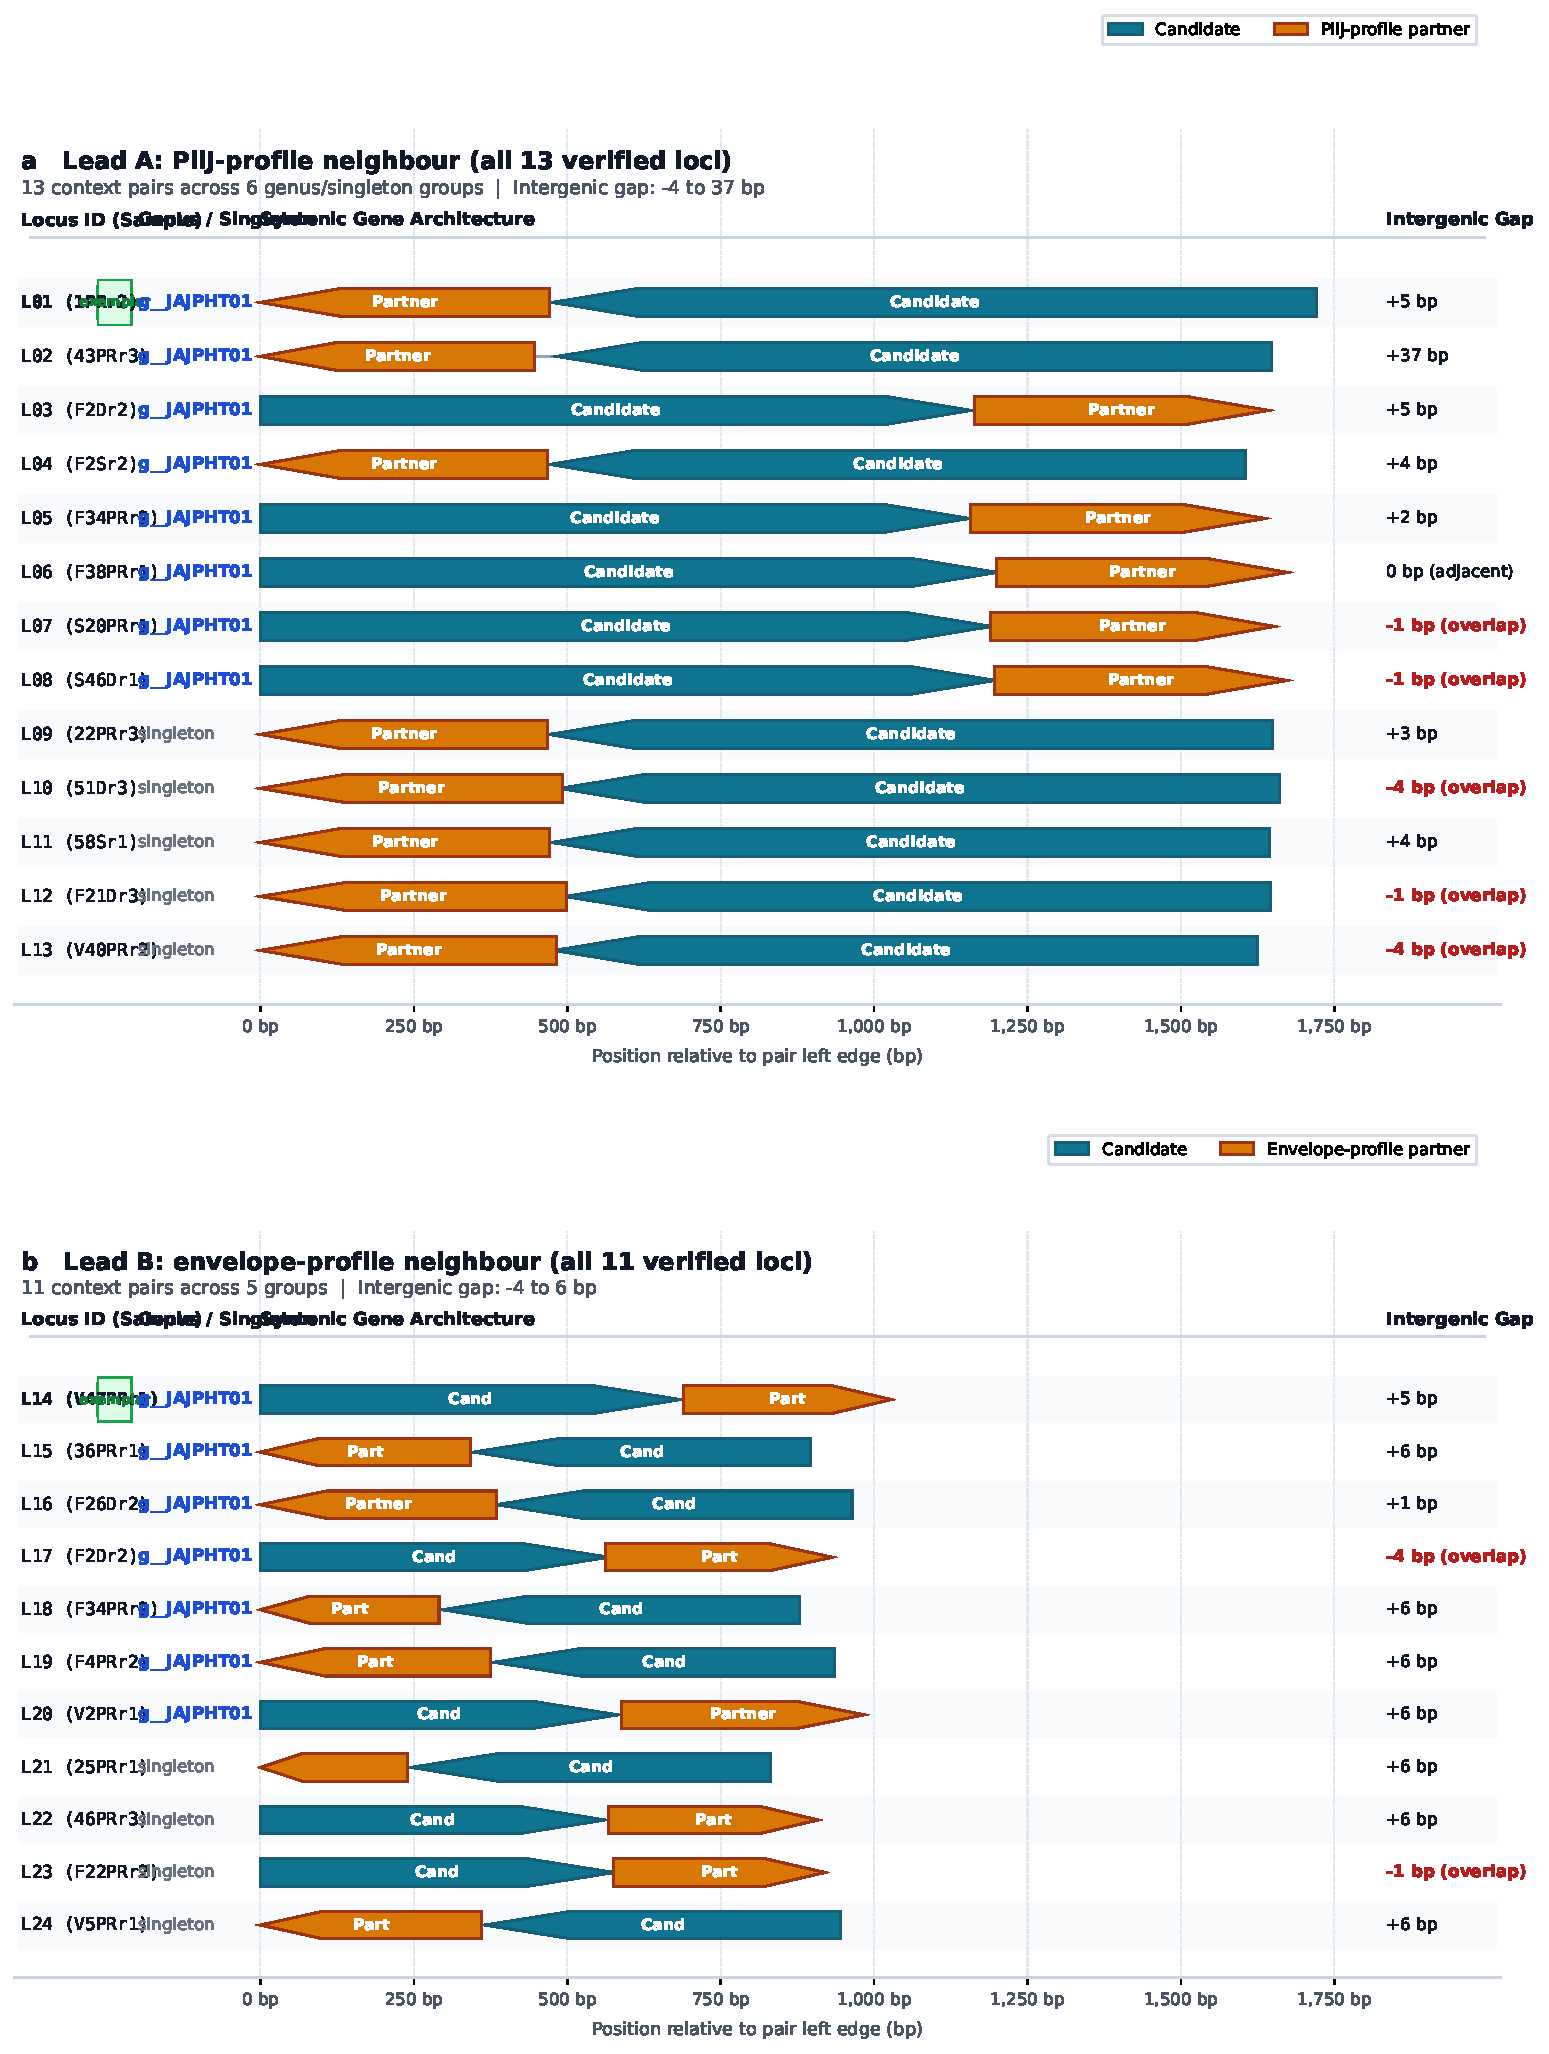
\includegraphics[width=\textwidth,height=0.79\textheight,keepaspectratio]{figures/fig_surface_modules_all_loci.pdf}
\caption{All verified contexts for the two surface-associated leads. Arrows retain native strand orientation and verified nucleotide lengths; coordinates start at the left edge of each pair. Negative intergenic gaps denote overlaps. Locus identifiers resolve to full genome and gene identifiers in the source table. The 24 pairs comprise 13 contexts for lead A and 11 for lead B, all adjacent and co-oriented. Genus-or-singleton labels distinguish named genera from genomes lacking a genus assignment.}
\label{fig:surface_all_loci}
\end{figure}


\section*{Supplementary Methods}

\subsection*{Sampling, sequencing and environmental data}
Soil was sampled on five expeditions along a west to east transect through the Saudi Rub' al-Khali
from the western escarpment ($19.15^\circ$N, $45.17^\circ$E) to the Omani border ($20.71^\circ$N,
$54.73^\circ$E), a cumulative path of 1{,}043~km with 60 numbered sites at predetermined coordinates
and ten named locations. The expeditions ran on 17--20 March 2023, 14 July 2023 (restricted by heat
to eight sites), 17--21 February 2024, 29--31 August 2024 and 12--15 October 2025. At each site and
visit three soil positions were sampled in three co-located replicates: surface soil at 0~cm,
subsurface soil at 5--10~cm, and soil from the root zone at 5--10~cm, termed root-adjacent because
soil was not consistently attached to roots. Soil was held at $-20^\circ$C in the field and at
$-80^\circ$C in the laboratory. Sampling design and field handling are shared with the companion
16S rRNA survey and field-data descriptor \citep{tawfiq2026companion,rubalkhali_datapaper}. The 551 soil samples with complete metadata (117 surface, 166 subsurface, 268 root-adjacent)
are the cohort used throughout; they cover 59 of the 60 numbered transect sites (site 56 has no sequenced sample) and two of the named
locations, recorded under first-expedition labels 62 and 64, giving the 61 sampled locations used in occupancy statistics. Narrower cohorts are defined where used.

DNA was extracted from 0.9--1.2~g of soil with the QIAGEN PowerLyzer PowerSoil kit (12855-50) or the
DNeasy PowerSoil Pro kit (47014), homogenised on a PowerLyzer 24, eluted in 50~$\mu$L and quantified
with the Qubit high-sensitivity double-stranded DNA assay. DNA was fragmented on a Covaris instrument
to 350~bp, purified with AMPure XP beads at 1.6:1, prepared with the QIAseq FX and NEBNext Ultra II
kits and sequenced at KAUST in paired-end mode (150~nt, with 101-nt reads in the fourth-expedition batch) on Illumina NovaSeq 6000 and NovaSeq X instruments.
The submission comprises 554 runs for 551 samples: 221 NovaSeq 6000 runs and 333 NovaSeq X runs
across four sequencing batches. The sample-to-run manifest records instrument, library kit and
batch; three samples have two submitted runs. The exact commands combining those runs remain unverified, and sequencing-batch sensitivity remains unresolved for the exploratory environmental analyses. Reads were
processed with fastp v1.0.1 \citep{chen2018fastp} with base correction in overlapping pairs, a
qualified-base threshold of Q20, at most 40\% unqualified bases per read, a minimum length of 50~nt
and a low-complexity filter at 20\%; surviving pairs and orphaned reads were both retained. The
median sample retained 21.58~Gbp (156.6 million reads; IQR 16.53--25.08~Gbp).

Soil chemistry and climate covariates are those of the companion survey restricted to the samples
profiled here: X-ray fluorescence total elemental contents of archived soil (250 profiled samples
with chemistry; 251 in the family-level cohort) and reanalysis climate series (455 and 456 samples).
Laboratory measurements were made on archived soil with an Olympus Vanta handheld analyser in Fast Mode
(fifth-expedition samples with helium purge and an 8~mm aperture; earlier settings unrecorded) and are distinct
from the fifth-expedition field measurements. Values are instrument-reported magnitudes whose concentration units
are undocumented and consistent with weight percent; detection limits are undocumented, and a recorded zero means
not reported positive \citep{rubalkhali_datapaper}. Climate inputs were
retrieved from the Open-Meteo archive as daily temperature and precipitation series over twelve-month
windows centred on each visit; retained tables record the start and end dates. The provider's model
selection and original API responses were not archived. The de Martonne index divides annualised
precipitation by mean temperature plus ten. The environmental analysis did not include pH.
The complete analysis table rebuilds byte-for-byte from the preserved metadata, laboratory and
climate summary tables; regenerating the original climate retrieval is a separate provenance gap. Three source-table Fe values exceed 45 in the recorded units, and one gives a site-44 median of 22.73; calibration and column metadata are needed to interpret these observations. Family-level sample correlations reuse sites and visits. Site aggregation changes the observational unit and retains between-site variation; interpretation of both analyses depends on spatial structure, compositionality, sequencing batch, extraction kit and measurement metadata.

\subsection*{Assembly, binning, dereplication and taxonomy}
Each sample was assembled with MEGAHIT v1.2.9 \citep{li2015megahit} (\texttt{meta-large} preset,
contigs $\geq 500$~nt, $k$-mers seen at least twice, pruning level 1, low-local-coverage ratio 0.3),
supplying pairs and orphaned reads; 549 of the 551 samples produced an assembly (\texttt{51Sr1}
produced no contigs and \texttt{F5Dr1} an empty file). Assembly statistics used QUAST v5.2.0
\citep{gurevich2013quast}. Every assembly was binned twice with SemiBin2 v2.2.1
\citep{pan2023semibin2}: with the pretrained global model (\texttt{single\_easy\_bin --environment
global --sequencing-type short\_read}) on minimap2 \citep{li2018minimap2} coverage of the paired
reads, and with a self-supervised per-sample model (\texttt{single\_easy\_bin --self-supervised -m
1000}) on BWA-MEM \citep{li2013bwamem} coverage of pairs and orphans. They produced 16{,}333 and
21{,}616 bins of at least medium quality, 37{,}949 in the union of the two unrefined binnings. The
two bin sets were reconciled per sample with DAS\_Tool v1.1.7 \citep{sieber2018dastool} at its
defaults (score threshold 0.5, DIAMOND search); of 542 samples binned by both runs, 539 yielded
refined bins, 14{,}426 in total. Quality was estimated with CheckM2 v1.1.0 \citep{chklovski2023checkm2}
and tiered by completeness and contamination alone: near-complete at completeness $\geq 90\%$ and
contamination $\leq 5\%$ (4{,}225), medium at $\geq 50\%$ and $\leq 10\%$ inclusive (8{,}209; two
bins sit at exactly 10.0\%), the rest below these thresholds (1{,}992). These operational tiers use CheckM2 alone. Subsequent barrnap v0.9 and tRNAscan-SE v2.0.12 \citep{chan2021trnascan} assessment of representatives required non-partial rRNA hits of at least 80, 900 and 1{,}900 nucleotides for 5S, 16S and 23S, respectively. This assessment found all three rRNAs in 157 genomes and at least 18 tRNA amino-acid types in 3{,}629. Full MIMAG classification gave 126 high-quality and 5{,}312 medium-quality representatives \citep{bowers2017mimag}. No chimerism screen was
run on the 14{,}426 bins; GUNC v1.1.1 \citep{orakov2021gunc} against ProGenomes 3 was run on the ten
order-gap candidates only.

The 12{,}434 bins of at least medium quality were dereplicated with dRep v3.6.2 \citep{olm2017drep}
(fastANI \citep{jain2018fastani}, primary and secondary ANI 0.90 and 0.95, completeness $\geq 50\%$,
contamination $\leq 10\%$, other parameters default; one bin was dropped internally), giving 5{,}438
species representatives (2{,}259 near-complete, 3{,}179 additional genomes meeting the medium-completeness thresholds). Representatives were classified with
GTDB-Tk v2.7.2 \citep{chaumeil2022gtdbtk} (\texttt{classify\_wf}, ANI pre-screen on) against GTDB
release 232 \citep{parks2022gtdb}; 1{,}898 classifications changed relative to an earlier run
against release 226, and every reported taxon is from release 232. The first-empty-rank summary
assigns each representative to the first of the seven ranks from domain to species carrying an empty
label; classes are mutually exclusive. The ten order-gap candidates with adequate marker coverage
were placed on de novo trees (GTDB-Tk \texttt{de\_novo\_wf}) and assessed by relative evolutionary
divergence against release-232 rank intervals; the eleventh candidate (46\% of marker positions
aligned) was excluded from adjudication. All ten assessed genomes passed GUNC (clade separation 0.01--0.32 against a 0.45 threshold). Relative evolutionary divergence placed the two multi-genome clades at genus and family depth; the other six genomes formed single-genome lineages. The assessed clades remained within established orders.



\subsection*{Protein catalogue and the sequence-dark call}
Genes were called on assemblies, so that the catalogue covers unbinned sequence;
the 552 assembly files present at that step are a superset of the 549 canonical assemblies, a
catalogue-level basis that enters no per-sample cohort. Prediction used Pyrodigal v3.7.1 \citep{larralde2022pyrodigal,hyatt2010prodigal}
(\texttt{-p meta --no-stop-codon}, partial genes retained): 753{,}305{,}533 proteins, clustered with
MMseqs2 v18.8cc5c \citep{steinegger2017mmseqs2,steinegger2018linclust} (\texttt{linclust
--min-seq-id 0.9 -c 0.8 --cov-mode 0}) into 449{,}265{,}306 representatives, the unit counted in
every dark rate. Every representative was searched against UniRef50 release 2026\_01
\citep{suzek2015uniref} with \texttt{mmseqs search -s 7.5 -e 1e-3 --max-seqs 10}, a pure E-value
criterion with no identity or coverage filter; a cluster is sequence-dark when the searched representative
returned no hit. A cluster is genome-resolved when any member lies on a contig assigned to one of the
37{,}949 unrefined bins of at least medium quality, tested over every member; this membership rule
defines the 43{,}423{,}322 genome-resolved representatives and the 4{,}292{,}446
dark ones among them. Functional annotation of the 5{,}438 representatives used Bakta v1.12.0
\citep{schwengers2021bakta} for gene calling and eggNOG-mapper v2.1.13 \citep{cantalapiedra2021eggnog}
with DIAMOND v2.0.15 \citep{buchfink2021diamond} against the v2.1.12 reference data for KEGG
orthologues. Representatives that refinement emitted as strict contig subsets of a parent bin were
annotated by restricting the parent's gene calls to their own contigs; the resulting orthologue table has no empty rows.

\subsection*{Read recruitment and detection}
Two recruitment runs underlie the paper. The representative-level run mapped each sample's paired
reads to the 5{,}438 representatives with CoverM v0.7.0 \citep{aroney2025coverm} in genome mode
(\texttt{-p minimap2-sr -m relative\_abundance}, all other parameters default). No explicit read-identity or aligned-read-fraction thresholds were set for this genome-level run. The default minimum
covered fraction of 10\% defines detection: a representative is detected when its relative abundance
exceeds zero, that is, when at least a tenth of its genome is covered. The summary, stress and Thermoplasmatota analyses use the 550 usable current profiles (F5Dr1 contained no usable abundance values), which give 45 sites with both surface and subsurface profiled; the main Thermoplasmatota result uses the within-visit pairing specified in the main Methods and Supplementary Note S3. Community values use two denominators: the share of all reads (organisms outside
the catalogue counted as non-carriers, a lower bound) and the share of reads mapping to any
representative (median unmapped fraction near 51\%). The member-aware run mapped the reads of all 551
samples to the 536{,}437 dark-family member genes in contig mode (\texttt{-m tpm covered\_fraction}).
A family is present when any member gene reaches a covered fraction of 0.5 and its abundance is the
summed member TPM. That rule is easier to satisfy for a short gene and reverses the length to
occupancy relation when replaced by any-read presence, so occupancy is compared within length strata.
The two shotgun control libraries sequenced with the fourth expedition, a no-template extraction
control (335{,}190 read pairs after filtering) and a positive control of \emph{Hafnia paralvei}
(119{,}683{,}914 pairs; GTDB-Tk R232 on its assembly, ANI 98.99\%), were profiled with the identical
CoverM invocation and index. Representatives detected in the no-template control are annotated as
reagent contaminants in the catalogue table; the pathogen summary is not reported. The no-template assembly (11 contigs, 11~kb) was identified by UniRef50
search of its predicted proteins. The read-profile signals identify \emph{Escherichia coli} (V42PRr2\_\_single\_SemiBin\_33) and \emph{Cutibacterium acnes} (51Dr3\_\_single\_SemiBin\_390). A separate contig-alignment screen flags ten additional representatives, including the \emph{Mixta alhagi} representative T5PRr1\_\_self\_SemiBin\_614; a vector-matching segment flags a possible contaminant contribution within the matching region. Across these twelve representatives, the lineage-analysis table contains 42{,}831 Pyrodigal protein instances, including 1{,}792 dark instances, out of 20{,}379{,}930 and 1{,}600{,}067, respectively. These instance denominators differ from the genome-linked cluster and Bakta orthologue denominators. Excluding the twelve changes the catalogue median per-genome dark fraction from 6.31\% to 6.34\%; abundance-weighted environmental effects require a separate sensitivity analysis.

\subsection*{Dark families, matched control and selection}
The 4{,}292{,}446 genome-resolved dark representatives were clustered with MMseqs2
\texttt{easy-cluster} (\texttt{--min-seq-id 0.5 -c 0.8 --cov-mode 0}, default sensitivity 4) and each
cluster mapped through the 90\%-identity membership table to the samples and sites in which its
instances were assembled. A cluster was admitted as a dark family when it held at least three
distinct 90\%-identity representatives assembled in at least three samples and two sites (106{,}042
families, 536{,}437 member genes; 2{,}784 three-member clusters failing the spread criterion were dropped). Member nucleotide sequences were excised from the assemblies using the
prediction coordinates. The control pool comprised every non-dark representative on a contig of the
same 37{,}949 bins, with darkness excluded against the assembly-wide dark set. Because dark
representatives are short, the pool was sampled per 10-residue length bin to reproduce the dark
length distribution (seed 20260813; the sample ran 12.5\% short of target, in the 20--39 residue
bins), clustered identically, and control families were drawn to match dark families by size bin
(3--9 exactly, 10--19, 20 or more), one per dark family. Two asymmetries are disclosed: control
families were admitted on member count alone, without the sample and site gate, and after admission
the dark query set is longer than the control (median 105 against 75 residues). These differences, together with the divergent dS distributions, affect comparability; their
direction and size depend on the endpoint. Family admission uses the unrefined bins; phylum attribution traces each member
through its contig to the refined bin, the dereplicated representative and its release-232
classification, which attributes 78{,}727 families.

For each family with at least three usable coding sequences ($\geq 90$~nt, translatable under table
11 without internal stops, protein $\geq 25$ residues), proteins were aligned with MAFFT v7.526
(\texttt{--auto}) \citep{katoh2013mafft} and back-translated to codons. Pairwise dN and dS were computed
by the Nei--Gojobori method \citep{nei1986dnds} (Biopython v1.87 \citep{cock2009biopython}) over at most
80 deterministically thinned pairs per family, retaining pairs with at least 30 codons after removal
of gapped or ambiguous positions, excluding identical pairs and requiring $0 < \mathrm{dS} \leq 2$.
The family statistic is the median pairwise dN/dS (97{,}200 dark and 95{,}647 control families).
For the joint sensitivity comparison, we extracted median coding-sequence length and GC
fraction from all indexed family FASTA sequences of at least 90 nt, before the usable-sequence filters for dN/dS. We formed strata using mean dS boundaries
0, 0.1, 0.25, 0.5, 1 and 2; coding-sequence length boundaries 0, 60, 100, 200 and 400 amino-acid
equivalents; GC bins of width 0.05; and aligned sequence-count boundaries 0, 5, 10 and 20.
The final length and count bins were open-ended. Within each stratum represented in both arms,
we sampled the smaller arm's count from each arm without replacement (seed 20261013).
We repeated selection for seeds 20261013--20261032 and reported covariate balance and median
differences. Seed ranges measure selection sensitivity. Divergence-stratum median differences used 1{,}000 independent family bootstrap replicates per arm (seed 20261014), with 2.5th and 97.5th percentiles. These intervals condition on the observed strata and assume family independence. Strata were left-closed; the final dS bin included 2. Weighted mean contrasts averaged within-stratum mean differences using dark-arm counts, control-arm counts or the smaller arm count. This comparison conditions on the retained common-support families; shared ancestry
and the original family-construction process remain sources of dependence.

The null arm reads the same member genes in the +1 frame: the first nucleotide is dropped, the
sequence trimmed to a codon multiple, every codon translating to a stop under table 11 masked to NNN
(removed by the existing pairwise gap and ambiguity stripping), and all other filters left identical.
It was run on a seeded subset of 10{,}000 families with at least three indexed coding
sequences (seed 20260920), together with the same input subset in the annotated frame. Stop
codons were masked in both calibration arms. An input audit found terminal stops in 43{,}953 of
50{,}898 sequences and internal stops in 21 sequences from 16 families. The null, annotated-frame and paired output sets
contain 9{,}148, 9{,}182 and 9{,}029 families, respectively. A shifted frame inherits the composition and
substitution pattern of the real gene, so this null tests whether the annotated frame is the selected
one. Expedition persistence counts
expeditions with presence under the member-aware rule; re-assembly persistence counts expeditions in
which an instance was independently assembled. Threshold robustness reclustered the same
representatives at 30\% identity.
The exploratory expedition-label null used the 106{,}042-family by 551-sample binary detection matrix. Within each of 159 site-by-soil-position strata, we permuted expedition labels and applied the same global permutation to every family, preserving all family occupancies, co-occurrence patterns and stratum-specific expedition sample counts. Of these strata, 121 contained multiple expedition labels (509 samples). We used 499 permutations (seed 20261015), reporting the all-five frequency, central null quantiles and tail proportions with a plus-one correction. Six fixed occupancy bins were retained as descriptive sensitivities. A sensitivity preserved all samples from each site--position--expedition visit as a bundle and permuted visit labels only among visits of equal replicate count within site and position (499 permutations, seed 20261017). This retained expedition sample counts and within-visit replicate dependence. Of 414 visits, 294 visits containing 342 samples were exchangeable across 238 strata. Label exchangeability within strata is an assumption; sequencing and mapping differences associated with expedition remain possible explanations.

AntiFam v8.0 (278 profiles, release 12 October 2023) was searched with HMMER
\texttt{hmmsearch --cut\_ga} against all genome-resolved dark representatives and the control
protein pool. Matches flagged 3{,}385 dark proteins, including 141 members of admitted families.
A family was flagged when any admitted member matched. For the overlap audit, original Pyrodigal
FASTA-header coordinates were verified for all 536{,}437 admitted members, then intersected with
opposite-strand calls from the same sample and contig. A candidate required overlap covering at
least 50\% of the dark call. The opposing call's darkness was resolved through the complete
90\%-identity cluster membership and assembly-wide dark-ID tables. This audit is conditional on
the gene caller retaining both ORFs. The original Prodigal algorithm limits opposite-strand overlaps to 200 bp between 3' ends and excludes 5'-end overlap \citep{hyatt2010prodigal}; the largest observed co-retained overlap here was 195 nt. The audit therefore has little power for alternatives suppressed by the caller. Sensitivity exclusions used the union of family flags.

\subsection*{Coding-sequence and gene-call validation}
RNAcode inputs used the member coding sequences of each family, trimmed to whole codons; members shorter than 90 nt and duplicate sequences were removed, and families with fewer than three distinct members were not evaluable. Up to 29 members besides the representative were drawn with a family-specific seed. Proteins were translated with the bacterial code, aligned with MAFFT \texttt{--auto} and back-translated to codon alignments with the representative as the reference row. RNAcode used 200 samples for $p$-value estimation and reported all high-scoring segments; the annotated frame was frame 1 on the reference strand. The null copy permuted alignment columns with a family-specific seed.

Gene-call reconciliation compared the protein calls of each species representative with catalogue calls on the same contig. Calls with identical coordinates and strand were identical; other classes recorded shared stop codons, shared starts or overlap with another call, and calls without an overlapping catalogue call on the same strand had no counterpart. Dark status was taken from the matched catalogue call's 90\%-identity cluster, or from an exact sequence match elsewhere in the catalogue.

The spurious-call null shuffled each contig of the 552 assembly files independently with \texttt{esl-shuffle -d}, which preserves mononucleotide and dinucleotide composition and contig length, and called genes with Pyrodigal v3.7.1 in metagenomic mode. Calling the unshuffled contigs with the same settings reproduced the catalogue gene count exactly for the tested assembly. Initiation features (start codon and ribosome-binding motif class) were taken from the Pyrodigal annotation of real and shuffled calls. For the recurrence test, shuffled proteins on contigs assigned to any unrefined bin were clustered at 90\% identity and 80\% coverage with MMseqs2 \texttt{linclust}, and the representatives at 50\% identity and 80\% coverage with \texttt{cluster}. Every shuffled protein was treated as dark. Admission used the dark-family rules: at least three 90\%-identity representatives, members assembled in at least three samples and at least two sites. Shuffled representatives were also searched against the 106,042 admitted dark family representatives with the 50\%-identity and 80\%-coverage criterion.

Read-level pN/pS used a reference of all 536,437 dark and 548,831 control family member genes trimmed to whole codons. Paired fastp-filtered reads of each sample were aligned with Bowtie2 \texttt{--very-sensitive} in end-to-end mode, retaining mapped reads. inStrain \texttt{profile} ran in database mode, with each family treated as one genome for its coverage filter and default read and variant filters (minimum read-pair identity 0.95, minimum coverage 5, minimum variant frequency 0.05).

\subsection*{Cultured-genome comparison}
Long-read genomes recovered from 722 cultured assemblies from saline pans, oases and campground soils of the
same basin (companion pangenome catalogue) were compared with the 5{,}438 representatives by skani
v0.3.1 \citep{shaw2023skani} (\texttt{sketch}, \texttt{search -s 75}); a shared species required ANI $\geq 95\%$ and aligned
fraction $\geq 30\%$. The Bakta proteomes of all 722 cultured genomes (3{,}024{,}784 proteins) were
searched against UniRef50 release 2026\_01 with the identical MMseqs2 rule, so cultured darkness is per protein under
the same call as catalogue darkness, which is per cluster representative. Because several cultured strains map to one representative,
the rate comparison was paired by species: one cultured aggregate against one representative, each
cultured genome assigned to its best-ANI representative, giving 23 pairs from the 25 shared species,
before contaminant exclusion. We excluded representative \texttt{V42PRr2\_\_single\_SemiBin\_33},
identified as \emph{E. coli} in the no-template control, leaving 22 groups for the paired rate
comparison by Wilcoxon signed-rank. Protein sharing used the best-ANI cultured genome of each
representative and reciprocal best DIAMOND hits (\texttt{--very-sensitive -e 1e-5 -k 5}),
requiring at least 50\% identity and 50\% coverage of both proteins. Sharing percentages pool
protein counts across the 22 pairs. The complete-call sensitivity subset contains 166 dark MAG
proteins of at least 100 residues. Gene callers differ (Bakta on cultured genomes, Pyrodigal
on assemblies).

For the nucleotide sensitivity search, we extracted each MAG gene's recorded interval from its
dereplicated representative assembly and retained intervals of at least 90 nucleotides. Each was
aligned to the paired culture-derived assembly using minimap2 v2.17-r943-dirty
(\texttt{-c -x sr -k 11 -w 5 -n 2 -m 20 --secondary=yes -N 20}). Support required a single
alignment spanning at least 90\% of the query with at least 95\% nucleotide identity, calculated
as matching bases divided by alignment block length. Counts were stratified by darkness and
reciprocal protein-hit status. Input assemblies, gene-coordinate tables and protein-search outputs
are identified in the analysis checksum manifest. Recovery of the protein-shared subset provides
a positive comparison for this search's sensitivity. Per-pair recovery and a post hoc restriction to pairs with at least
90\% recovery were reported. All qualifying alignments were checked at identity thresholds
0.85, 0.90 and 0.95. For all DNA-supported calls, culture Bakta CDS coordinates were
intersected with each alignment's target span. A CDS had to cover at least half that span;
orientation and phase at the first aligned position defined a diagnostic category, with
same-orientation phase compatibility taking precedence if several alignments qualified. Eligible dark calls were traced through the complete 90\%-identity cluster table into the admitted-family membership table. Indels
can change phase downstream; this diagnostic evaluates phase at the alignment start.

For exploratory caller substitution, we called the 22 culture assemblies with Pyrodigal v3.7.1 in metagenomic mode (\texttt{-p meta --no-stop-codon}), matching the original MAG-caller configuration while holding nucleotide alignments and eligible MAG calls fixed. The locus-overlap classification was applied to each caller's GFF at 50\% and 90\% of aligned target span; at 50\%, all 68{,}537 Bakta classifications reproduced the retained locus audit. Subsets used the original complete-call flag, exact protein length of at least 100 residues, and admitted-family membership. We retained per-genome-pair transitions and treated calls as descriptive observations. The 90\% criterion gave dark no-CDS counts of 400/735 with Bakta and 281/735 with Pyrodigal; the admitted-family subset remained 18/42 with each caller. The substitution assesses annotation sensitivity at DNA-supported loci; full codon correspondence and translation require additional evidence.

\subsection*{Lineage-associated protein content}
The relationship with reference naming depth is shown in Fig.~\ref{fig:lineage}b. For each representative, every protein on its contigs was traced to its 90\%-identity cluster and
scored dark or not by the cluster call above; the dark fraction is the share of dark protein
instances, computed on the refined winner contigs of all 5{,}438 representatives (native key, no
renaming). Ordinary least squares (statsmodels v0.14.2) modelled the dark fraction on assembly quality
(completeness, contamination, $\log_{10}$~N50, $\log_{10}$~length), then adding phylum and genus
(genera with fewer than five representatives pooled; unnamed genera one level); unique and shared
variance are differences of $R^2$ between nested models. Placeholder-name depth was coded as the first rank with an empty or digit-bearing label, separately from the taxonomy summary of empty ranks and added to the quality model before phylum. No
phylogenetic mixed model was fitted, so the representatives enter as independent draws. Genome size
was completeness-corrected length. The archaeal contrast is a 1:1 nearest-neighbour match without
replacement on standardised completeness, contamination, $\log_{10}$ corrected size,
$\log_{10}$~N50, $\log_{10}$ mean relative abundance and prevalence (samples detected), against two
pools reported separately, other archaea and bacteria, at calipers of 0.5 to 2.0 standardised units
(0.25 also against bacteria); reported pairs use calipers of 1.0 against other archaea and 0.5 against bacteria. Residual imbalance is reported as standardised mean differences. Dark-family attribution by
phylum uses the 78{,}727 attributable families; enrichment is the phylum's share of single-phylum
dark families divided by its share of species, and its share of dark protein instances divided by
its share of all protein instances. The class placement of the Thermoplasmatota representatives was
displayed on an approximate-maximum-likelihood tree (FastTree, LG with gamma; \citep{price2010fasttree}) of the GTDB-Tk
release-232 archaeal marker alignment, with the 1{,}647 release-232 Thermoplasmatota species
representatives and 30 Halobacteriota and Thermoproteota outgroups; the tree supports no branching
claim.

The metabolic comparison used a separate 1:1 greedy nearest-neighbour match without replacement
on CheckM2 completeness, with a caliper of one percentage point: 181 pairs with Halobacteriota,
216 with other archaea (including Halobacteriota), and 237 with bacteria. We report full-lineage
prevalences separately from paired-subset prevalences. KEGG module calls required at least
two thirds of the top-level steps, each satisfied by any listed alternative orthologue.
Custom marker sets required specified subunit counts: cytochrome c oxidase required both
K02274 and K02275; archaellum markers required two of nine orthologues; CRISPR markers required
one of seven; catalase required one of K03781, K03782 or K07217. The carbon-skeleton and sugar
transport sets required two of five and two of six orthologues, respectively. The complete
orthologue lists and module rules are retained with the metabolic-analysis source code.

\subsection*{Within-lineage reference proximity and flanking-gene recurrence}
For each of the 237 Thermoplasmatota representatives, the external comparator was the genome
with the highest mean amino-acid identity among reciprocal best hits, requiring at least 100
reciprocal pairs. The comparator pool contained 218 GTDB R232 and 29 non-duplicate MGnify genomes
in classes SW-10-69-26 and E2. Proteins were predicted independently with Pyrodigal v3.7.1 in
single-genome mode and searched with DIAMOND v2.1.16, using \texttt{--very-sensitive},
$E\leq10^{-5}$, identity $\geq30\%$, and query and subject coverage $\geq70\%$.
The 237 selected pairs used 32 distinct reference genomes. The response was the catalogue dark
fraction, with predictors comprising amino-acid identity, the reciprocal-hit count divided by
the desert genome's single-genome protein count, CheckM2 completeness and contamination, and
base-10 logarithms of assembly length and N50. We fitted phylogenetic generalised least squares
on an approximate maximum-likelihood FastTree phylogeny (LG+Gamma) from the GTDB-Tk R232 ar53 alignment \citep{price2010fasttree}, normalising shared branch lengths to a correlation
matrix and estimating Pagel's $\lambda$ by profile maximum likelihood. Coefficient standard
errors and two-sided tests condition on the fitted covariance and tree. Supplementary Note S2
reports the covariance, denominator, lineage-subset and caller-completeness sensitivities.
None of the 237 representatives had a known relative within the species radius: none reached 95\% average nucleotide identity to the 218 GTDB R232 species representatives of the two classes or to 29 further MGnify genomes. The median amino-acid identity to the nearest known genome was 64.8\%, below the 75.4\% median among congeneric GTDB representatives, and the nearest other desert representative lay at a median 73.1\%.

Species-radius relatives were tested with skani v0.3.1 (ANI $\geq95\%$) against the same comparator pool; the congeneric reference is the median amino-acid identity between GTDB R232 species representatives sharing a genus in the two classes, and amino-acid identity used the same reciprocal-best-hit rule.

For the genomic-context analysis, we compared the 1{,}031 confidence-qualified dark structural
families below the dual-reference query-normalised threshold with the other 1{,}807 qualified
dark families. Family members were mapped to refined-bin contigs and 95\%-ANI species groups;
1{,}461 families occurred in at least two species. We selected one locus per family and species by descending complete-window eligibility, first
for exact-coordinate windows and then for the same-strand stop-match sensitivity. Ties used
descending counts of exact-mapped, exact-or-stop-mapped and present flanks, followed by contig
length and gene count, then ascending member identifier. This ordering uses mapping completeness
and assembly properties independently of flanking orthologue identity. Contig mappings to Bakta
annotations required nucleotide-sequence hashes and the original identifiers in Bakta logs.
The primary window comprised the two predicted genes on each side of the focal gene, with all
four flanks matched to Bakta by exact coordinates and strand. A family was evaluable when such
windows were available in at least two species. Recurrence meant that at least one flanking KEGG
orthologue occurred around that family in two or more species, irrespective of flank position.
We estimated a family-specific background from 5{,}000 draws of eligible pseudo-focal positions
on the same contigs. The primary between-group contrast used excess recurrence above this
background, weighted within common-support strata of species breadth, coarse host phylum and
flanking annotation opportunity. Two-sided label permutations used 10{,}000 draws and a plus-one
correction. Sensitivities included unique same-strand 3$'$-stop matches, exact-phylum and
length-matched pairs, and a species-disjoint family subset (Supplementary Note S2).

\subsection*{Structural analysis}
Queries were the 1{,}466{,}943 genome-resolved dark representatives of at least 100 residues. 3Di
strings were predicted with ProstT5 \citep{heinzinger2024prostt5} through Foldseek
\citep{vankempen2024foldseek} (\texttt{createdb --prostt5-model}) and searched
(\texttt{--alignment-type 2 -s 9.5 -e 1e-3 --max-seqs 50}) against the AlphaFold Database v6 on
UniProt 2025\_03 (241{,}070{,}489 entries) \citep{varadi2024alphafolddb} and the PDB release of 1
January 2025 (324{,}204 chains in the Foldseek database) \citep{berman2000pdb}. Queries with no hit
in either were clustered in structure space (\texttt{cluster --single-step-clustering --cluster-mode
2 -s 4}) and clusters of at least three members admitted as fold families (17{,}221). One model per
family was folded with ESMFold \citep{lin2023esmfold} (\texttt{esmfold\_v1}, transformers v4.40.2,
PyTorch v2.2.2, half-precision trunk, sequences truncated at 1{,}022 residues, four recycles), except
that 3{,}451 families reused a member's existing ESMFold model from an earlier candidate set; those
reused representatives come from a novelty-enriched prior cohort and their dual no-hit rate is higher
(42.8\% against 35.3\% for models folded here), and the dual no-hit count (1{,}031 of 2{,}838) holds when they are excluded.
Models were screened as coordinates (\texttt{--alignment-type 1 -e 10 -s 9.5 --max-seqs 50})
against the same references. 3Di prediction, triage and clustering ran on a GPU build of Foldseek
(commit \texttt{8dc75c74}); the validation screen ran on the packaged build \texttt{10-941cd33},
with candidates and controls in one query set under one command. A model enters at length
$\geq 100$ and mean pLDDT $\geq 0.70$; a dual no-hit is a query-normalised TM-score below 0.5 against
both references \citep{zhang2004tmscore}, and a
model returning no row scores zero. The 3{,}684 blinded controls are 1{,}777 complete PDB chains and
1{,}907 deterministic crops matched to an earlier candidate set on length, composition and
partiality, renamed before folding by the same procedure; 3{,}013 passed the gate. Retrieval failures were counted separately from retrieved alignments with scores below threshold.
The primary comparison retains all qualified models; a secondary comparison conditions on at least
one returned alignment. For each query, the maximum query-normalised score was taken across both references.

For the paired region analysis, we searched all 2{,}838 qualified dark models and 3{,}013
qualified controls as complete chains and as confidence-defined regions against the frozen
PDB Foldseek database downloaded on 30 July 2026. A centred 15-residue moving average of
per-residue pLDDT, shortened at chain ends, identified intervals at or above 0.70.
We bridged gaps of at most five residues when their mean unsmoothed pLDDT was at least 0.55,
then retained intervals of at least 50 residues. Each model contributed a positive crop outcome
when any eligible region reached query-normalised TM-score 0.5. Models without eligible
regions remained in the unconditional denominator. Both search arms used Foldseek
\texttt{10-941cd33}, \texttt{--alignment-type 1 -e 10 -s 9.5 --max-seqs 1000}.
Queries reaching the hit cap while remaining unmatched under any exclusion tier were rerun
with \texttt{--max-seqs 5000}. The primary tier removed each control's source PDB entry;
further tiers removed alignments at or above 30\%, 25\% and 20\% sequence identity.
The GPU sensitivity used the same structures and padded frozen reference on a GPU cluster, with
\texttt{--gpu 1 --prefilter-mode 1 --max-seqs 1000}. This changes the retrieval algorithm to
ungapped prefiltering. Supplementary Note S2 reports cap saturation and CPU--GPU disagreement.

The paired analysis uses query-normalised scores throughout. An audit of the Foldseek build's
alignment-normalised score found that its normalisation length omitted one residue from
inclusive alignment spans. The same length also enters the distance scale and optimisation;
exact correction requires rescoring the coordinates. Raw alignment-normalised values are
preserved as software diagnostics. The whole-chain and crop endpoints and the pooled
1{,}031-model dark group depend exclusively on query-normalised scores, whose normalisation
uses the full query length in this implementation.


The 4{,}880 member proteins of
the candidate families, the 1{,}807 other confident dark representatives and the 3{,}013 gate-passing
controls were searched in one run against Pfam-A 38.2 with HMMER v3.3.2 (\texttt{hmmsearch --cut\_ga});
per protein we recorded the number of domains, the fraction of the sequence covered by Pfam
envelopes and the longest uncovered stretch. Of the 4{,}880 member proteins of the 1{,}031 candidate families, 427 (8.75\%) carried a Pfam domain, in 144 of the 1{,}031 families; among the 3{,}013 control structures 90.7\% did.

\subsection*{Functional profiles and sequence-reference comparisons}
Functional-profile agreement is reported in Suppl. Fig.~\ref{fig:reference_supp}a and Supplementary Note S3. The orthologue ceiling is one minus the pooled ratio of Bakta protein-coding genes carrying a KEGG
orthologue to all Bakta protein-coding genes over the 5{,}438 representatives (19{,}186{,}853 genes);
the CheckM2 gene-call denominator gives 58.3\%. Predicted profiles are PICRUSt2 v2.4.1
\citep{douglas2020picrust2} KEGG-orthologue predictions from the companion V3--V4 amplicon survey
(10{,}543 families, 1{,}270 profiles, byte-identical to that study's input) with weighted
nearest-sequenced-taxon indices. Genome-encoded profiles join the orthologue table to the CoverM
profiles, presence being relative abundance above zero; 448 samples carry both profiles (four
amplicon duplicates summed and renormalised; no amplicon-side depth or NSTI filter was applied, and
29 profiles return fewer than the full family set). Per sample we report presence-recall of
genome-encoded orthologues, Spearman correlation over orthologues both methods report, and the count
of genome-encoded orthologues outside the predictor's emitted set; the last is a reference-vintage
gap.
For the exploratory paired-profile null, both matrices were normalised within sample and ranks were computed over their fixed intersection of 8{,}860 orthologue identifiers, including zero ties. We compared the mean matched-sample Spearman correlation with 4{,}999 permutations of PICRUSt sample labels within expedition and soil position (15 blocks, 448 samples), then within expedition, position and site (66 blocks with at least two samples, 146 samples). Only exchangeable samples contributed to each statistic; singleton strata were excluded. Random permutations could retain fixed points. The random generator used seed 20261016 across the two designs; tail proportions used a plus-one correction. A fixed threshold grid of $0$, $10^{-6}$, $10^{-5}$, $10^{-4}$ and $10^{-3}$ was applied to each normalised profile over the union of identifiers. These post hoc tests describe profile agreement and threshold dependence conditional on recovered genomes and prediction references.

Reference absence searched the 106{,}042 dark and 106{,}042 control family representatives in one
file with DIAMOND v2.0.15 (\texttt{blastp --sensitive --evalue 1e-3 -k 1}) against MGnify90
(717{,}738{,}164 cluster representatives \citep{richardson2023mgnify}), GEM (122{,}978{,}191
proteins, 52{,}515 genomes \citep{nayfach2021gem}), the SPIRE species representatives (269{,}496{,}580
proteins from 107{,}008 genomes, Prodigal v2.6.3 \texttt{-p meta} \citep{schmidt2024spire}), the
gene calls of five desert metagenome studies assembled in SPIRE (147{,}531{,}178 proteins: Atacama
PRJNA484015, 6{,}193{,}359; desert trace-gas autotrophy PRJNA657906, 7{,}200{,}701; JGI arid soils,
30{,}569{,}562; JGI Antarctic cold desert, 49{,}206{,}550; JGI Mojave, 54{,}361{,}006) and SMAG
(129{,}550{,}340 proteins called here with Pyrodigal v3.7.1 \texttt{-p meta} from the 40{,}039 soil genomes of
Zenodo record 8223844 \citep{ma2023smag}); 1.387 billion sequences in total. A
representative with no reported hit is absent under this rule. Searching the desert catalogues
as individual databases returns 2{,}544 further families (2.40\%), so cross-catalogue
ordering is descriptive and the content-versus-depth comparison rests on a rarefaction. The SPIRE expectation uses the original 271{,}000{,}000-sequence anchor; the indexed catalogue contains 269{,}496{,}580 sequences. Both query
sets were searched once against MGnify90 at \texttt{--evalue 1 -k 500 --max-hsps 1}. Under random
retention of subjects with probability $p$ a hit remains reportable at the $10^{-3}$ rule only if
$E \leq 10^{-3}/p$, so the probability of no reportable hit is $(1-p)^{h(p)}$ over the $h(p)$ subjects
meeting that bound, and expected absence is its mean over families at $p$ matched to each catalogue's
size. The \texttt{-k} cap inflates the expectation by at most $(1-p)^{500}$, about 1.3\% at the
smallest catalogue. The depth check searched the absent families against the complete MGnify90
2026\_07 set (1{,}661{,}142{,}385 sequences) with MMseqs2 \texttt{search -s 7.5 -e 1e-3 --max-seqs 10};
it uses a different aligner and release and is analysed separately from the DIAMOND sets. This search matched 5.4\% of the previously unmatched dark families and 35.8\% of the initially unmatched control queries, leaving 25.37\% of dark families unmatched. Occupancy of the
absent families uses the member-aware presence matrix over the 61 sampled locations, within length strata.

For the matched-reference comparison, we sampled 1{,}500 genomes without replacement from the
40{,}039 identifiers in SMAG Supplementary Data 2 \citep{ma2023smag}, using sorted identifiers
and Python's random generator with seed 20261014. We retained this SMAG draw and sampled
2{,}055 genomes from the 52{,}515-genome GEM frame for each seed 20261014--20261016.
This fixed count follows $\lceil4{,}500{,}000\times1.05/2{,}300\rceil$; each GEM draw used a
seeded shuffle of sorted identifiers. Both genome sets were called with Pyrodigal v3.7.1
\citep{larralde2022pyrodigal} in metagenomic mode, omitting terminal stop symbols. After
canonicalisation and exact-sequence deduplication within each arm, we sampled at each integer
protein length the smaller of the two available sequence counts. This matches protein counts,
residue totals and the full integer-length distribution. The primary pair contained 4{,}210{,}592 proteins and 1{,}295{,}970{,}055 residues per reference. DIAMOND v2.0.15 searched all
212{,}084 dark and control queries with \texttt{--sensitive -e 1e-3 -k 1}.
Sensitivity comparisons excluded sequences shared between arms before matching, required
\texttt{--id 30} during search, or used GEM's published Prodigal v2.6.3 calls followed by
rematching. We report paired hit-rate differences and five query-length strata: below 100,
100--149, 150--249, 250--399 and at least 400 residues. The three GEM draws quantify comparator
sampling and quota sensitivity conditional on the fixed SMAG sample. Taxonomic composition,
genome quality and reference diversity remain properties of the compared catalogues.

\subsection*{Environmental structure and stress profiles}
Family abundance (TPM) over the 547 environmentally annotated samples was Hellinger-transformed and
compared by Bray--Curtis dissimilarity, excluding families present in fewer than five samples
(105{,}977 retained). Each block was tested by distance-based PERMANOVA \citep{mcardle2001dbrda}
with 999 permutations of samples: soil position (dummy-coded), space (standardised latitude and
longitude), climate (temperature, precipitation, aridity index; $n = 456$) and geochemistry (eleven
standardised axes: S, Cl, Na, Ca, K, Fe, Mn, V, Si, Ti and a summed salinity proxy; $n = 251$), the
latter two also conditioned on space and on space and position. Every block was tested twice, with
permutations free over samples and restricted within site (59 sites); each environmental block kept
$p \leq 0.002$ under the restricted test, geography is untestable within site by construction, and
the vanadium control stayed null (0.88), under within-site permutations. Sequencing depth ($\log_{10}$ filtered bases per sample, from the read-filtering
reports) explains 1.1\% of composition and leaves the geochemistry share beyond space unchanged
(0.089). Variance partitioning \citep{borcard1992varpart} over position, space and
geochemistry was run on the 251-sample chemistry cohort (499 permutations); a Mantel test
\citep{mantel1967} compared Bray--Curtis with great-circle distance. A single vanadium axis run
through the identical PERMANOVA is the negative control. At family level, abundance was correlated
by Spearman rank with each of thirteen elements, the aridity index and a plant-root contrast over
families present in at least 25 samples of the axis subset, Benjamini--Hochberg corrected within
axis; the five most associated axes were re-tested as partial Spearman controlling ranked latitude
and longitude. The salinity proxy (unweighted Na + Cl + S) retained 41\% of its associations under
conditioning and is not used as a family-level axis.

Stress profiles screened a 28-orthologue DNA-damage panel in eight groups and a 13-orthologue
compatible-solute synthesis panel against the
orthologue table, prevalences being fractions of the 5{,}438 representatives. The solute panel contains K00697, K01087, K16055, K13057, K06044, K01236, K06720, K10674, K03692, K05978, K05947, K18818 and K07026. Trehalose carriage accepts K00697 or K16055 or K13057 or the pair K06044/K01236; ectoine uses K06720, glucosylglycerol K03692, and mannosylglycerate either K05947 or K18818. K10674 is reported separately as a hydroxyectoine-associated marker. Strict-route sensitivities require K16055 or both K00697/K01087 for trehalose, both K03692/K05978 for glucosylglycerol, and K18818 or both K05947/K07026 for mannosylglycerate. Community values per
sample used occurrence, whole-community and mapped-community metrics over the 550-sample cohort;
the unmapped fraction does not differ between surface and subsurface (54.4\% against 53.7\%,
Mann--Whitney $p = 0.47$), and root-adjacent comparisons use the mapped denominator. Surface against
subsurface was tested on site medians by Wilcoxon signed-rank over the 45 sites with both positions
profiled, Holm-corrected within metric; effects were re-tested within each of the eight most
abundant phyla (a phylum tested at $\geq 15$ paired sites with $\geq 15$ detected species per
sample) and interpreted only if the direction replicated, which the mismatch-repair contrast failed.
Within-species differentiation compared surface and subsurface member genomes of the 327 species
recovered from both positions (324 with annotations) by Wilcoxon signed-rank. Gradient tests were
partial Spearman on ranked latitude and longitude, with residual degrees of freedom equal to sample count minus four for two independent spatial covariates, against five salt axes ($n = 250$) and three
climate axes ($n = 455$), Benjamini--Hochberg corrected within block; the Halobacteriota association
was re-tested on centred log-ratio fractions and on detection.

Differential encoded function by soil position used the carriage of each feature, the share of the
mapped community whose representatives encode it, over the 549 samples profiled when this analysis was run (before the 51Sr1 profile repair): 282 KEGG modules in
DRAM's step form (present when at least two thirds of steps are encoded; 117 modules absent everywhere
or universal were excluded) and the 4{,}127 orthologues at 5 to 95\% prevalence. Replicates were
collapsed to the median per site, position and visit; root-adjacent minus bulk (the median of surface
and subsurface at the same visit) was taken at 52 sites and surface minus subsurface at 37, each
difference then medianed over visits per site. A feature passed at Benjamini--Hochberg $q < 0.05$
within basis and contrast, an absolute effect of at least 5 percentage points, and the same sign when
carriage was recomputed within Actinomycetota alone and within Pseudomonadota alone (samples where
the phylum held under 1\% of mapped abundance blanked); within-phylum magnitudes are reported beside
each effect. One-step modules are single orthologues or any-of sets and are named by enzyme. Size
normalisation (per Mb of completeness-corrected genome) and restriction to representatives at least
90\% complete were run as sensitivity analyses. Chemistry and expedition contrasts were computed but
are not reported, the former because X-ray fluorescence coverage differs by expedition and the latter
because only eight site pairs qualify.

% P3 LIFE ON AIR: heading was "Trace-gas, biosynthetic and resistance profiles".
\subsection*{Biosynthetic and resistance profiles}
% P3 LIFE ON AIR: moved to the separate life-on-air paper (repository folder lifeonair/), 10 Oct 2026.
% Hydrogenase large subunits (K06281) and carbon-monoxide dehydrogenase large subunits (K03520) were
% retrieved from the Bakta proteomes and classified by DIAMOND best hit against HydDB
% \citep{sondergaard2016hyddb}, high-affinity uptake being groups 1h and 1l
% \citep{greening2016genomic}, and against three form-I CoxL references, form I being called at
% $>55\%$ identity with $\geq 90\%$ coverage or on the AYRGAGR motif \citep{cordero2019atmospheric}. No
% identity or coverage floor was applied to the HydDB call, and 2{,}815 of 4{,}727 CoxL proteins remain
% unresolved, so the form-I count is a floor. Trees were built for display only (MMseqs2, MAFFT,
% FastTree). Five representatives emitted by refinement were removed from the guild after typing.
Biosynthetic gene clusters were detected with antiSMASH v8.0.4 \citep{blin2025antismash8} in minimal
mode on the 5{,}438 genomes, counting per-species presence of a product type; 85.3\% of 44{,}002
regions abut a contig edge, so completeness and novelty are not estimated. Resistance and stress
determinants used AMRFinderPlus v4.2.7 (database 2026-05-15.1, plus set, no organism option, so no
point mutations) \citep{feldgarden2021amrfinderplus}. Because the no-template control assembled into a
laboratory plasmid carrying aph(3')-Ia, a TEM $\beta$-lactamase and a chloramphenicol
acetyltransferase, resistance hits were checked against contigs matching that plasmid: two
aph(3')-Ia hits sit on such contigs, and aph(3')-Ia occurs in seven species in all, five of them on
an identical 7{,}838-bp contig at 100\% identity. Removing every aph(3')-Ia hit lowers aminoglycoside
prevalence from 11.9\% to 11.8\%; no other reported class moves. Ectoine synthesis calls from the orthologue
panel and from antiSMASH were compared as two independent methods (Jaccard 0.921 between the two call sets). None of these profiles has a
matched genome set or size normalisation and they are reported as description; the pathogen summary
of the representatives is not reported because two of its hits are reagent contaminants.

\subsection*{Family-specific sequence, structure and read support}
The targeted family screen used 20{,}451{,}986 Prodigal translations from the 5{,}438 representatives. This caller-specific search space differs from the Bakta CDS set used for the catalogue annotation denominator. External comparisons used the sampled SMAG and GEM protein pools before the length-quota matching described above. Complete predictions required Prodigal \texttt{partial=00} in the original headers or coordinate mappings.

Heliorhodopsin candidates required a PF18761 or NF038020 domain with independent $E\leq10^{-5}$ and profile coverage $\geq70\%$, a higher domain score than the type-1 rhodopsin profile PF01036, and a margin of at least 20 bits over the strongest PF00001/PF00002 control hit, treating absent control hits as zero. HMM alignment to PF18761 located the lysine corresponding to K241 of 48C12 (AVZ43932.1); this residue criterion was applied to all comparison sources. The expanded reference comprised the retained sequences in the published heliorhodopsin alignment of \citet{bulzu2021heliorhodopsin}, figshare version 3 (\url{https://doi.org/10.6084/m9.figshare.13286486.v3}), passing the PF18761 coverage, significance and lysine criteria, together with the curated reference panel. Published alignment-derived sequences can lack terminal residues, and their gene completeness was unavailable. DIAMOND ultra-sensitive searches used $E\leq10^{-3}$ and at least 70\% span coverage of both query and target; identity was reported for the highest-bit-score qualifying hit.

Published SMAG/GEM taxonomy and Rub' al-Khali release-232 assignments were joined to sequence identifiers. Explicit phylum-name aliases reconciled nomenclature; taxonomies were not reclassified against a common release. Exact sequences were deduplicated within source before within-class comparisons. MMseqs2 jointly clustered all sources at 50\% or 80\% identity with 80\% bidirectional coverage. Full-length and profile-core partitions used the same records; cores extended from the first to the last occupied HMM match position, retaining internal insertions. Equal-sized draws used 1{,}000 seeds, $20261015+j$ for $j=0,\ldots,999$. We counted clusters without any member of the expanded reference. A reference-free sensitivity re-clustered only the environmental Saccharimonadia sequences and counted all sampled clusters without reference subtraction. The percentile ranges describe conditional subsampling of these fixed panels. Analytical hypergeometric expectations independently checked the Monte Carlo means.

ProstT5 \citep{heinzinger2024prostt5} encoded all 1{,}744 source records using the AA2fold prefix and residue-only mean pooling. Identical cleaned sequences were encoded once and restored to their original identifiers. Native cosine distances were retained separately from visualisation. For t-SNE, exact sequences were deduplicated across sources, vectors were L2-normalised and reduced to 50 principal components. The displayed projection used perplexity 30, PCA initialisation, seed 42 and 2{,}000 iterations; sensitivities used perplexities 5 and 50 and random initialisations with seeds 123 and 20261015. Projection distances were not used to classify sequence novelty.

ESMFold \citep{lin2023esmfold} predicted each distinct sequence with four recycles and chunk size 64, using checkpoint \texttt{75a3841ee059df2bf4d56688166c8fb459ddd97a}. Per-residue C$\alpha$ pLDDT was converted from the implementation's unit interval to a 0--100 scale. TM-align \citep{zhang2005tmalign} compared full predictions with chain X of the experimental heliorhodopsin structure 6SU3 \citep{kovalev2020heliorhodopsin}; TM-scores were normalised by query length. Predicted structures and confidence values provide sequence-derived structural evidence. Candidate translations were independently reconstructed from the original contigs, allowing the caller's initiation methionine.

Original source-assembly BAMs provided locus read support. SAMtools depth used mapping and base qualities $\geq20$, excluded unmapped, secondary, supplementary, duplicate and QC-failed alignments, and suppressed overlapping mate counts. A locus passed when median depth was at least five and at least 95\% of its bases had depth at least one. For proposed EctCD fusions, distinct read-template names were counted when a single contiguous aligned block spanned at least 20 reference bases on each side of the midpoint between the predicted domains. This junction test used the mapping-quality and flag filters. Retained regional BAMs reproduced the whole-BAM depth output exactly. These checks establish support in the original mappings, conditional on their assembly and mapping specificity.

\subsection*{CPF and EctABC follow-up analyses}
The cryptochrome/photolyase-family (CPF) screen accepted complete genes matching PF00875, PF03441 or PF04244 at independent domain $E\leq10^{-5}$ and profile coverage $\geq70\%$. This operational panel can exclude short photolyases \citep{xu2021shortphotolyases}. EctC candidates required PF06339 or NF009806 at $E\leq10^{-10}$, profile coverage $\geq70\%$ and a 25-bit margin over generic cupin controls PF00190, PF07883 and PF02678. Reference-aligned W21, E57, Y84 and H92 of A0A385TEI2 defined the residue-conserving subset, informed by EctC structural work \citep{czech2019ectc}. EctA/B neighbours required TIGR02406/TIGR02407 at $E\leq10^{-5}$, profile coverage $\geq50\%$, complete genes on the same strand and an edge-to-edge distance of at most 5 kb from EctC. A and B could occupy the same complete ORF when both profiles passed; their domain intervals were inspected separately and reported as putative fusions. A sensitivity raised A/B coverage to 70\%. Actual contig lengths defined edge proximity. Non-ABC loci were conservatively censored when EctC was within 5 kb of an edge or a partial A/B/D marker occurred within that window. EctD used TIGR02408 at the same significance and 50\% coverage thresholds.

Carrier abundance was the fraction of reads assigned to the representative catalogue, after within-sample normalisation. The zero-mapped sample F5Dr1 had no defined catalogue fraction and was excluded. Surface/deep contrasts paired samples within site and expedition, took replicate medians within position and then median visit differences within site. Two-sided Wilcoxon signed-rank tests across sites received Holm correction over six displayed contrasts: CPF, K01669, complete EctABC neighbourhoods, residue-conserving EctC, CPF without K01669 and the stricter A/B-coverage sensitivity. These follow-ups were exploratory and reused the original metagenomes.

A separate arithmetic-mean estimand allowed an exact decomposition. For lineage $g$ present in both positions, let $w_{gp}$ be relative abundance and $f_{gp}$ its carrier fraction in position $p$. With $S$ denoting surface and $D$ deep soil, the between-lineage term was $B=\sum_g(w_{gS}-w_{gD})(f_{gS}+f_{gD})/2$ and the within-lineage term was $W=\sum_g(w_{gS}+w_{gD})(f_{gS}-f_{gD})/2$. The signed carrier abundance of lineages observed in only one position formed $R$, giving the exact total $B+W+R$. Replicate abundances were averaged before decomposition; visit components were then averaged within site and sites weighted equally. We evaluated phylum and genus groupings, assigning each genus-unclassified MAG its own group. Genus-unclassified MAGs accounted for 25.7\% of mean community abundance and were represented as separate groups, whose within-group term is zero by construction. Within-genus changes therefore represent species composition under fixed representative traits. Descriptive percentile intervals used 2{,}000 site bootstrap resamples with seed 20261015; these intervals and the median-based signed-rank tests concern different estimands.

\subsection*{Comparative-analysis diagnostics}
The evolutionary comparison used 106{,}042 UniRef50-matched families, of which 95{,}647 were evaluable, with median dN/dS 0.388 (Fig.~\ref{fig:dark}a,c). In the 10{,}000-family calibration input, annotated- and shifted-frame medians were 0.427 (9{,}182 families) and 1.086 (9{,}029 paired families). The shifted frame gave the higher estimate in 92.4\% of the 9{,}029 families evaluable in both frames (Fig.~\ref{fig:dark}b). Median family mean dS was 0.607 in the dark arm and 0.863 in the annotated arm. At mean dS below 0.1, dark and annotated median dN/dS values were 0.582 and 0.321; at dS 0.5--1.0 they were 0.435 and 0.452. Coarsened matching retained 61{,}427 families per arm, with medians 0.386 and 0.423. In the 553 common strata before equal-count sampling, weighted mean differences were $+0.012$ with dark-arm weights, $-0.022$ with annotated-arm weights and $-0.018$ with overlap weights. These means and the pooled medians are different estimands. Residual dS imbalance after matching was $-0.124$ standardised units. The interpretation of the evolutionary contrast conditions on divergence, family ascertainment and the weighting population. Among 91 evaluable families flagged by AntiFam or opposite-strand overlap, median dN/dS was 0.762 and 76.9\% were below one. Excluding all 102 flagged families left a median of 0.4251 across 97{,}109 evaluable families.

Recruitment frequencies depend on coding-sequence length: all-five-expedition detection was 89.7\% below 60 residues and 67.1\% at 250 residues or more. The expedition-label permutation gave mean all-five frequency 82.7\% (central 95\% range 81.1--84.2\%, lower-tail $p=0.002$); preserving whole visits gave 80.5\% (78.9--82.1\%, $p=0.11$). These tests calibrate the observed 79.4\% against occupancy and the specified exchangeability unit.

Reciprocal protein matches recovered 238 of 1{,}507 dark calls and 65{,}478 of 81{,}723 UniRef50-matched calls. Cultured genomes had a lower dark fraction in 18 of 22 groups (median difference $-0.36$ percentage points, Wilcoxon $p=0.0066$), and 26 of 166 complete dark calls of at least 100 residues had a reciprocal protein partner. For protein-shared calls in the culture comparison, nucleotide alignments recovered 219 of 236 dark calls and 62{,}925 of 65{,}477 UniRef50-matched calls. The union of protein and nucleotide support contained 752/1{,}341 eligible dark calls and 70{,}354/81{,}533 UniRef50-matched calls. Of the 516 DNA-supported dark calls without protein partners, 343 lacked a Bakta CDS covering half the aligned span, 81 overlapped a different frame or orientation, and 92 had compatible orientation and first-base phase. Only 65 eligible dark calls mapped to 47 admitted recurrent families; 42 had nucleotide support, and both callers left 18 of these without CDS overlap. Among all 735 DNA-supported dark calls, 344 lacked a Bakta CDS covering half the aligned span; caller substitution reduced this count to 235. Caller substitution primarily altered the broader call set.

The quality-only regression accounted for 11.5\% of per-genome dark-fraction variance; adding phylum or genus gave 76.8\% or 83.5\%. These descriptive regressions treat genomes as independent and have different degrees of freedom. Quality- and abundance-matched Thermoplasmatota comparisons gave median dark fractions of 0.308 versus 0.048 across 218 archaeal pairs, and 0.310 versus 0.069 across 237 bacterial pairs (Fig.~\ref{fig:lineage}c). Restricting the placeholder-label comparison to class rank gave 0.310 for 236 Thermoplasmatota and 0.125 for 324 other representatives. Phylogenetic dependence and reference naming coverage enter the interpretation of these between-lineage comparisons.

In 181 completeness-matched Thermoplasmatota--Halobacteriota pairs, glyoxylate-module calls occurred in 139 versus 63 genomes, amino-acid carbon-skeleton markers in three versus 165, catalase markers in 49 versus 153, and sugar transport markers in four versus 132. The full Thermoplasmatota set had no detected methanogenesis, ammonia-oxidation or rhodopsin markers. Annotation-based pathway and absence assessments depend on lineage-sensitive model coverage and the specified module rules.

Cropping jointly changes sequence extent, score normalisation and search opportunity. The initial structural screen used 3{,}013 confidence-qualified controls, of which 101 fell below the query threshold. Twenty-two dark models and 66 controls returned no reference alignment. After excluding the source PDB entry, 2{,}889 controls had a matched crop in the paired PDB search. The genomic-context comparison retained 24.16\% of multispecies families under its complete-flank requirement. Methods and Supplementary Note S2 define these selection and retrieval criteria.

The heliorhodopsin analysis was conducted separately from the sequence-dark classification. Two of ten distinct GEM Saccharimonadia sequences occurred exactly in the published reference panel; across all GEM heliorhodopsins, eight of 73 source records had exact published matches. The two SMAG Saccharimonadia sequences were insufficient for the ten-sequence comparison. Reference-relative cluster counts measure addition to the named panel. The environmental-only clustering supplies a separate comparison without reference subtraction, and both analyses condition on the sampled genome collections. Sequence-derived embeddings and structure predictions share their input evidence; t-SNE provides visualisation and sequence clustering supplies the quantitative diversity comparison.

\subsection*{Statistical procedures}
Statistical tests and uncertainty estimates are specified with each analysis. Genome-quality models used ordinary least squares; within-lineage models used phylogenetic generalised least squares. Paired site contrasts used Wilcoxon tests, family-context comparisons used permutations, and matched sequence-search outcomes used paired binary comparisons. Exploratory group comparisons used Mann--Whitney or Kruskal--Wallis tests, with Spearman or partial Spearman correlations for ranked associations. Holm and Benjamini--Hochberg corrections apply within the stated analysis blocks \citep{holm1979multiple,benjamini1995fdr}. Wilson intervals describe binomial proportions where specified. The retained scripts provide software versions, seeds and the observational unit for each analysis.


\clearpage
\renewcommand{\thefigure}{S\arabic{figure}}
\renewcommand{\theHfigure}{S\arabic{figure}}
\setcounter{figure}{0}
\begin{figure}[p]\centering
\includegraphics[width=0.90\textwidth]{figures/fig_dark_current.pdf}
\caption{\textbf{Sequence conservation in recurrent families and sharing with cultured bacteria.}
\textbf{a}, Empirical cumulative distributions of family median dN/dS for 97{,}200 dark and
95{,}647 UniRef50-matched families. The display extends to dN/dS = 2; cumulative fractions use all families.
\textbf{b}, Annotated- and shifted-frame calibration distributions from a 10{,}000-family input,
with 9{,}182 and 9{,}148 evaluable outputs; the display extends to dN/dS = 3.
\textbf{c}, Difference between dark and control family medians in left-closed divergence strata (final bin includes 2), with 95\% intervals from 1,000 family bootstrap replicates. Labels give dark/control counts. Intervals use independent family resampling.
\textbf{d}, Percentage of annotated and dark MAG protein calls with reciprocal protein hits
in the paired culture-derived assembly, for 22 species groups after exclusion of a confirmed
\emph{E. coli} contaminant. Each line joins the two fractions for one MAG. \textbf{e}, DNA support by protein-hit status, with counts above bars. Eligible coding intervals are at least 90 nt; support requires a base-level alignment at 95\% identity and 90\% query coverage. \textbf{f}, Recovery of protein-shared calls by genome pair; the dotted line marks a post hoc 90\% diagnostic threshold.}
\label{fig:dark}
\end{figure}

\begin{figure}[p]\centering
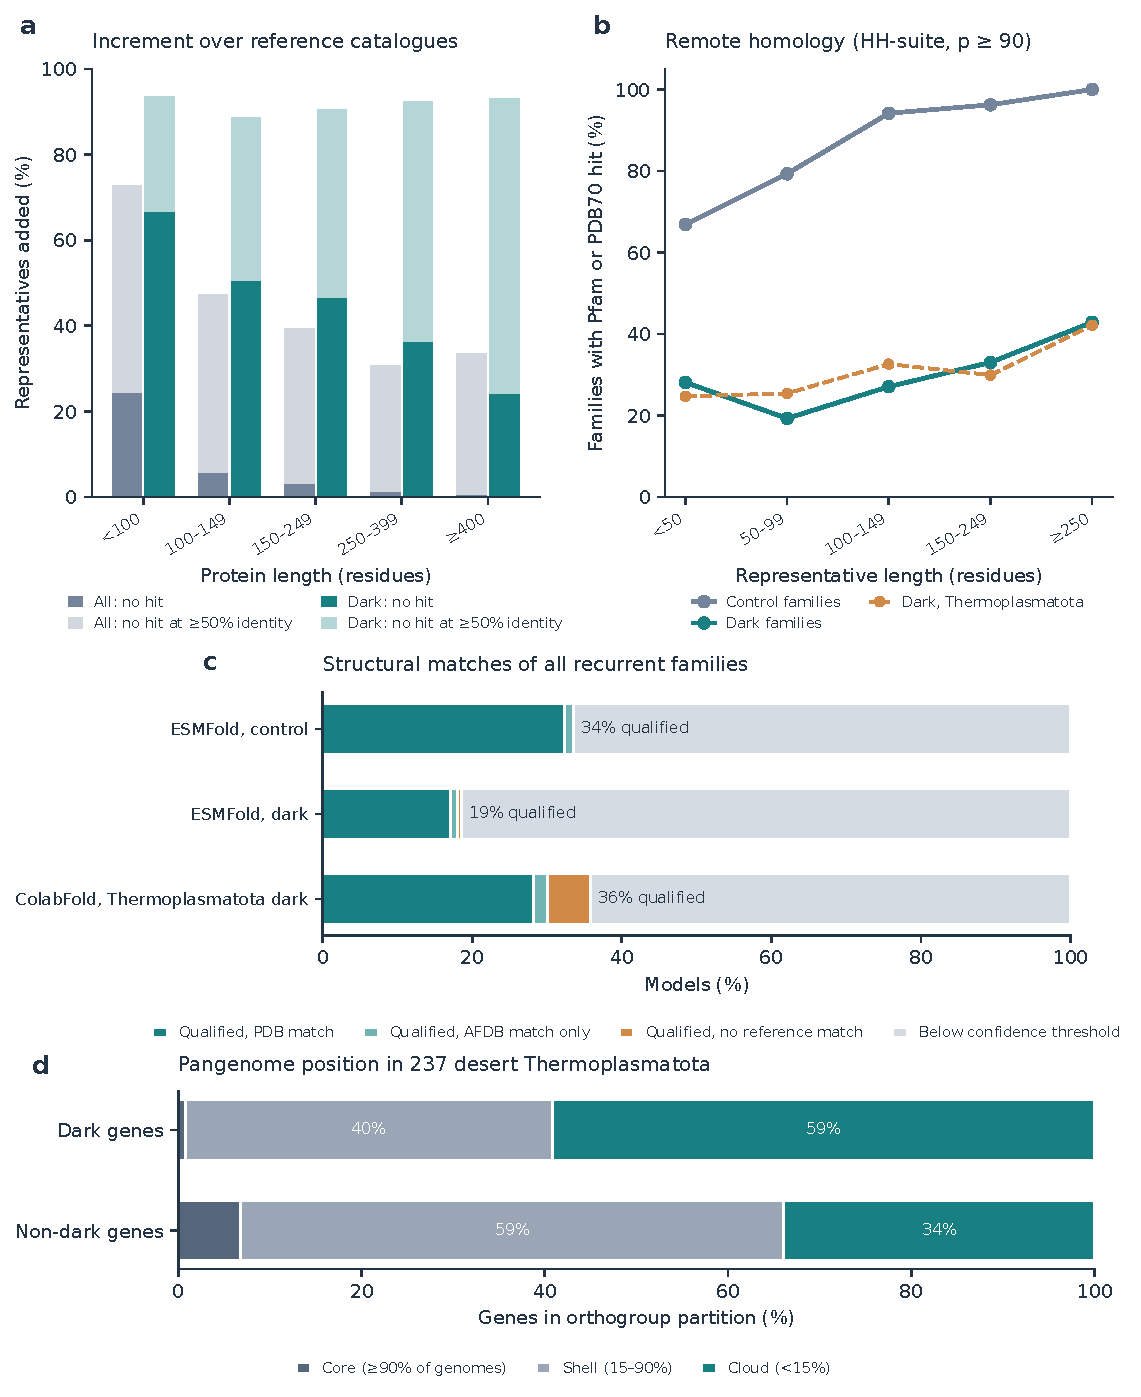
\includegraphics[width=0.92\textwidth]{figures/fig_validation_supp.pdf}
\caption{\textbf{Catalogue increment, remote homology, structural matches and pangenome position of the dark repertoire.}
\textbf{a}, Genome-linked representatives without a hit (solid) or without a hit reaching 50\% identity over 80\% of both sequences (light) in the combined MGnify90, GEM and desert panels, by protein length, for all \unreg{43,423,322} and \unreg{4,292,446} dark representatives.
\textbf{b}, Recurrent families with an HH-suite match to Pfam-A or PDB70 at probability of at least 90\%, by representative length, for dark families, Thermoplasmatota-attributed dark families and a 1,061-family control sample.
\textbf{c}, Structural outcomes of ESMFold models of all recurrent dark and control family representatives, and of ColabFold models of Thermoplasmatota dark families whose ESMFold models were unconfident or absent. Qualified models have at least 100 residues and mean pLDDT of at least 0.70; a PDB match has query-normalised TM-score of at least 0.5 for the whole chain or a confident region.
\textbf{d}, Distribution of dark and other genes of the 237 desert Thermoplasmatota representatives across core, shell and cloud orthogroups.}
\label{fig:validation_supp}
\end{figure}

\begin{figure}[p]\centering
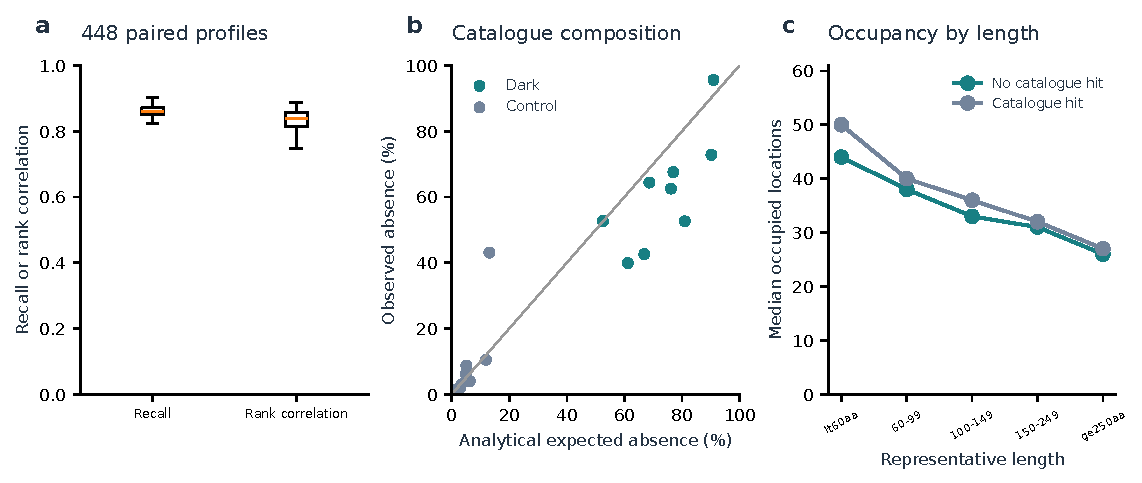
\includegraphics[width=\textwidth]{figures/fig_reference_current.pdf}
\caption{\textbf{Soil references recover widely distributed dark families.} \textbf{a}, Presence-recall of genome-encoded orthologues and rank correlation on shared orthologues across 448 paired profiles. PICRUSt2 emits its full orthologue set in 419 samples at the greater-than-zero threshold; recall therefore largely reflects reference overlap. Boxes show medians and interquartile ranges, with 1.5-interquartile-range whiskers and outliers omitted. \textbf{b}, Observed absence versus the analytical E-value-corrected MGnify90 rarefaction expectation at the indexed catalogue sizes, except the retained SPIRE expectation uses a 271.0-million-sequence anchor for its 269.5-million-sequence index. The diagonal indicates agreement with the size-only expectation. Each point is a catalogue, coloured by query group; points below the diagonal have lower observed absence. Atacama has 4.67 percentage points more dark-family absence and 29.97 points more control-family absence than the size-only expectation, demonstrating a large reference-composition residual. The combined desert and SPIRE annotated residuals are +0.93 and +1.23 points in expected-minus-observed absence. \textbf{c}, Median occupied locations out of 61, stratified by representative length and absence from every searched catalogue. }
\label{fig:reference_supp}
\end{figure}


\begin{figure}[p]\centering
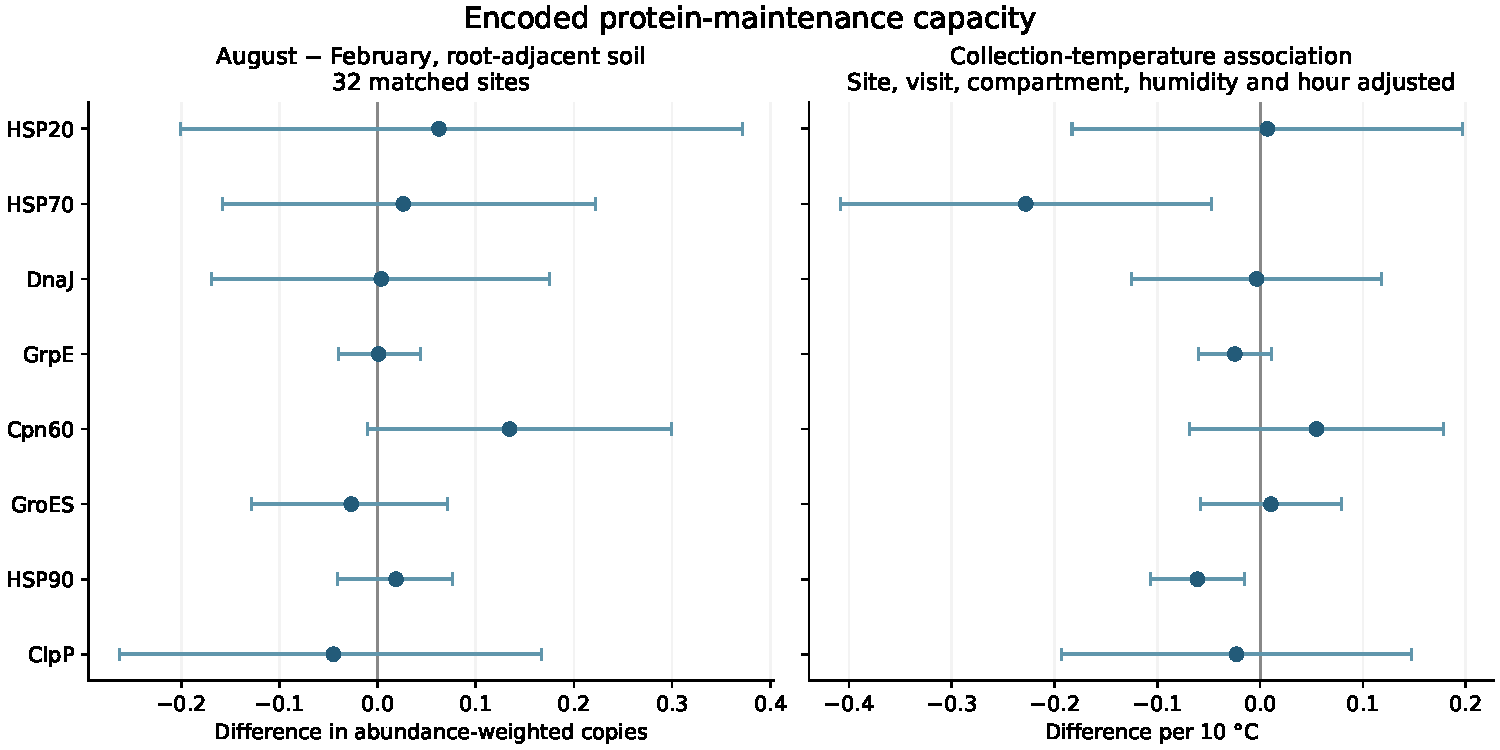
\includegraphics[width=\textwidth]{figures/fig_heat_stress_supp.pdf}
\caption{\textbf{Protein-maintenance capacity across visits and collection temperatures.} Left, August--February differences in community-weighted genomic copies across 32 paired root-adjacent sites, with 95\% intervals from 5{,}000 site bootstrap resamples. Right, temperature coefficients per 10$^{\circ}$C from models including site, visit, compartment, collection hour and humidity, using 391 complete cells from 59 sites; intervals are site-clustered 95\% confidence intervals. Intervals are pointwise; multiplicity-adjusted tests for the displayed comparisons all had $q>0.05$.}
\label{fig:heat}
\end{figure}

\begin{figure}[p]\centering
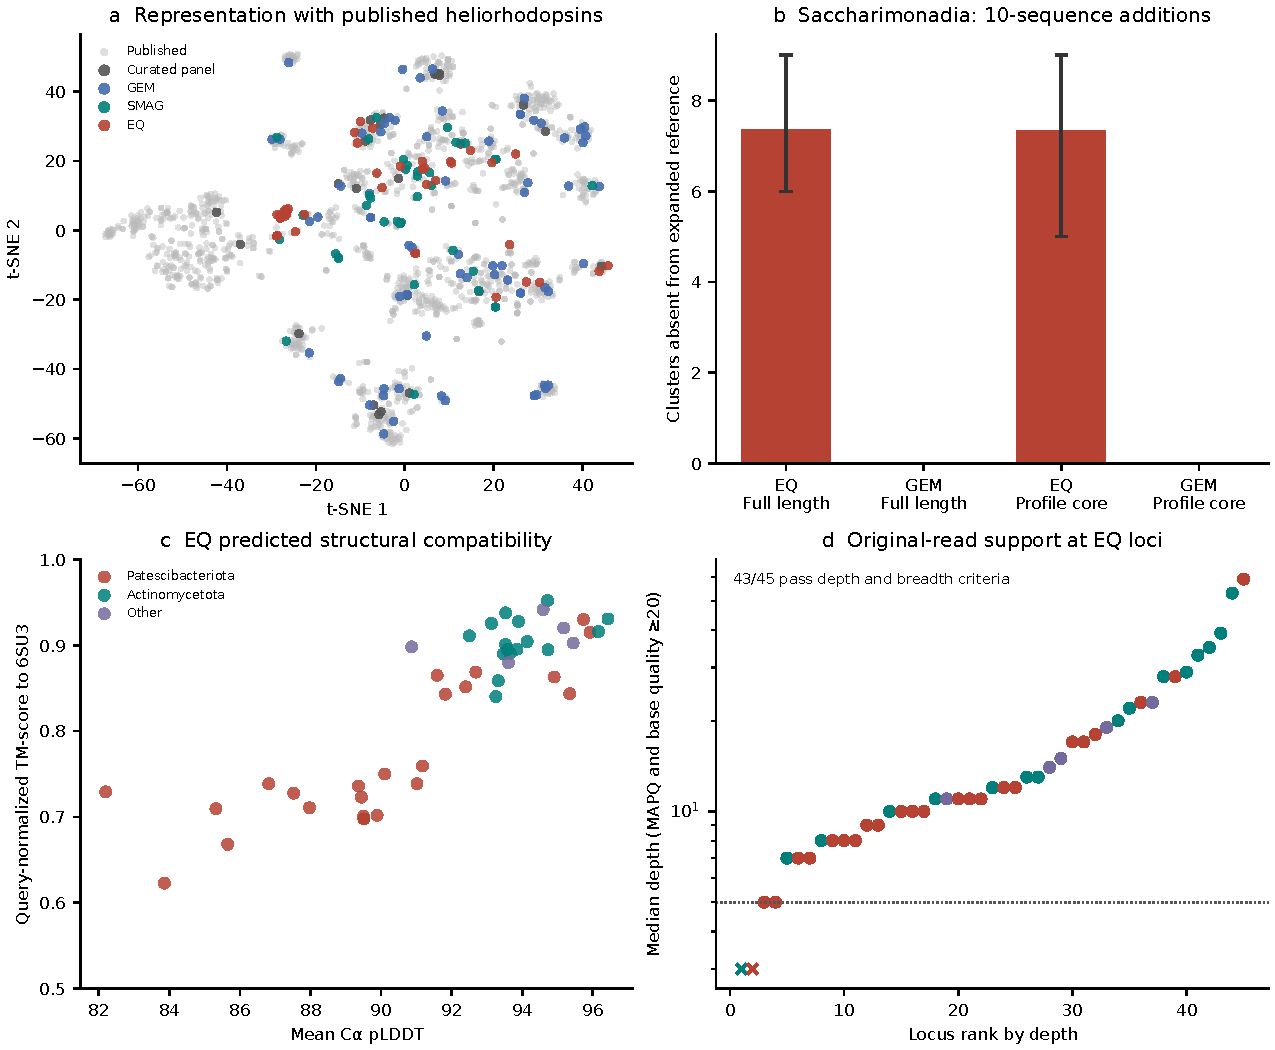
\includegraphics[width=\textwidth]{figures/fig_helio_expanded.pdf}
\caption{\textbf{Desert heliorhodopsins extend sequence diversity around a known fold.} \textbf{a}, ProstT5 t-SNE projection of 1{,}726 unique sequences from the Rub' al-Khali, sampled SMAG/GEM, curated and expanded published panels. The projection displays relationships among the encoded sequences. \textbf{b}, Mean numbers of 50\%-identity clusters absent from the expanded reference after adding ten Saccharimonadia sequences; error bars show the 2.5th--97.5th percentiles of 1{,}000 draws from the fixed source panels. Full-length and profile-core partitions use identical input records. GEM overlaps the published panel, including eight of its 73 source records exactly; zero added clusters indicates coverage by this reference panel. \textbf{c}, Mean C$\alpha$ pLDDT and full-query-normalised TM-score to 6SU3 for 45 Rub' al-Khali models. Terminal extensions contribute to the query-length denominator. These predictions are sequence-derived evidence of fold compatibility. \textbf{d}, Median quality-filtered depth at the 45 Rub' al-Khali loci in original assembly mappings. Crosses mark the two loci failing the depth/breadth rule; the dotted line is depth five. Colours in c and d indicate host phylum.}
\label{fig:helio}
\end{figure}

\begin{figure}[p]\centering
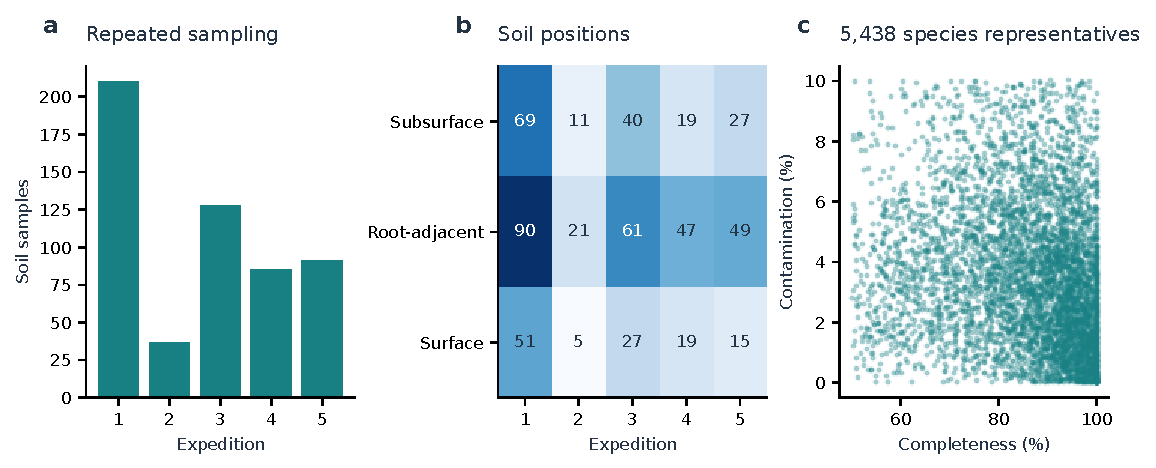
\includegraphics[width=\textwidth]{figures/fig_study_current.pdf}
\caption{\textbf{Sampling and genome quality across the Rub' al-Khali transect.} \textbf{a}, Counts of the 551 soil samples across five expeditions. \textbf{b}, Sample counts by soil position and expedition. \textbf{c}, CheckM2 completeness and contamination for the 5{,}438 species representatives. Sampling covers 59 core sites and two auxiliary locations; expedition and position counts describe samples, while the quality panel describes dereplicated genomes.}
\label{fig:design}
\end{figure}

\begin{figure}[p]\centering
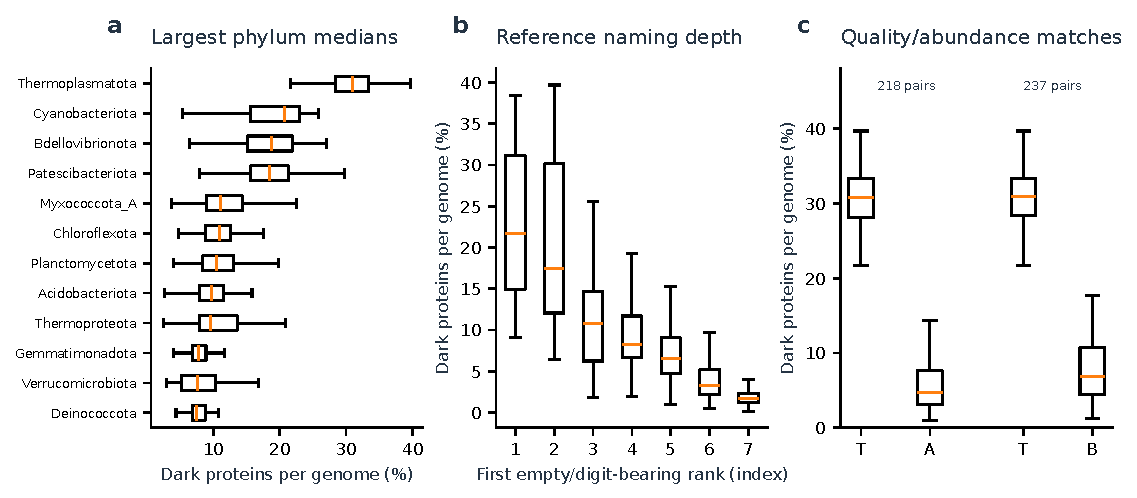
\includegraphics[width=\textwidth]{figures/fig_lineage_current.pdf}
\caption{\textbf{Lineage distribution, taxonomic naming depth and covariate-matched comparisons of assembly-cluster dark fractions.} \textbf{a}, The twelve highest median dark fractions among phyla with at least 20 representatives in the assembly-cluster contig tally (\texttt{v2\_reps.tsv.gz}; overall medians 31.0\% in Thermoplasmatota, 4.6\% in other archaea and 6.2\% in bacteria; compare reconciled representative Pyrodigal gene calls in main Fig.~\ref{fig:credibility}a with medians 30.4\%, 4.0\% and 5.4\%). \textbf{b}, Dark fraction by the first empty or digit-bearing label: 1, phylum; 2, class; 3, order; 4, family; 5, genus; 6, species; 7, no flagged rank. \textbf{c}, Thermoplasmatota (T) and matched other archaea (A) or bacteria (B), matched on completeness, contamination, corrected genome size, N50, abundance and prevalence (218 archaeal and 237 bacterial pairs). Boxes show the median and interquartile range; whiskers extend to 1.5 interquartile ranges.}
\label{fig:lineage}
\end{figure}

\begin{figure}[p]\centering
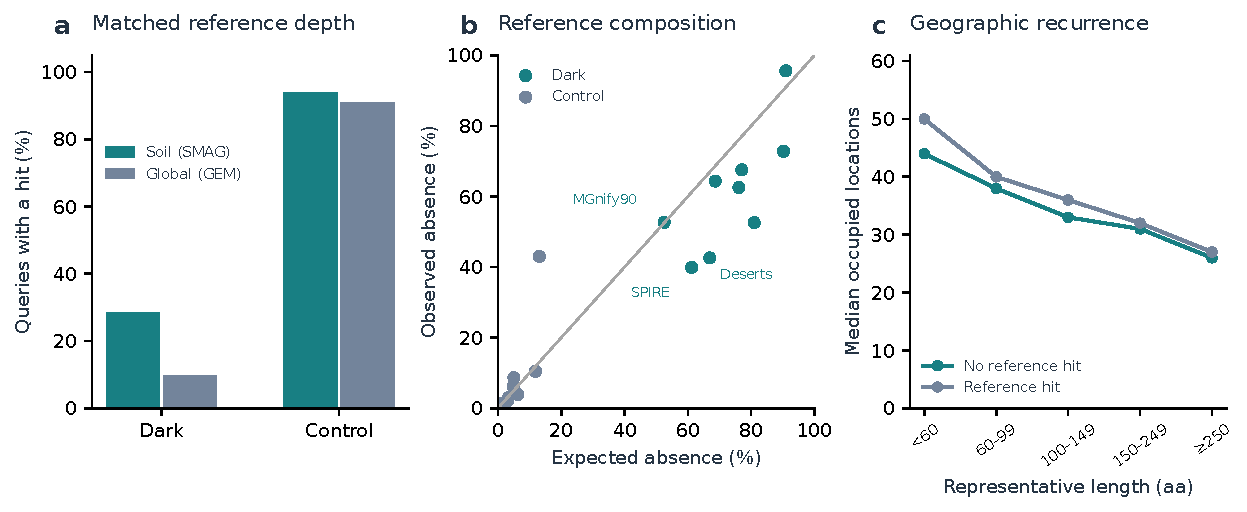
\includegraphics[width=\textwidth]{figures/fig_reference_atlas.pdf}
\caption{\textbf{External soil references recover recurrent desert families.} \textbf{a}, Hit rates for 106,042 dark and 106,042 UniRef50-matched queries against the primary SMAG and GEM panels. Protein counts and integer length distributions are identical between the two references. \textbf{b}, Observed absence versus analytical MGnify90 rarefaction expectations at the reference-catalogue sizes. Points below the diagonal have greater recovery than the size-only expectation. \textbf{c}, Median occupancy among 61 locations, stratified by representative length and absence from all searched catalogues.}
\label{fig:reference}
\end{figure}

\begin{figure}[p]\centering
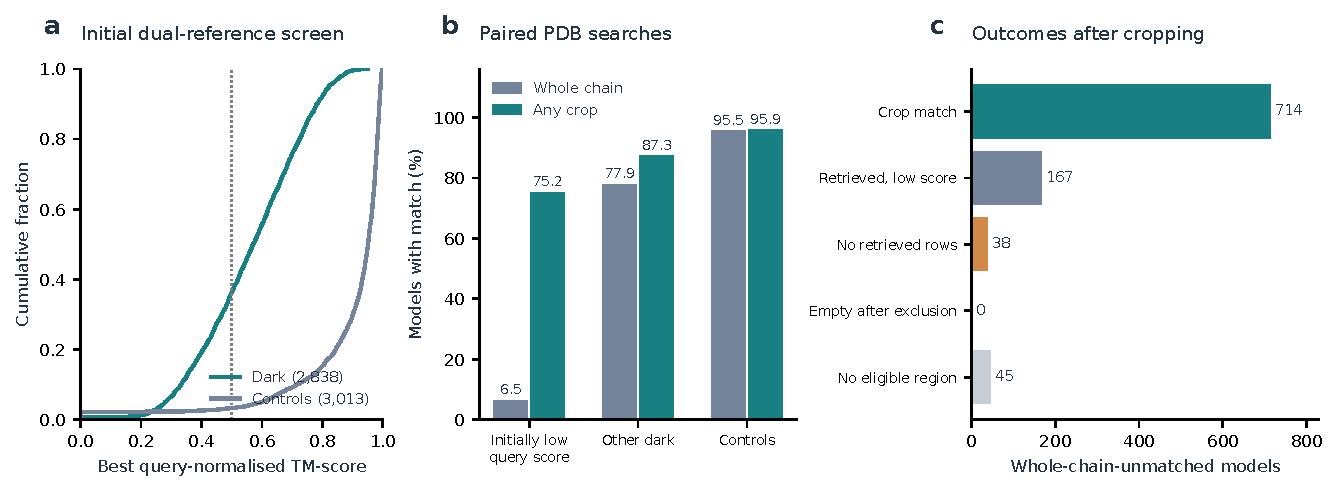
\includegraphics[width=\textwidth]{figures/fig_structure_current.pdf}
\caption{\textbf{Whole-chain and confident-region structural comparisons in the preliminary 2,838-model cohort.}
\textbf{a}, Best query-normalised TM-score across the initial PDB and AlphaFold references for 2{,}838 qualified dark models (from the preliminary 17,221-family screen) and 3{,}013 controls. The dashed line marks 0.5; zero retrievals are retained at zero. \textbf{b}, Whole-chain and any-crop match fractions in the paired CPU PDB search, with source entries excluded for controls (1{,}031 initial low-query-score dark models and 1{,}807 other dark models). \textbf{c}, Paired outcomes among the 964 same-run whole-chain-unmatched models in the initial low-query-score dark group; confident-region crops recover matches for 714 (74.07\%).}
\label{fig:structural}
\end{figure}

\begin{figure}[p]\centering
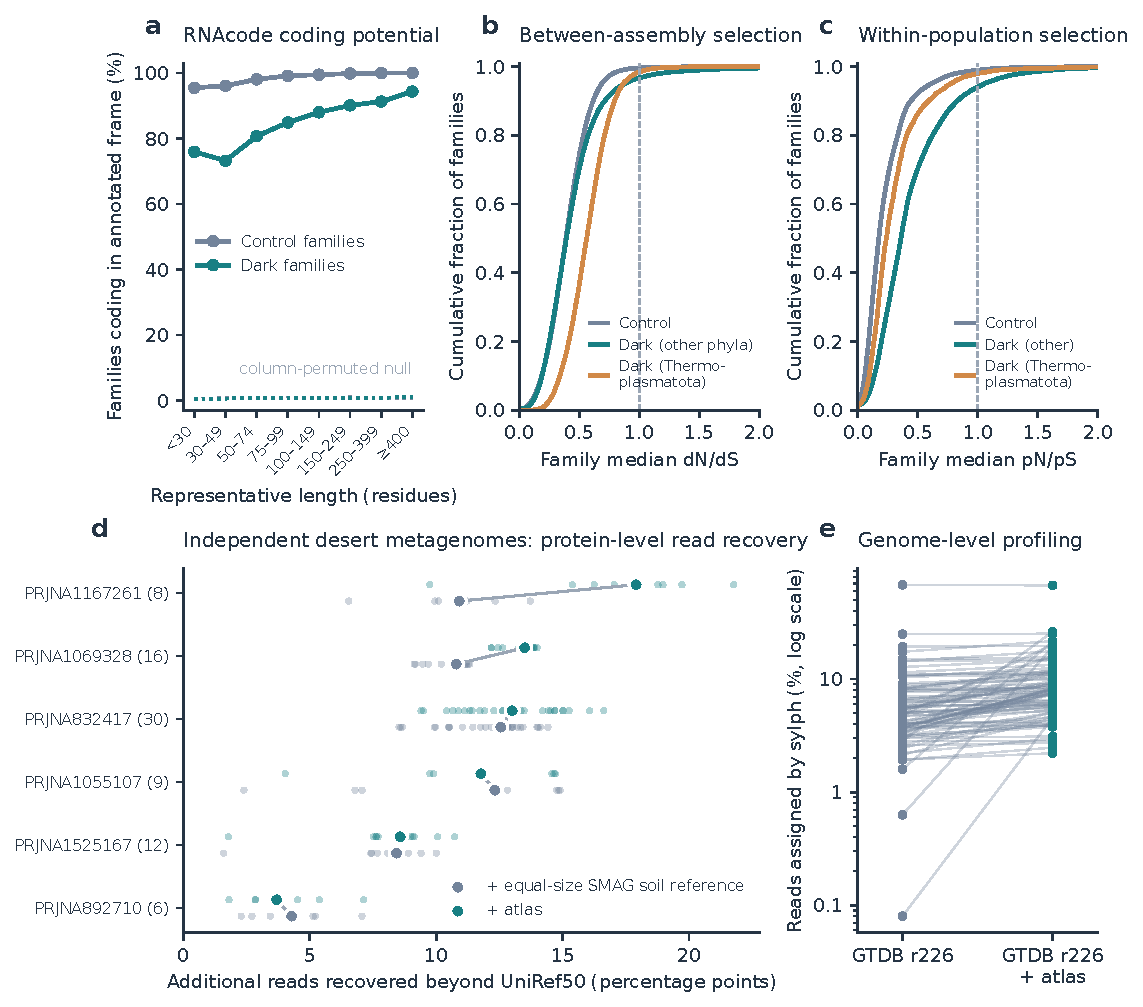
\includegraphics[width=\textwidth]{figures/fig_validation.pdf}
\caption{\textbf{Coding signatures and independent desert metagenome recovery benchmarks.}
\textbf{a}, Families with significant RNAcode coding potential in the annotated frame ($p<0.05$), by representative length, for 99,050 dark and 101,784 control families with at least three distinct members (also shown in main Fig.~\ref{fig:credibility}b).
\textbf{b}, Cumulative distributions of family median pairwise $\mathrm{dN/dS}$ (also shown in main Fig.~\ref{fig:credibility}c).
\textbf{c}, Cumulative distributions of family median $\mathrm{pN/pS}$ from read-level variant profiles in 551 metagenomes (also shown in main Fig.~\ref{fig:credibility}d).
\textbf{d}, Additional reads recovered beyond UniRef50 in translated searches of one million reads per run, after adding the 43.4-million genome-linked catalogue or an equal number of SMAG soil cluster representatives, for 81 runs from six independent desert soil studies.
\textbf{e}, Reads assigned by sylph against GTDB r226 with and without the 5,438 desert species representatives.}
\label{fig:validation}
\end{figure}
